\newcommand{\SFWTAGHPWPT} {$1.03 \pm 0.03~\rm{(stat)} \pm 0.04~\rm{(sys)} \pm 0.06~\rm{(sys)}$}
\newcommand{\SFWTAGLPWPT} {$0.88 \pm 0.12~\rm{(stat)} \pm 0.17~\rm{(sys)} \pm 0.12~\rm{(sys)}$}
\newcommand{\SFWTAGHPWPL} {\ensuremath{1.01\pm0.03}\xspace}
\newcommand{\SFWTAGLPWPL} {\ensuremath{0.78\pm0.87}\xspace}
\newcommand{\UNCWTAGHPWPT} {\ensuremath{13\%}\xspace} 
\newcommand{\UNCWTAGLPWPT} {\ensuremath{56\%}\xspace}
\newcommand{\UNCWTAGHPWPL} {\ensuremath{10\%}\xspace}
\newcommand{\UNCWTAGLPWPL} {\ensuremath{26\%}\xspace}
\newcommand{\WMASSDATAWPT}{\ensuremath{81.9\pm0.3}\xspace}
\newcommand{\WRESDATAWPT} {\ensuremath{8.9\pm0.4}\xspace}
\newcommand{\WMASSMCWPT}  {\ensuremath{82.0\pm0.2}\xspace}
\newcommand{\WRESMCWPT}   {\ensuremath{8.3\pm0.3}\xspace}
\newcommand{\JMS}         {$0.999 \pm 0.004~\rm{(stat)} \pm 0.0006~\rm{(sys)}$}
\newcommand{\JMR}         {$1.08 \pm 0.07~\rm{(stat)} \pm 0.08~\rm{(sys)}$}
\section{Towards robust boosted jet tagging}
\label{sec:searchII:intro}
When we first studied W tagging with 13 \TeV data, in the context of the analysis conducted with the 2015 dataset, Section~\ref{sec:searchI:wtagging}, two interesting correlations were observed:
\bigskip
\begin{enumerate}[1)]
\item a strong dependence of the jet mass on the jet \PT, when using the AK8 jet clustering algorithm with CHS pileup removal and softdrop with $\beta = 0$ (mMDT) grooming, and
\item a strong dependence of the \nsubj selection efficiency on pileup, when using the AK8 jet clustering algorithm with CHS pileup removal.
\end{enumerate}
\bigskip
\noindent The reason we studied the softdrop algorithm with $\beta = 0$, hereafter just referred to as "softdrop", as an alternative to the pruning algorithm used in the 2015 analysis was that, besides the possibility that it might perform better, we knew it had certain favorable qualities compared to other groomers; the softdrop algorithm, in addition to removing sensitivity to the soft divergences of QCD as all groomers do (they are IRC safe, see Section~\ref{sec:objreco:irc}), eliminates all correlated soft emissions in the jet which are wider than the dominant two-prong substructure, leading to no non-global logarithmic terms (NGLs) in the jet mass~\cite{Dasgupta:2013ihk}. NGLs arise from configurations where, for instance, a soft gluon is radiated into the jet cone, as illustrated in Figure~\ref{fig:searchII:ngls}. 
\begin{figure}[h!]
\centering
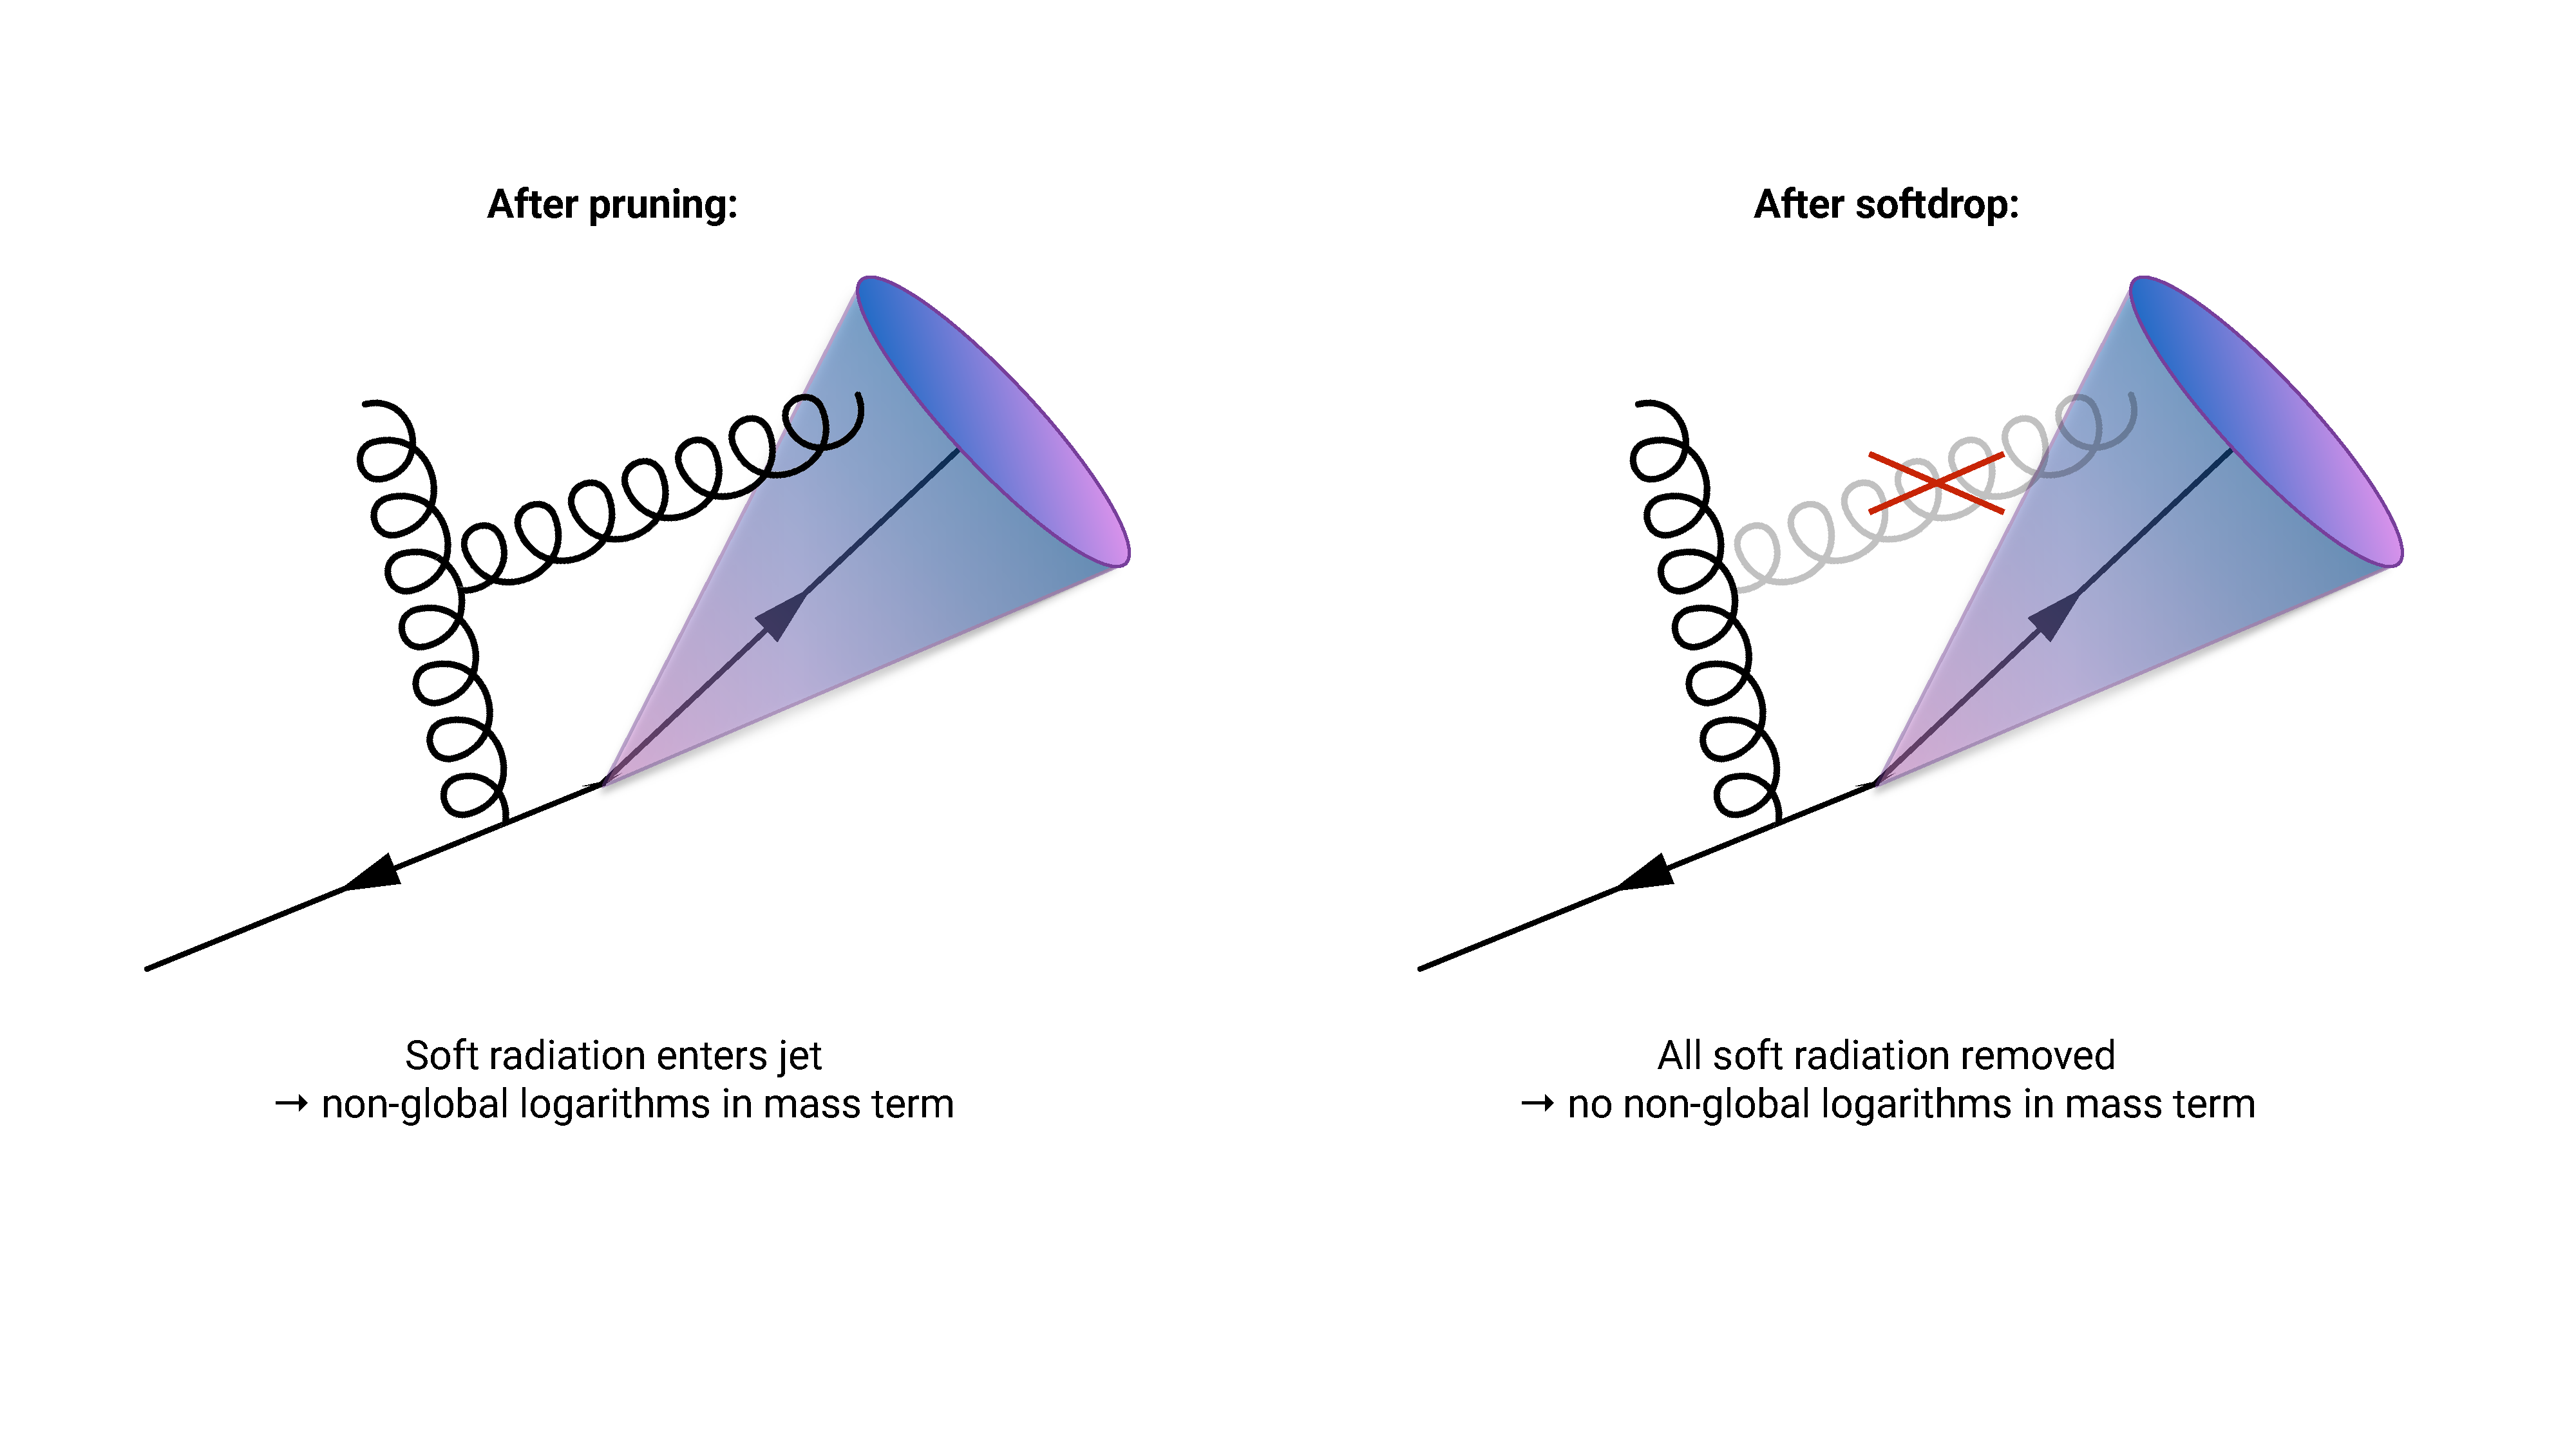
\includegraphics[width=0.69\textwidth]{figures/analysis/search2/misc/ngls.pdf}
\caption{The pruning algorithm does not remove all soft emission and therefore has non-global logarithmic terms in the jet mass. Softdrop with $\beta = 0$ removes all soft emissions wider than the dominant two-prong substructure and is therefore free of non-global logarithms.}
\label{fig:searchII:ngls}
\end{figure}
The benefit of being NGL-free, is that one can calculate the softdrop jet mass to a significantly higher precision than what is possible for other grooming algorithms or for the plain jet mass (NGLs are the main reason a full resummation of the plain jet mass beyond NLL accuracy does not exist). There were therefore theoretically well-motivated reasons for wanting the baseline CMS vector boson tagger to be softdrop-based.\par 
However, as was discussed in Section~\ref{sec:searchI:wtagging}, the softdrop jet-mass of signal jets displayed a large dependence on jet \PT, both for reconstructed and generator-level jets. One hypothesis was that this was due to pileup and that perhaps softdrop was more sensitive to contribution from additional interaction vertices than pruning. A study in Ref.~\cite{Dasgupta:2015yua} had also shown mMDT to be more sensitive to the underlying event, but using a different asymmetry criteria than softdrop (see Appendix~\ref{app:sdue}).\par
In parallel to the ongoing theoretical work on groomers, a novel pileup removal algorithm had been proposed: Pileup per particle identification (PUPPI)~\cite{Bertolini2014}. Described in detail in Section~\ref{subsub:objreco:puppi}, PUPPI considers not only charged pileup, but also reweights neutral particles in the jet with its probability of arising from pileup. PUPPI had proven itself far superior to the current CHS algorithm in terms of jet observables for large radius jets, and therefore seemed like a good candidate to address both issues listed above: the softdrop \PT dependence and the strong pileup dependence of $\tau_{21}$. The focus of Search II would therefore be on the commissioning of a novel W-tagger. There are interesting additions to the analysis strategy as well: the inclusion of a $\PZpr \rightarrow \WW$ signal hypothesis and the addition of a completely new analysis, the single V-tag analysis.

\section{Analysis strategy}
The analysis strategy for this search is conceptually the same as for Search I. In addition, we take advantage of the n-subjettiness categorization and do an additional analysis in parallel: a search for excited quark resonances $\rm{q^*}$~\cite{Bauer1987,PhysRevD.42.815} decaying to qW or qZ.
We call this the single V-tag analysis, and the analysis selection only differs in that one jet is not required to pass the V-tag selection (groomed mass and n-subjettiness). The \VV analysis is hereby referred to as the double V-tag analysis. The difference between the two analyses is illustrated in Figure~\ref{fig:searchII:svsd}. 
\begin{figure}[h!]
\centering
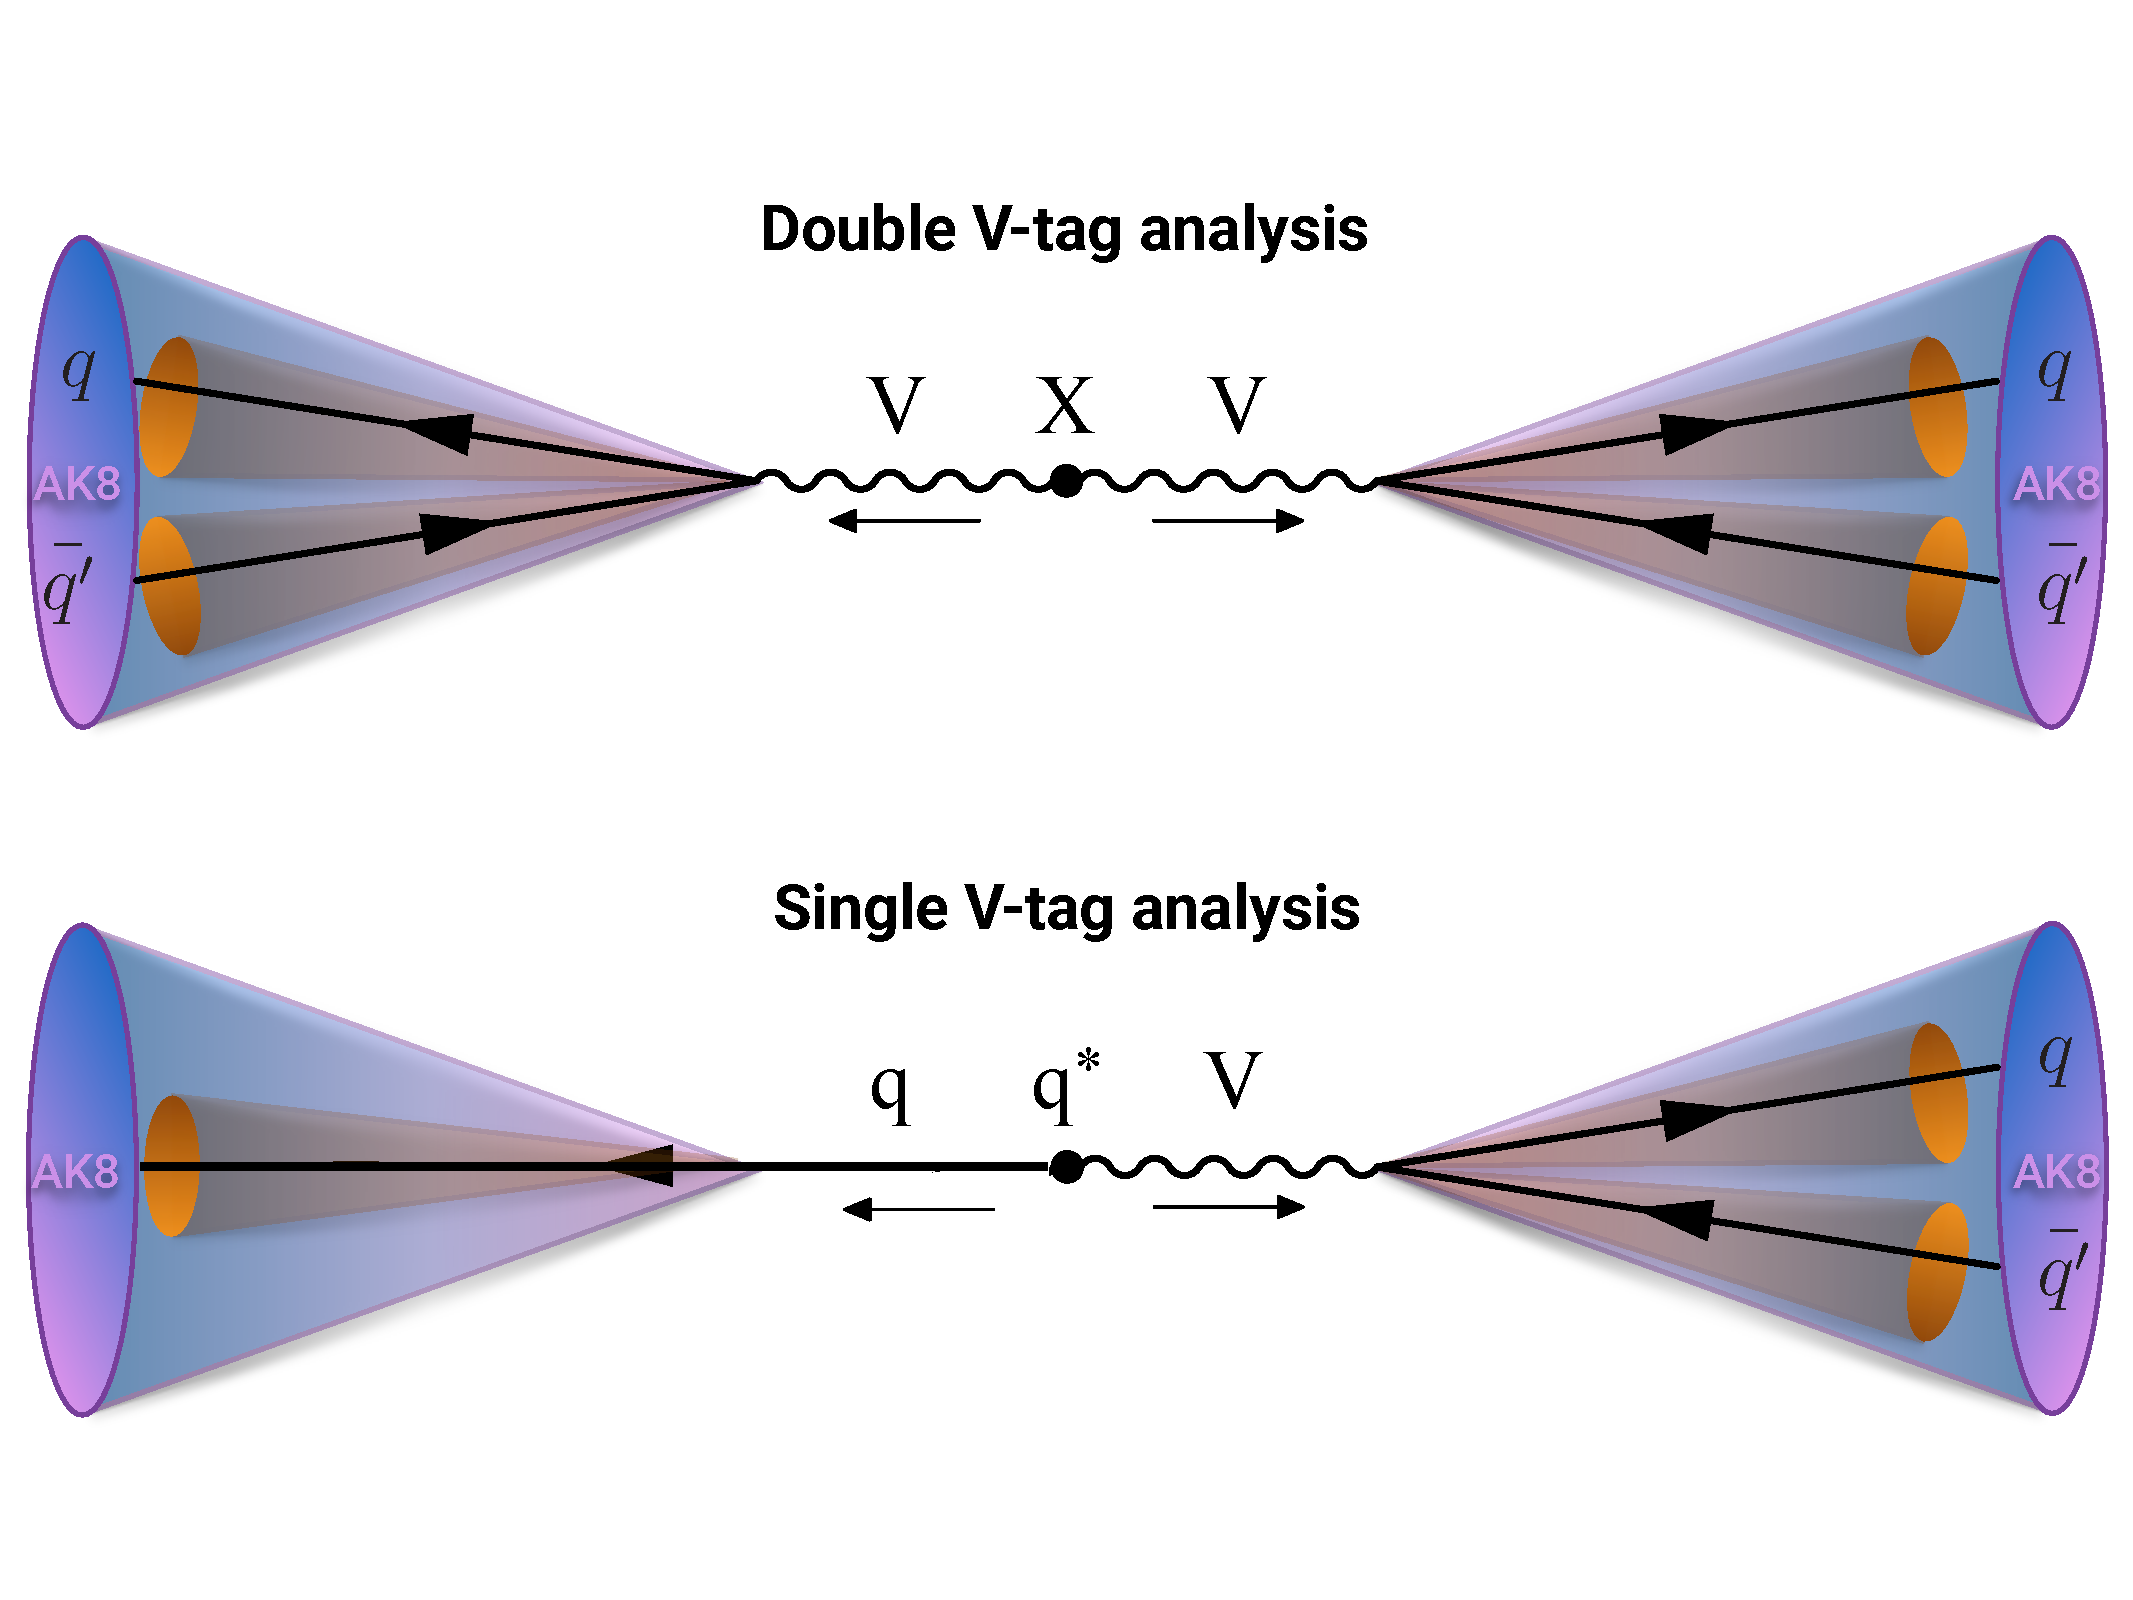
\includegraphics[height=6.5cm]{figures/analysis/search2/misc/singlevsdoubletag.pdf}
\caption{The double (top) and single (bottom) W/Z-tag analysis.}
\label{fig:searchII:svsd}
\end{figure}
In addition, limits are set on a $\PZpr \rightarrow \WW$ signal hypothesis in the double V-tag analysis, another first with data collected at 13 TeV center-of-mass energy.
This analysis was published in two steps: an early CMS physics analysis summary document (PAS) based on 12.9 \fbinv of 2016 data~\cite{CMS-PAS-B2G-16-021}, describing the new PUPPI softdrop based V tagger as well as the single V-tag analysis, and a second analysis considering the full 2016 dataset~\cite{PhysRevD.97.072006}. The commissioning of the new V tagger has also been documented in a jet performance PAS~\cite{CMS-PAS-JME-16-003}. In this chapter, the main emphasis will be on the work presented in CMS-PAS-B2G-16-021~\cite{CMS-PAS-B2G-16-021} since this was were the new V tagger and single V-tag analysis was first presented. The second part of the results chapter, Section~\ref{sec:searchII:brg17001res}, includes the results obtained using the full 2016 dataset of 35.9 \fbinv.

\section{Data and simulated samples}
\label{sec:searchII:samples}
As mentioned above, the analysis of the 2016 dataset was done in two steps corresponding to two different datasets: one analysis based on 12.9 \fbinv of early 2016 data, describing the new W-tagger and single V-tag category, and a second paper considering the full 2016 dataset, corresponding to 35.9 \fbinv. Both were collected at a center-of-mass energy of 13 TeV.\par
The \BulkG and HVT signal samples are modeled in the same way as in 2015. The $\textrm{q}^*$ samples are simulated assuming unpolarized bosons and a compositeness scale $\Lambda$ set equal to the resonance mass. These are generated at leading order using \PYTHIA version 8.212~\cite{Sjostrand:2007gs}. \par
The standard model background processes of QCD, W+jets, and Z+jets are all simulated to leading order. The W and Z+jets backgrounds are simulated with \amcatnlo~\cite{Alwall:2014hca,Alwall:2007fs}. Three different combinations of matrix element and shower generators are used for QCD as these predictions are known to differ: \PYTHIA-only, the leading order mode of \amcatnlo{} matched with \PYTHIA, and \HERWIG{++}~2.7.1~\cite{Bahr:2008pv} with the CUETHS1 tune~\cite{Khachatryan:2015pea}.

\section{Event selection}
\subsection{Triggering}
The triggers used in this analysis are the same ones as in 2015 (see Section~\ref{sec:searchI:trigger}), however, due to the new single V-tag analysis, the trigger turn-ons have been reevaluated separately with the requirement that either one or two jets have an offline softdrop jet mass above 65 \GeV. Figure~\ref{fig:searchII:trigger-fits} shows the trigger turn-on curves as a function of dijet invariant mass for jets passing one of the \HT-based triggers only (pink markers), one of the grooming triggers only (green markers), and when combining all of them (purple markers). The turn-on curves are shown for all jet pairs passing loose selections as described in Section \ref{sec:searchI:preselection} (top), and for jet pairs where one (bottom left) or both (bottom right) of the jets additionally are required to have a softdrop mass larger than 65 GeV.
\begin{figure}[h!]
\centering
% 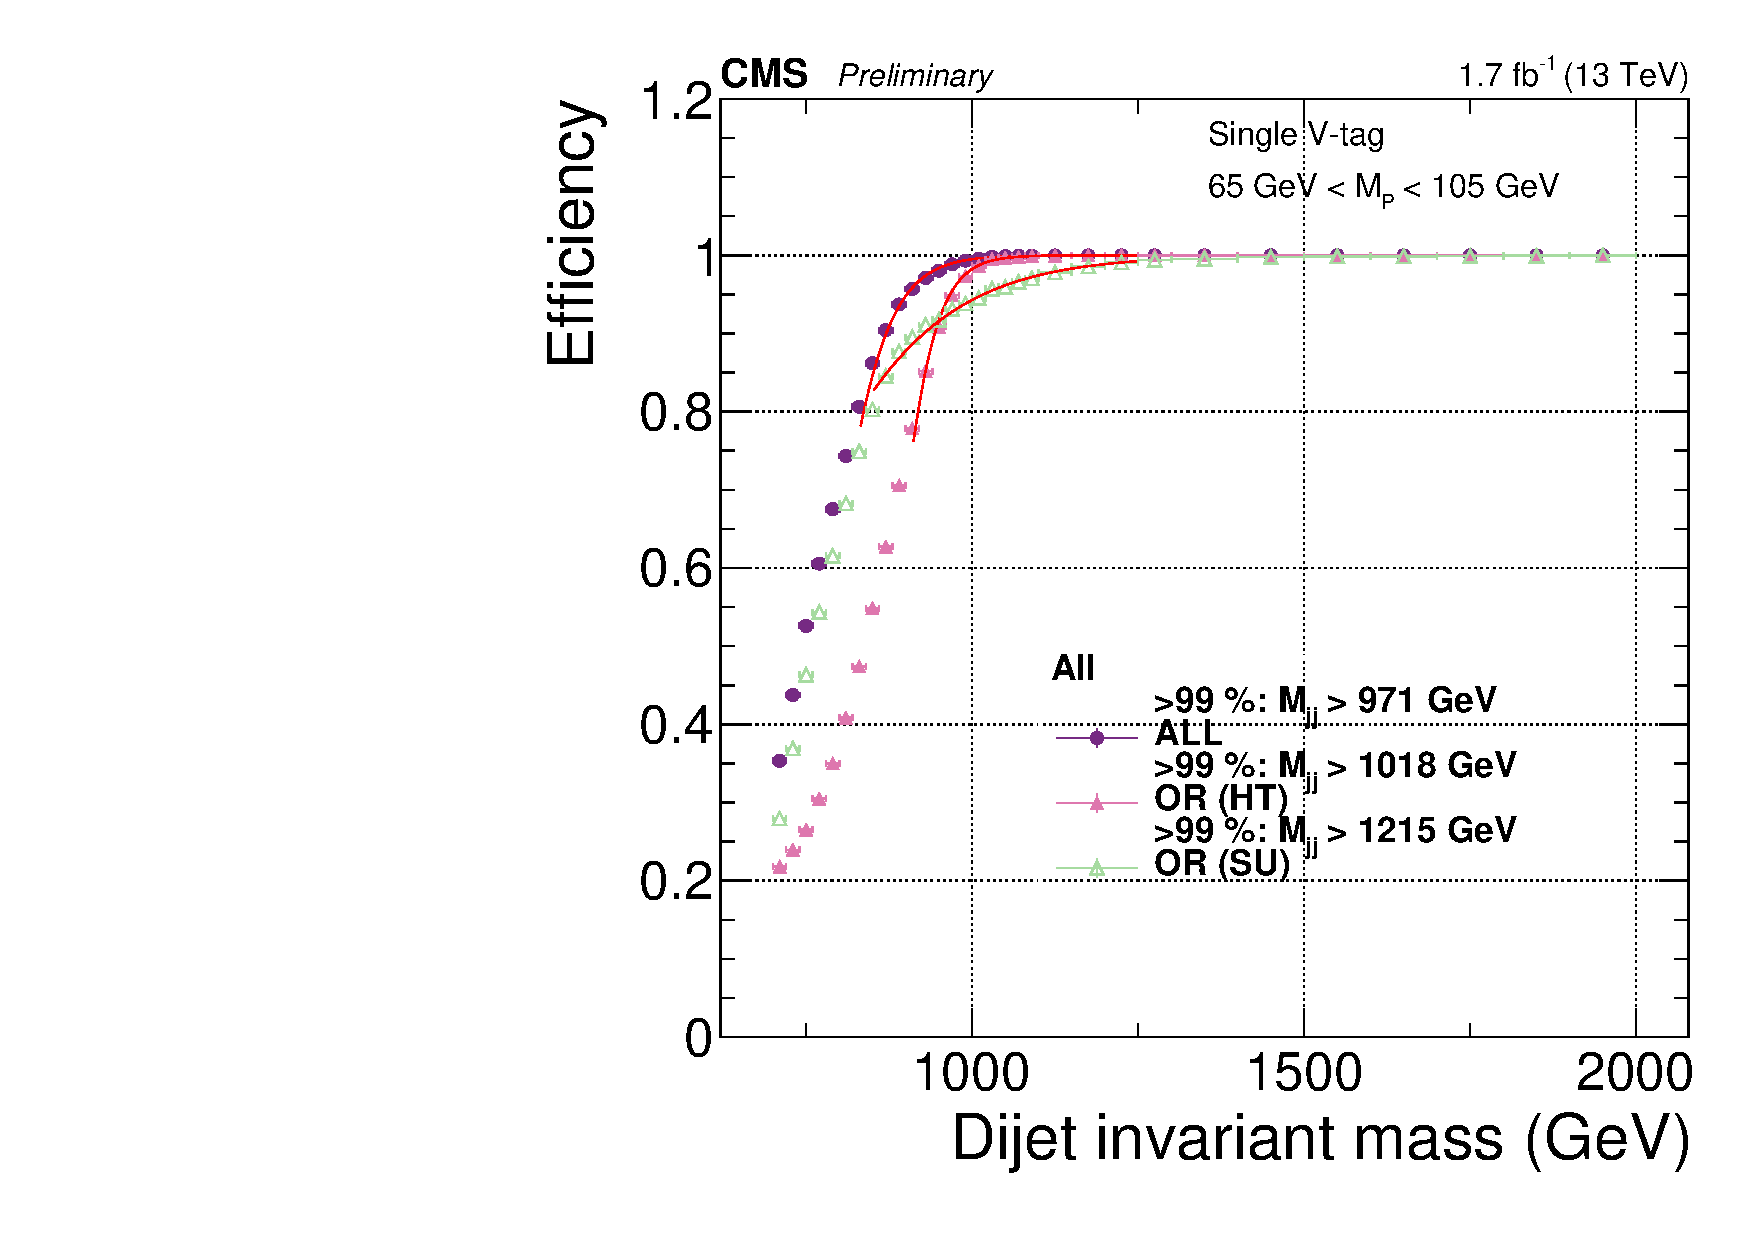
\includegraphics[width=0.4\textwidth]{figures/analysis/search2/AN-16-398/plots/trigger/triggereffMjj-ALL_SingleTag_runAll.pdf}
% 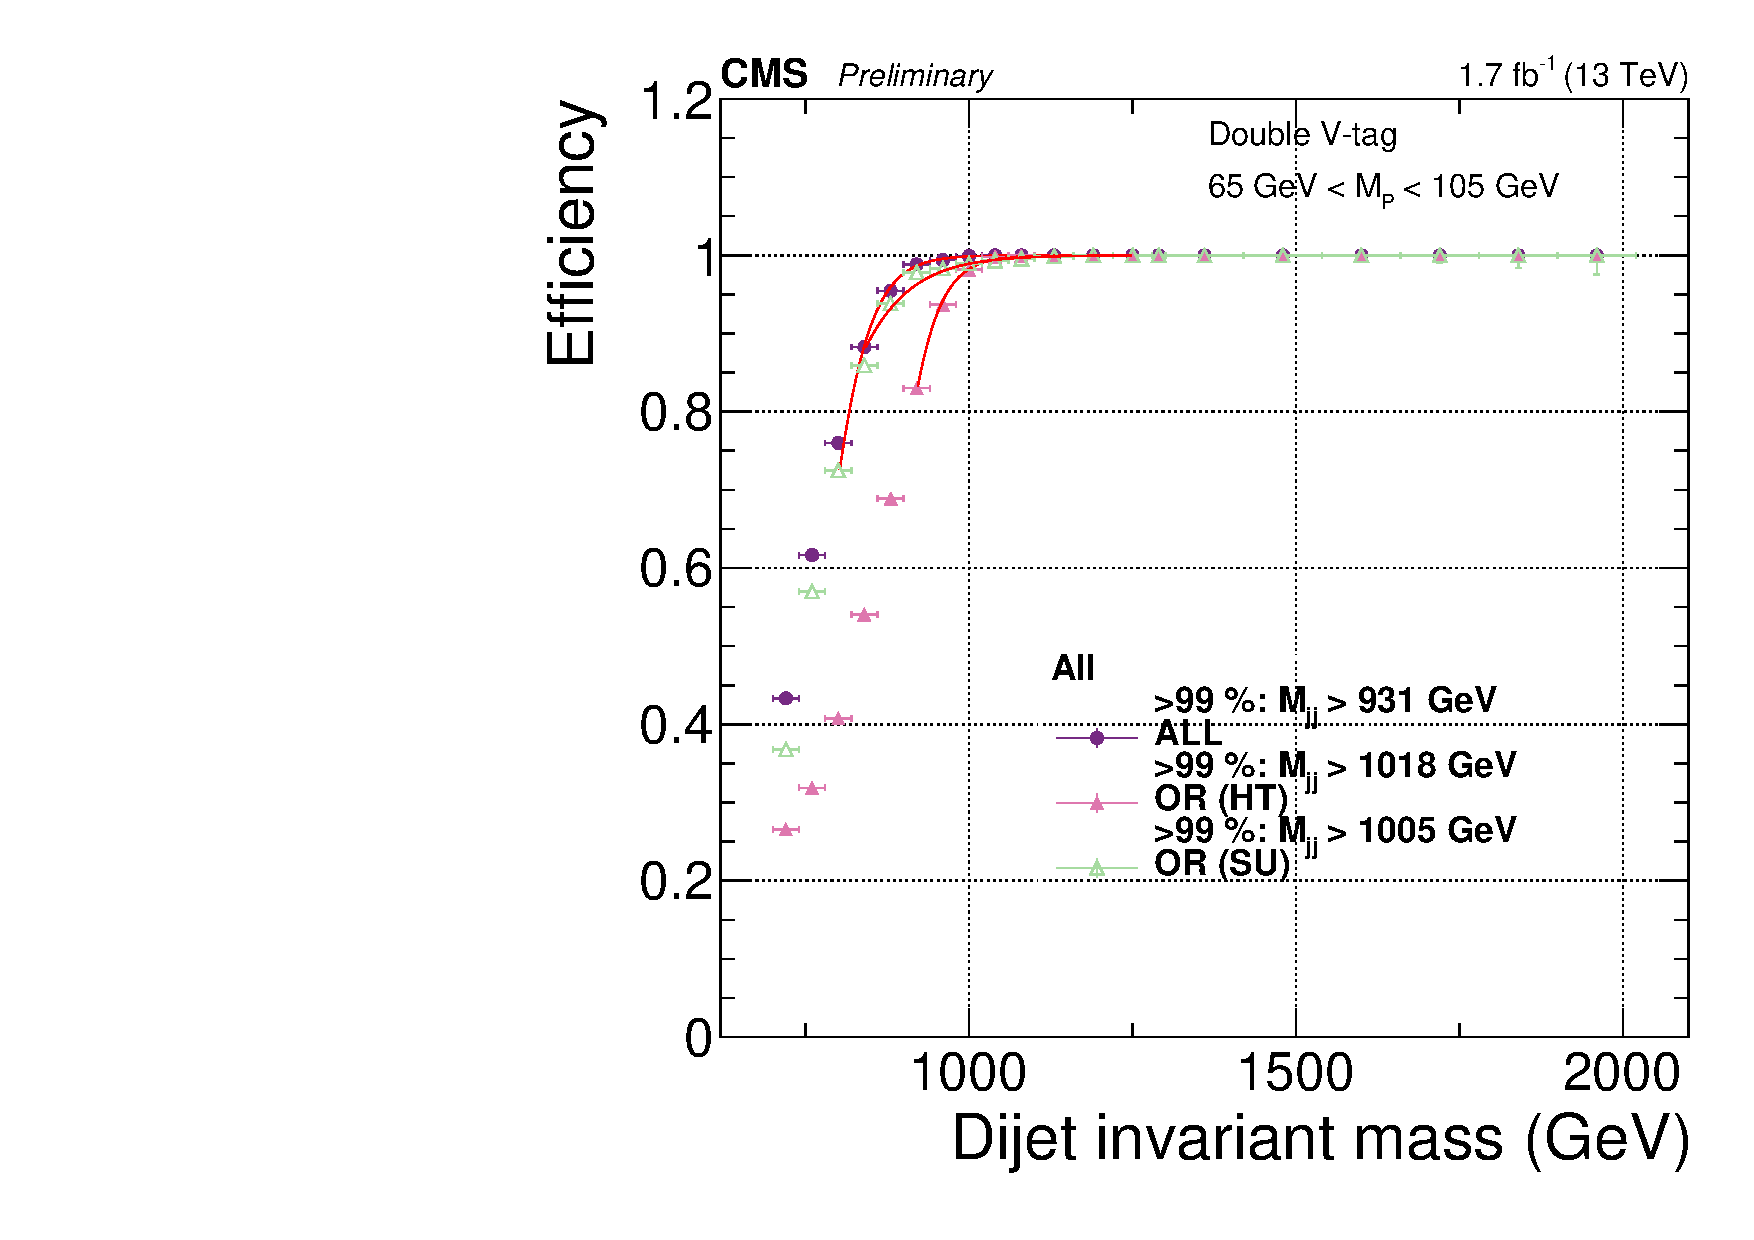
\includegraphics[width=0.4\textwidth]{figures/analysis/search2/AN-16-398/plots/trigger/triggereffMjj-ALL_DoubleTag_runAll.pdf}
% 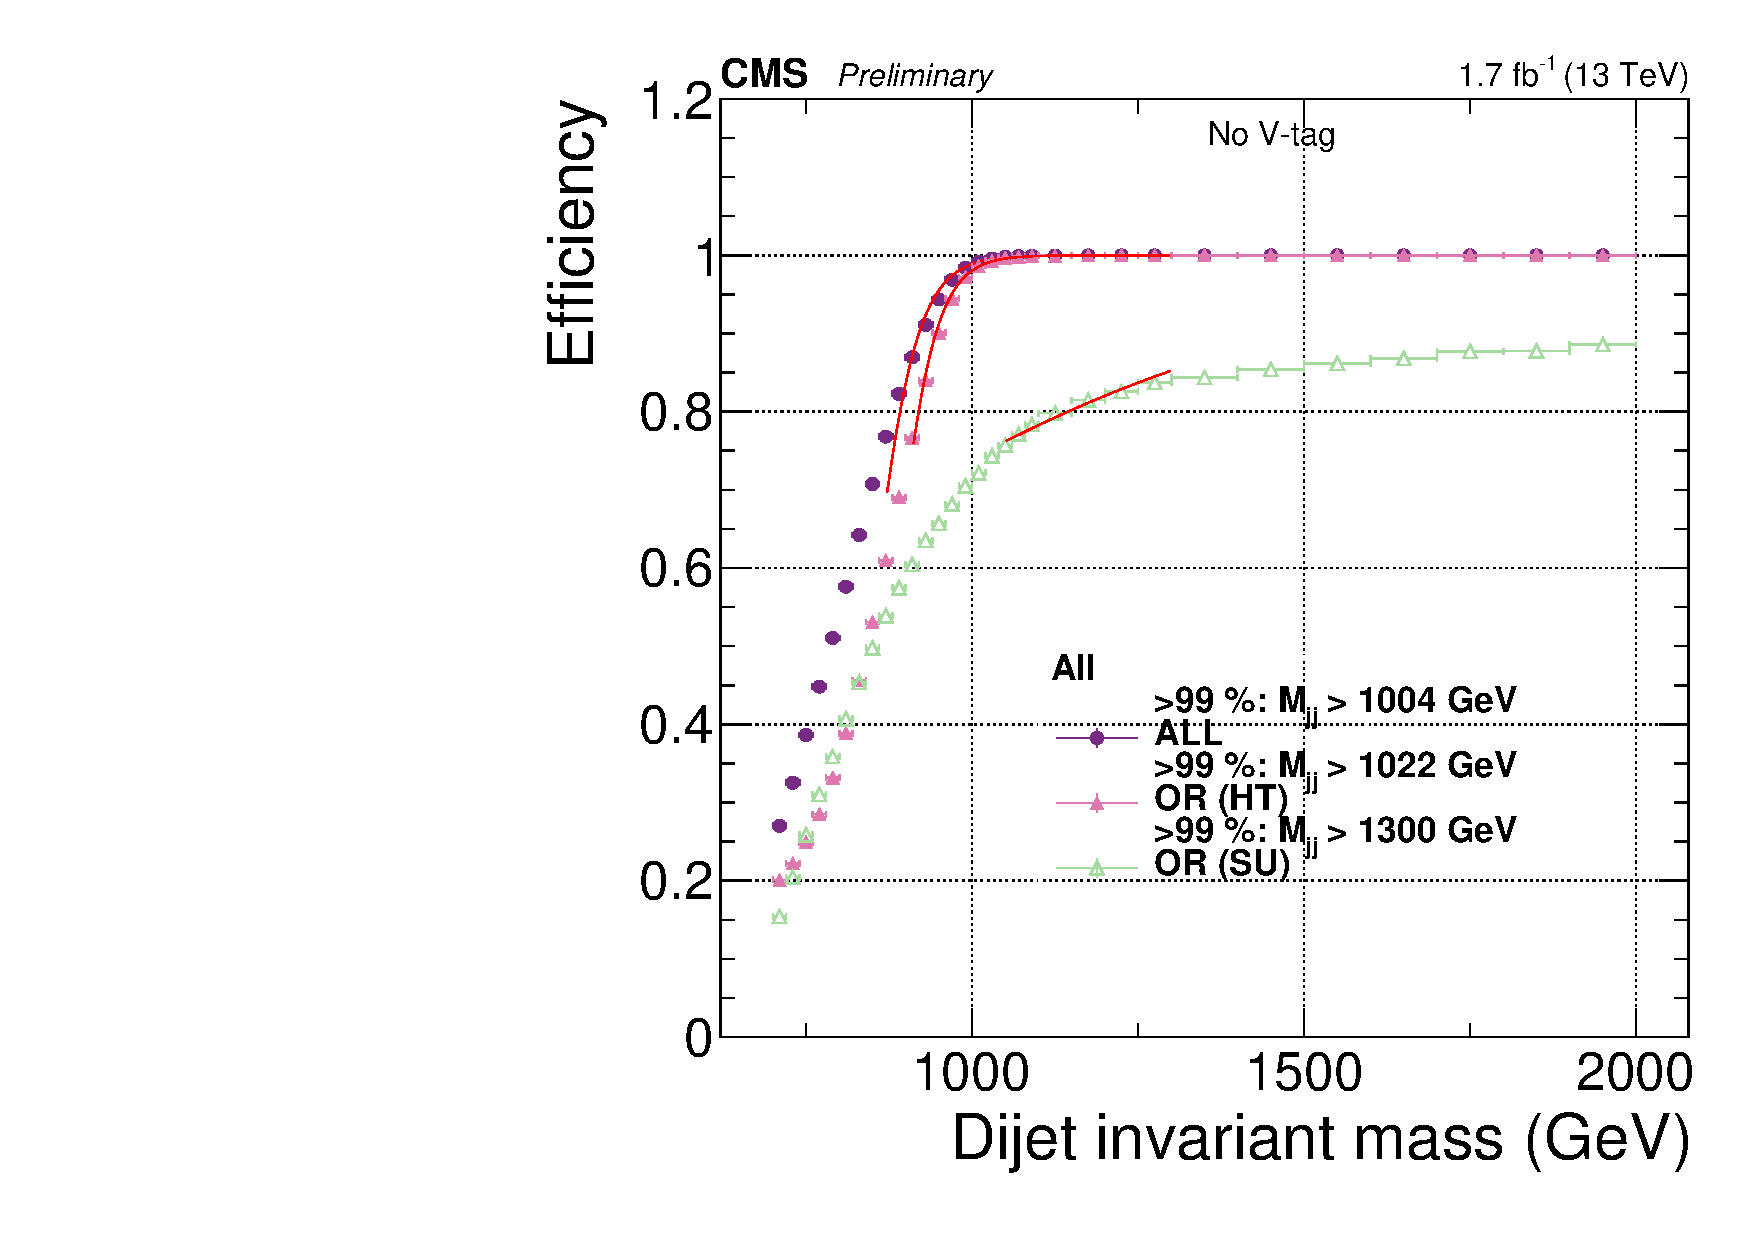
\includegraphics[width=0.4\textwidth]{figures/analysis/search2/AN-16-398/plots/trigger/triggereffMjj-ALL_noTag_runAll.pdf}
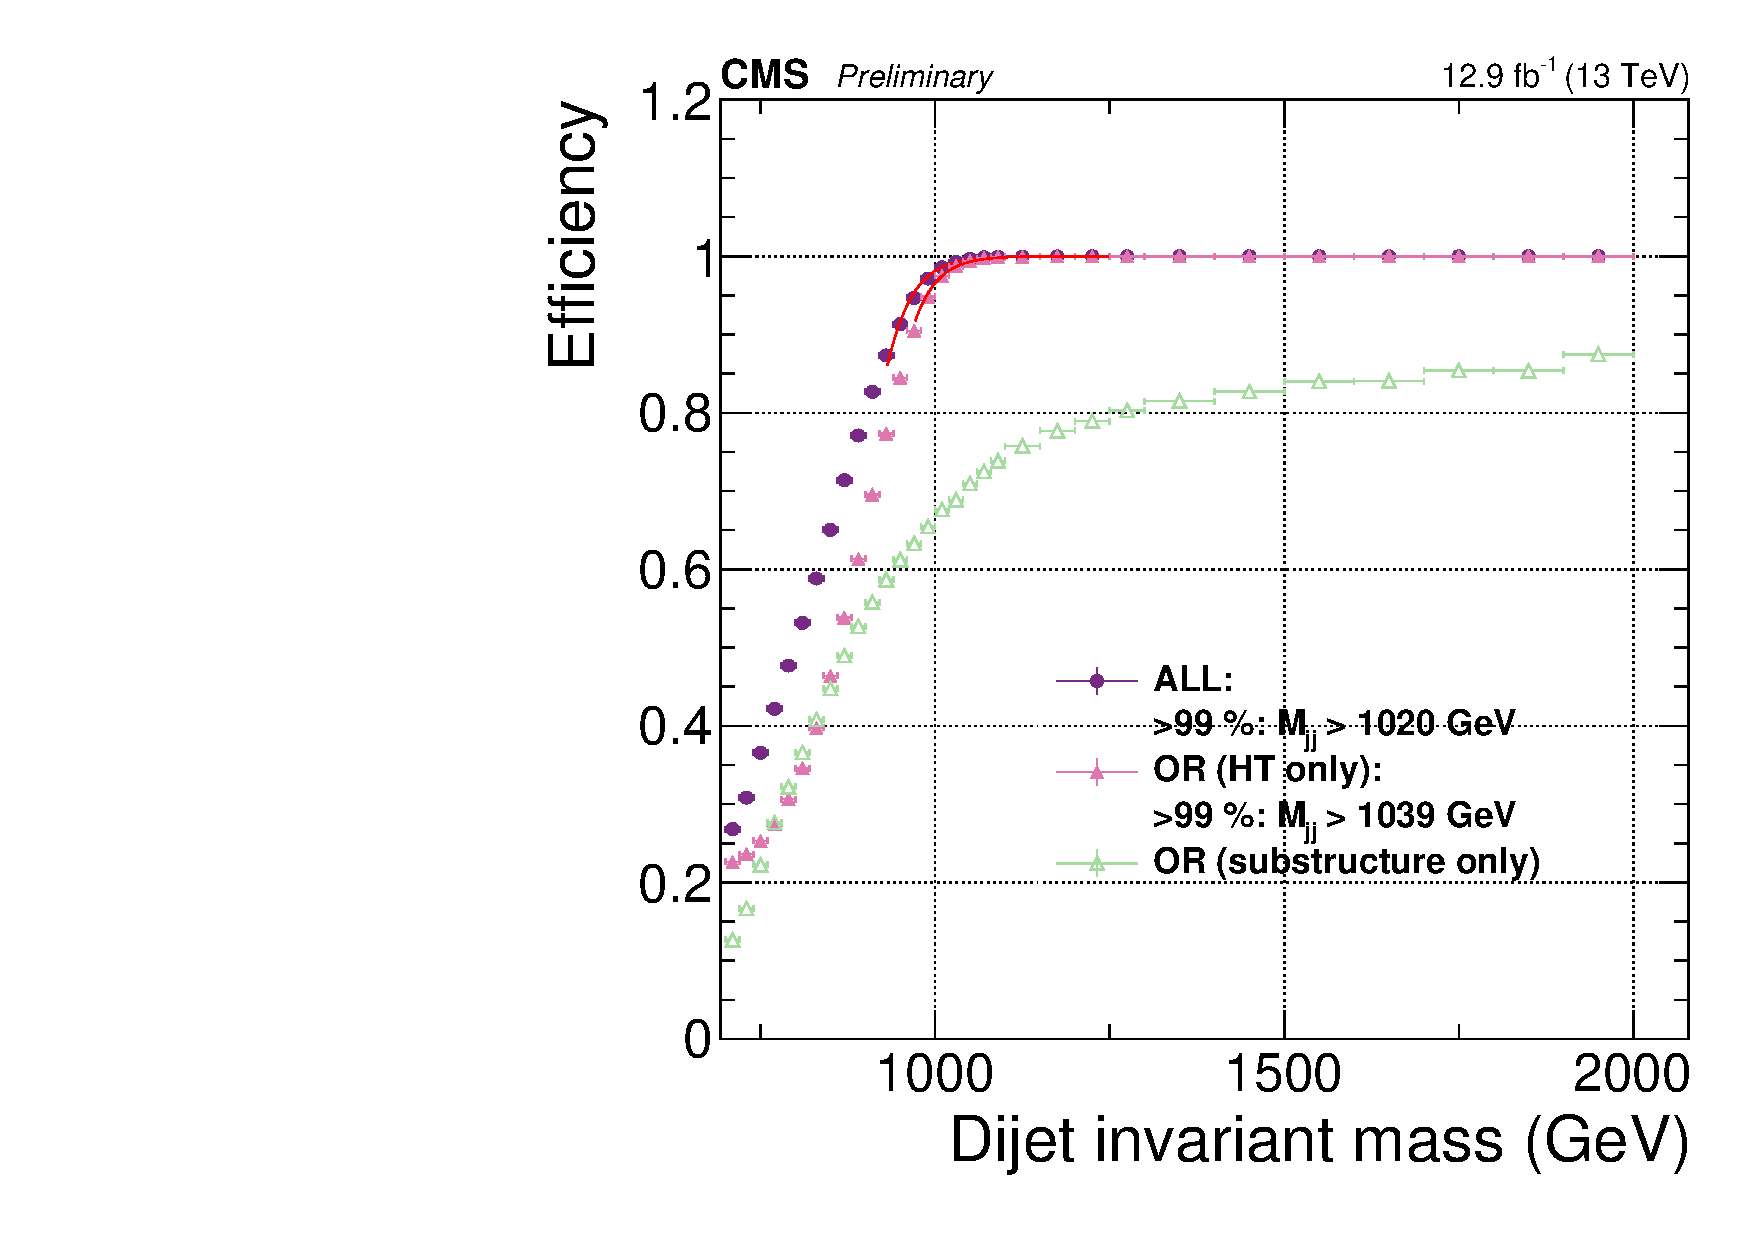
\includegraphics[width=0.49\textwidth]{figures/analysis/search2/AN-16-235/plots/triggereffMjj-ALL_noTag.pdf}
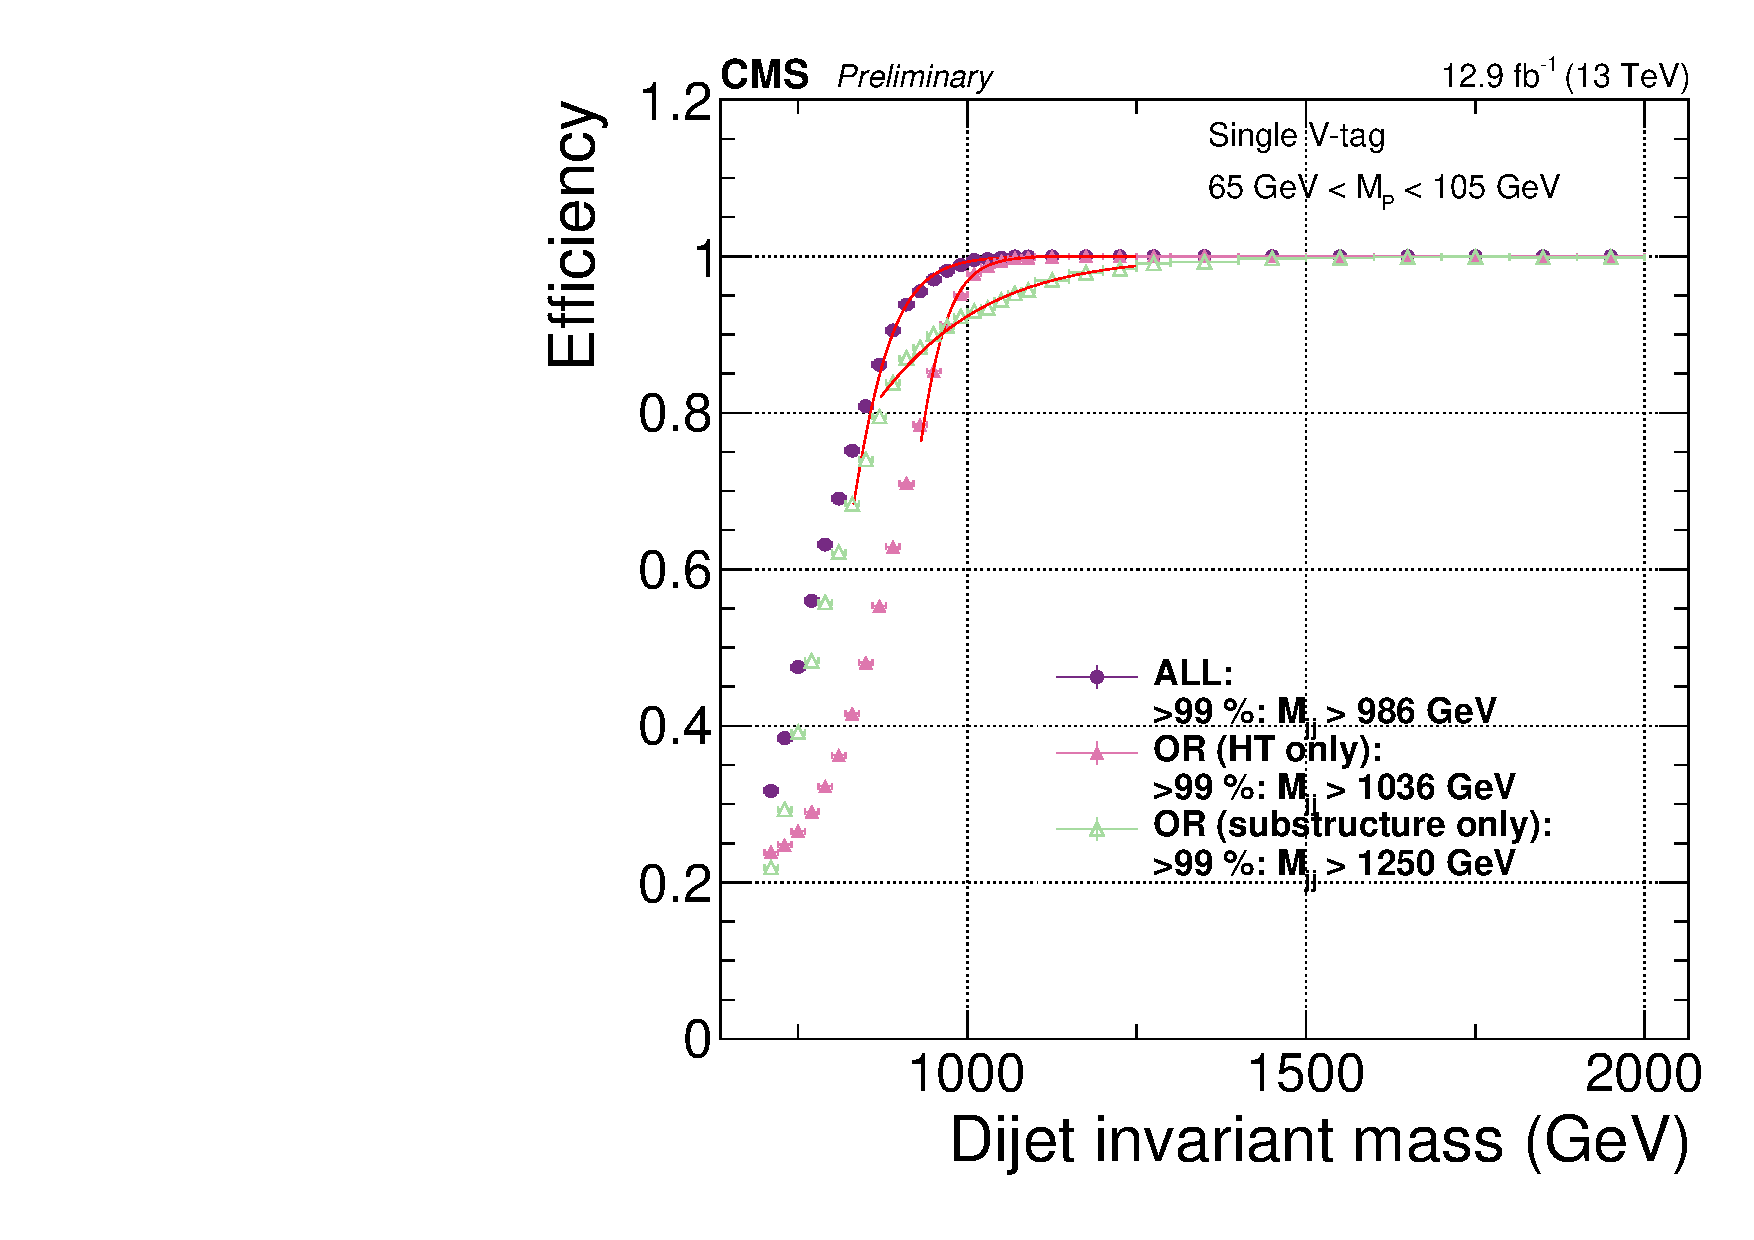
\includegraphics[width=0.49\textwidth]{figures/analysis/search2/AN-16-235/plots/triggereffMjj-ALL_SingleTag.pdf}
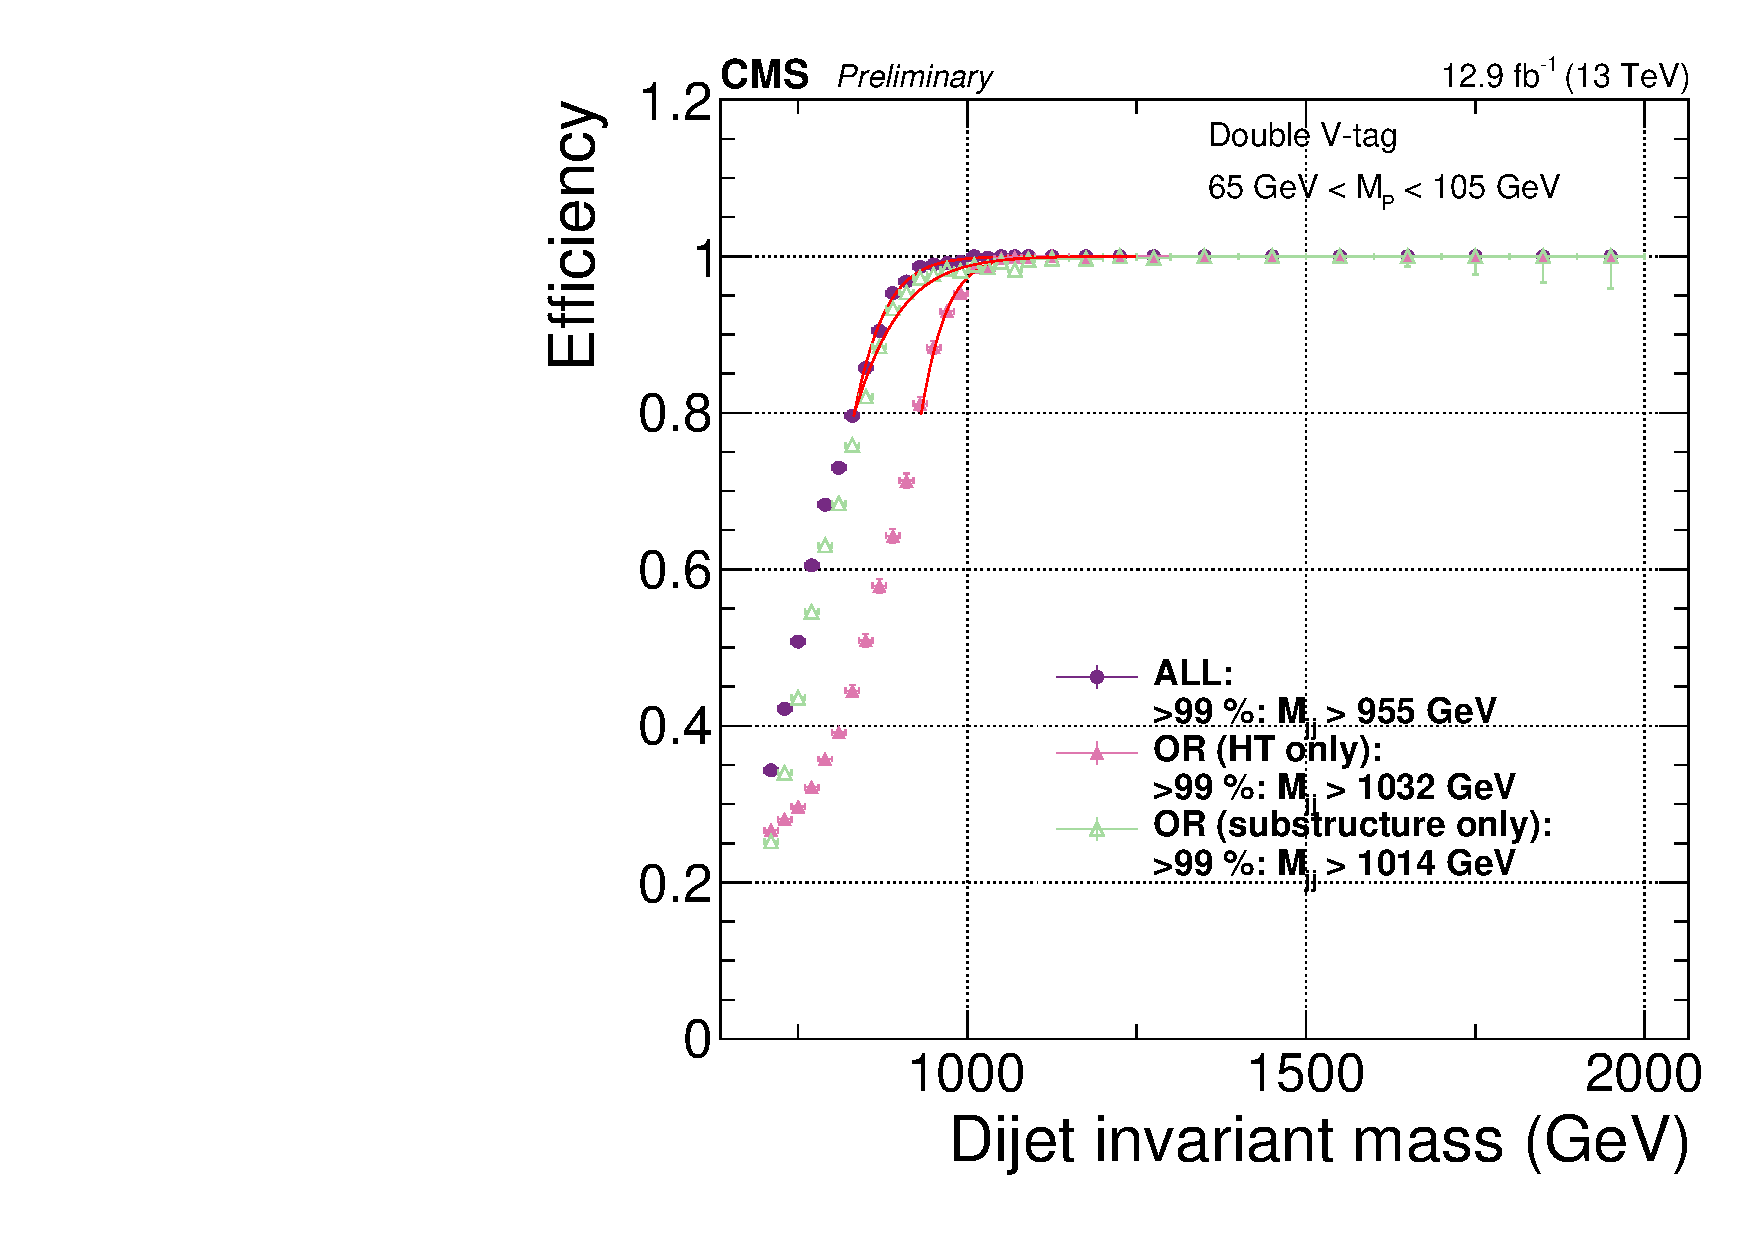
\includegraphics[width=0.49\textwidth]{figures/analysis/search2/AN-16-235/plots/triggereffMjj-ALL_DoubleTag.pdf}\\
\caption{Comparison of trigger efficiencies for jets passing one of the HT-triggers only (pink), for jets passing one of the grooming-triggers only (green), and for jets passing one of the HT-triggers or one of the grooming triggers (purple). It is shown here as a function of the dijet invariant mass for all jet pairs passing loose selections (top), where one jet additionally is required to have a softdrop mass larger than 65 GeV (bottom left), and where both jets are required to have a softdrop mass larger than 65 GeV (bottom right).}
\label{fig:searchII:trigger-fits}
\end{figure}
\noindent Including the grooming triggers lowers the 99\% trigger efficiency threshold by around 50 (80) \GeV in the single-tag (double-tag) category once substructure is required on the analysis level. Using a combination of either of the triggers, we are safely on the trigger plateau for dijet invariant masses above 955 (986) \GeV in the double (single) tag category, so that the dijet invariant-mass threshold can be set at 955 GeV for the double-tag analysis and 990 \GeV for the single-tag analysis. For control plots, where no groomed-mass window is applied, a trigger threshold of 1020 GeV is used. Figure~\ref{fig:searchII:grooming-mj-trigger} shows the trigger efficiency as a function of the offline PUPPI softdrop-jet mass (left) and pruned-jet mass (right) for the trigger requiring an online trimmed-jet mass of at least 30 \GeV. Here, the jet transverse momentum of one of the jets is required to be at least 600 GeV and no other mass cut is applied. The trigger turn-on is sharp and the plateau is reached for offline groomed-jet masses around 50 GeV.
\begin{figure}[h!]
\centering
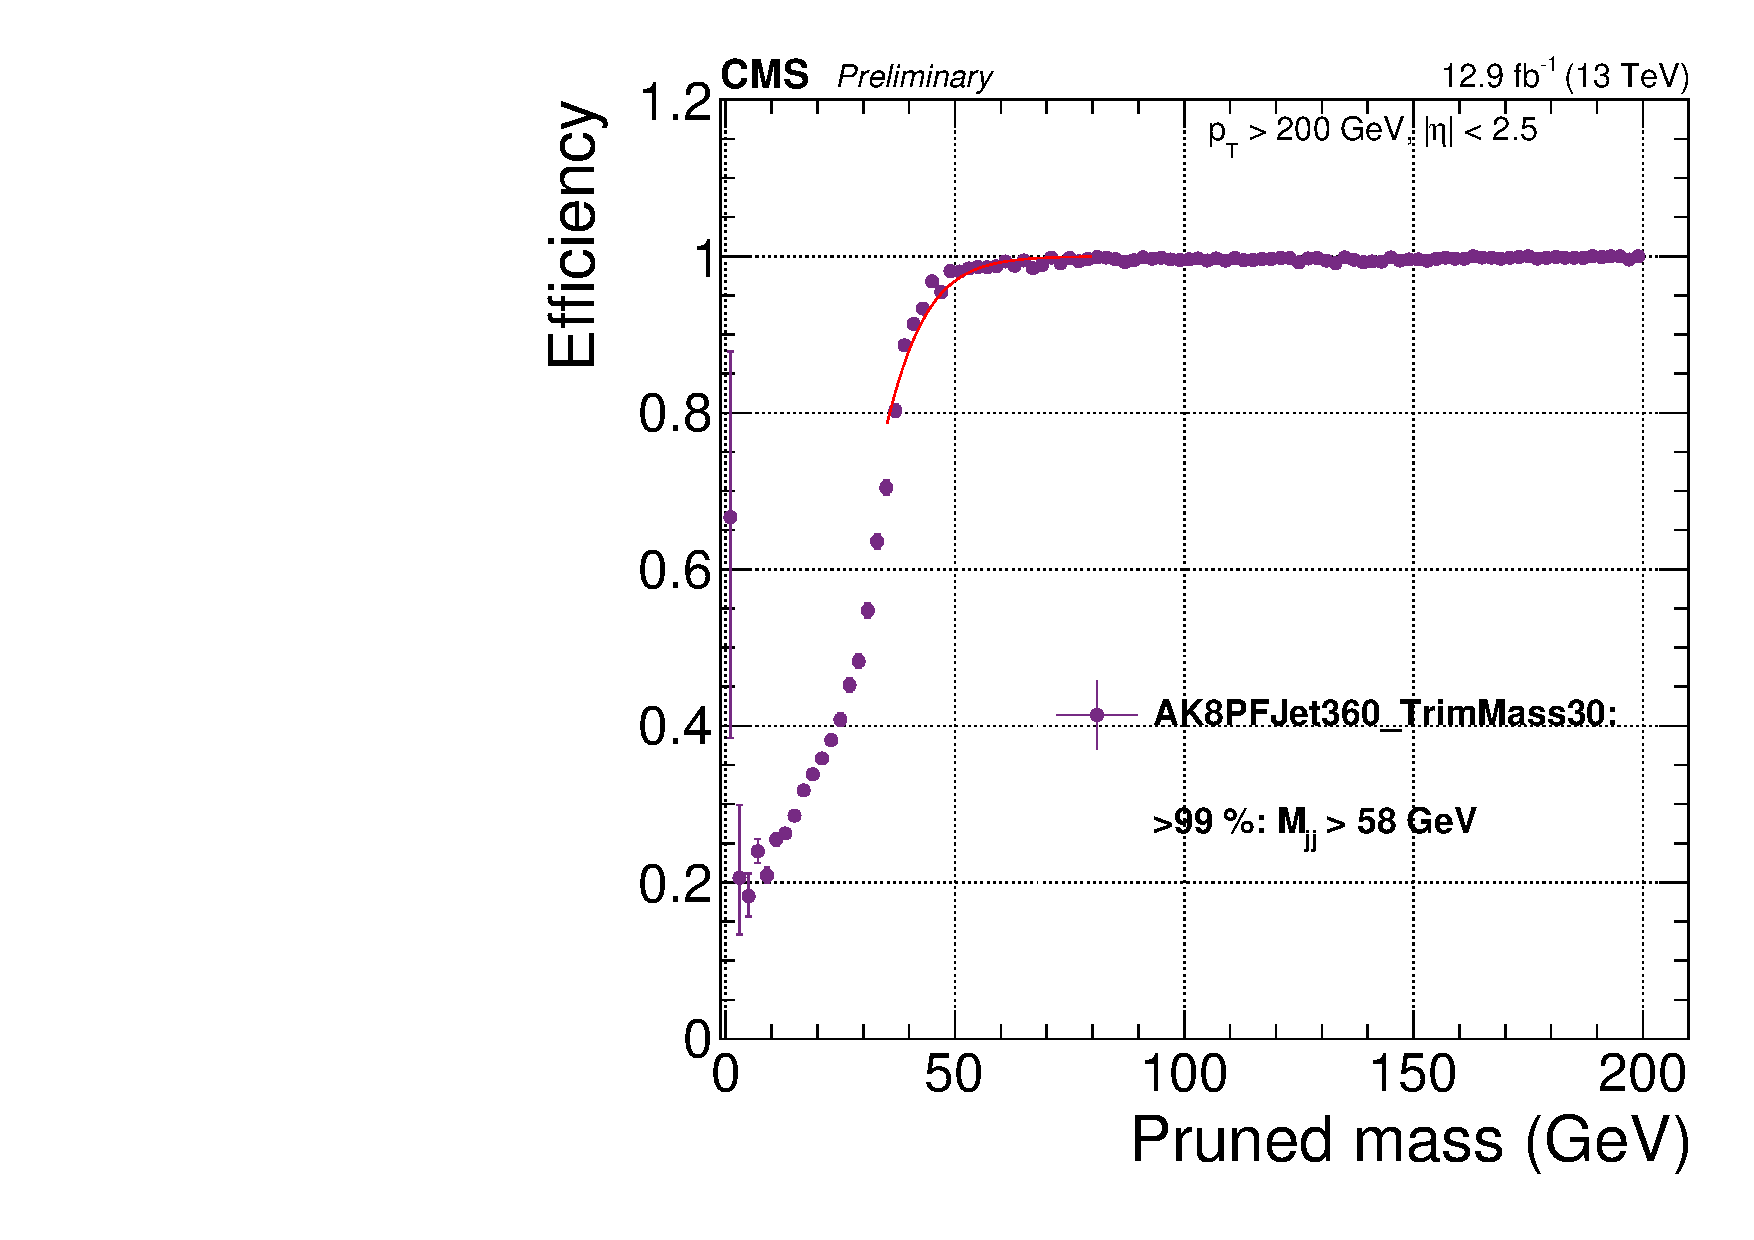
\includegraphics[width=0.49\textwidth]{figures/analysis/search2/AN-16-235/plots/triggereff-prunedmass_fit.pdf}
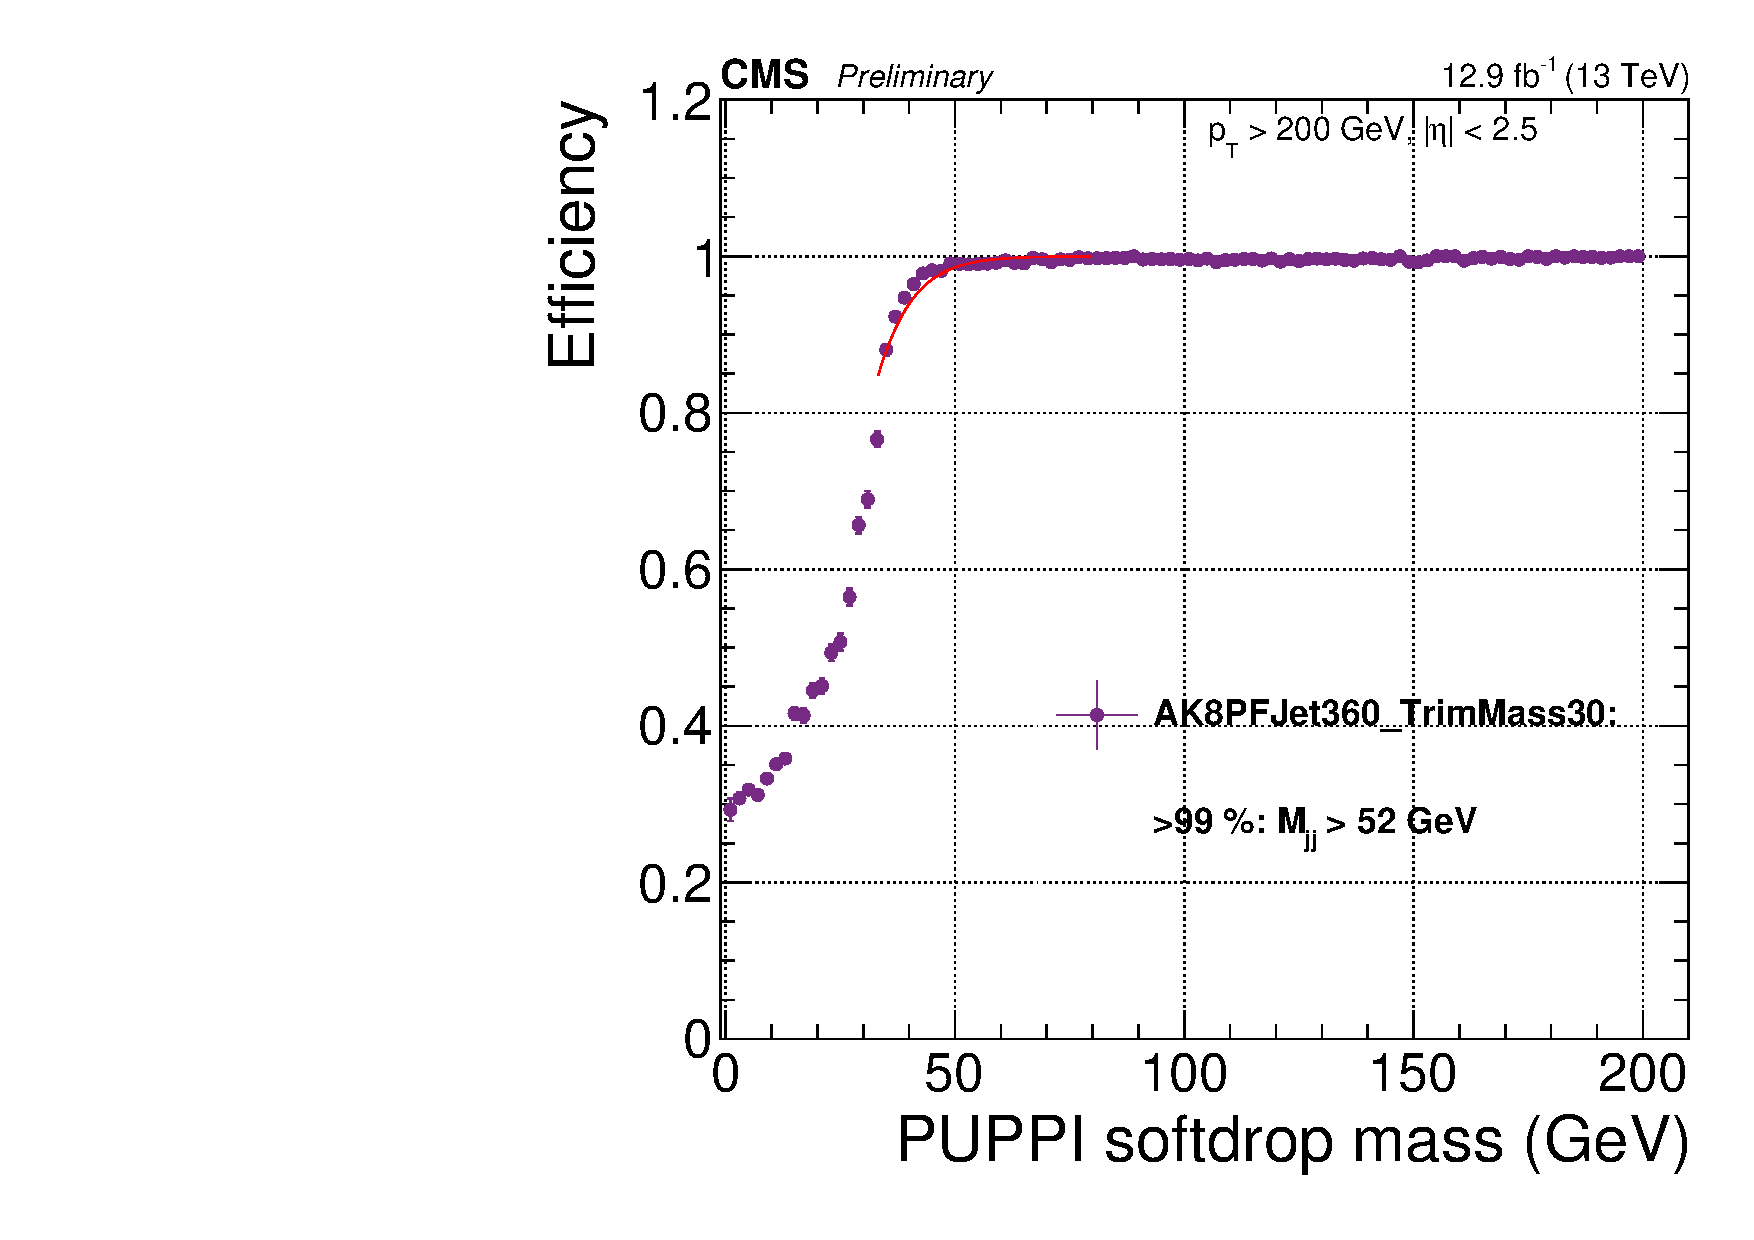
\includegraphics[width=0.49\textwidth]{figures/analysis/search2/AN-16-235/plots/triggereff-sdmass_fit.pdf}
\caption{Efficiency for the trigger requiring an online trimmed jet mass of at least 30 \GeV as a function of the pruned-jet (left) and softdrop-jet (right) mass for jets with $\PT > \unit{600}{\GeV}$.}
\label{fig:searchII:grooming-mj-trigger}
\end{figure}

\subsection{Preselection}
\label{sec:searchII:presel}
The same preselections as in Search I, described in Section~\ref{sec:searchI:preselection}, are used; we require two AK8 jets with CHS pileup subtraction applied, and that are required to pass the tight jet-ID requirement, $\PT>200 \GeV$ and $|\eta|<2.5$. The same selection requirement that suppresses t-channel QCD production is required, $|\Delta \eta|<1.3$, together with thresholds on the dijet invariant mass of 955 GeV for the double-tag and 990 GeV for the single-tag analyses. The jet \PT (top left), $\eta$ (top right), $\Delta \eta_{jj}$ (bottom left) and dijet invariant mass (bottom right) for the two leading jets in the event after loose preselections are applied is shown in Figure~\ref{fig:searchII:kinematics-all}.
\begin{figure}[h!]
\centering
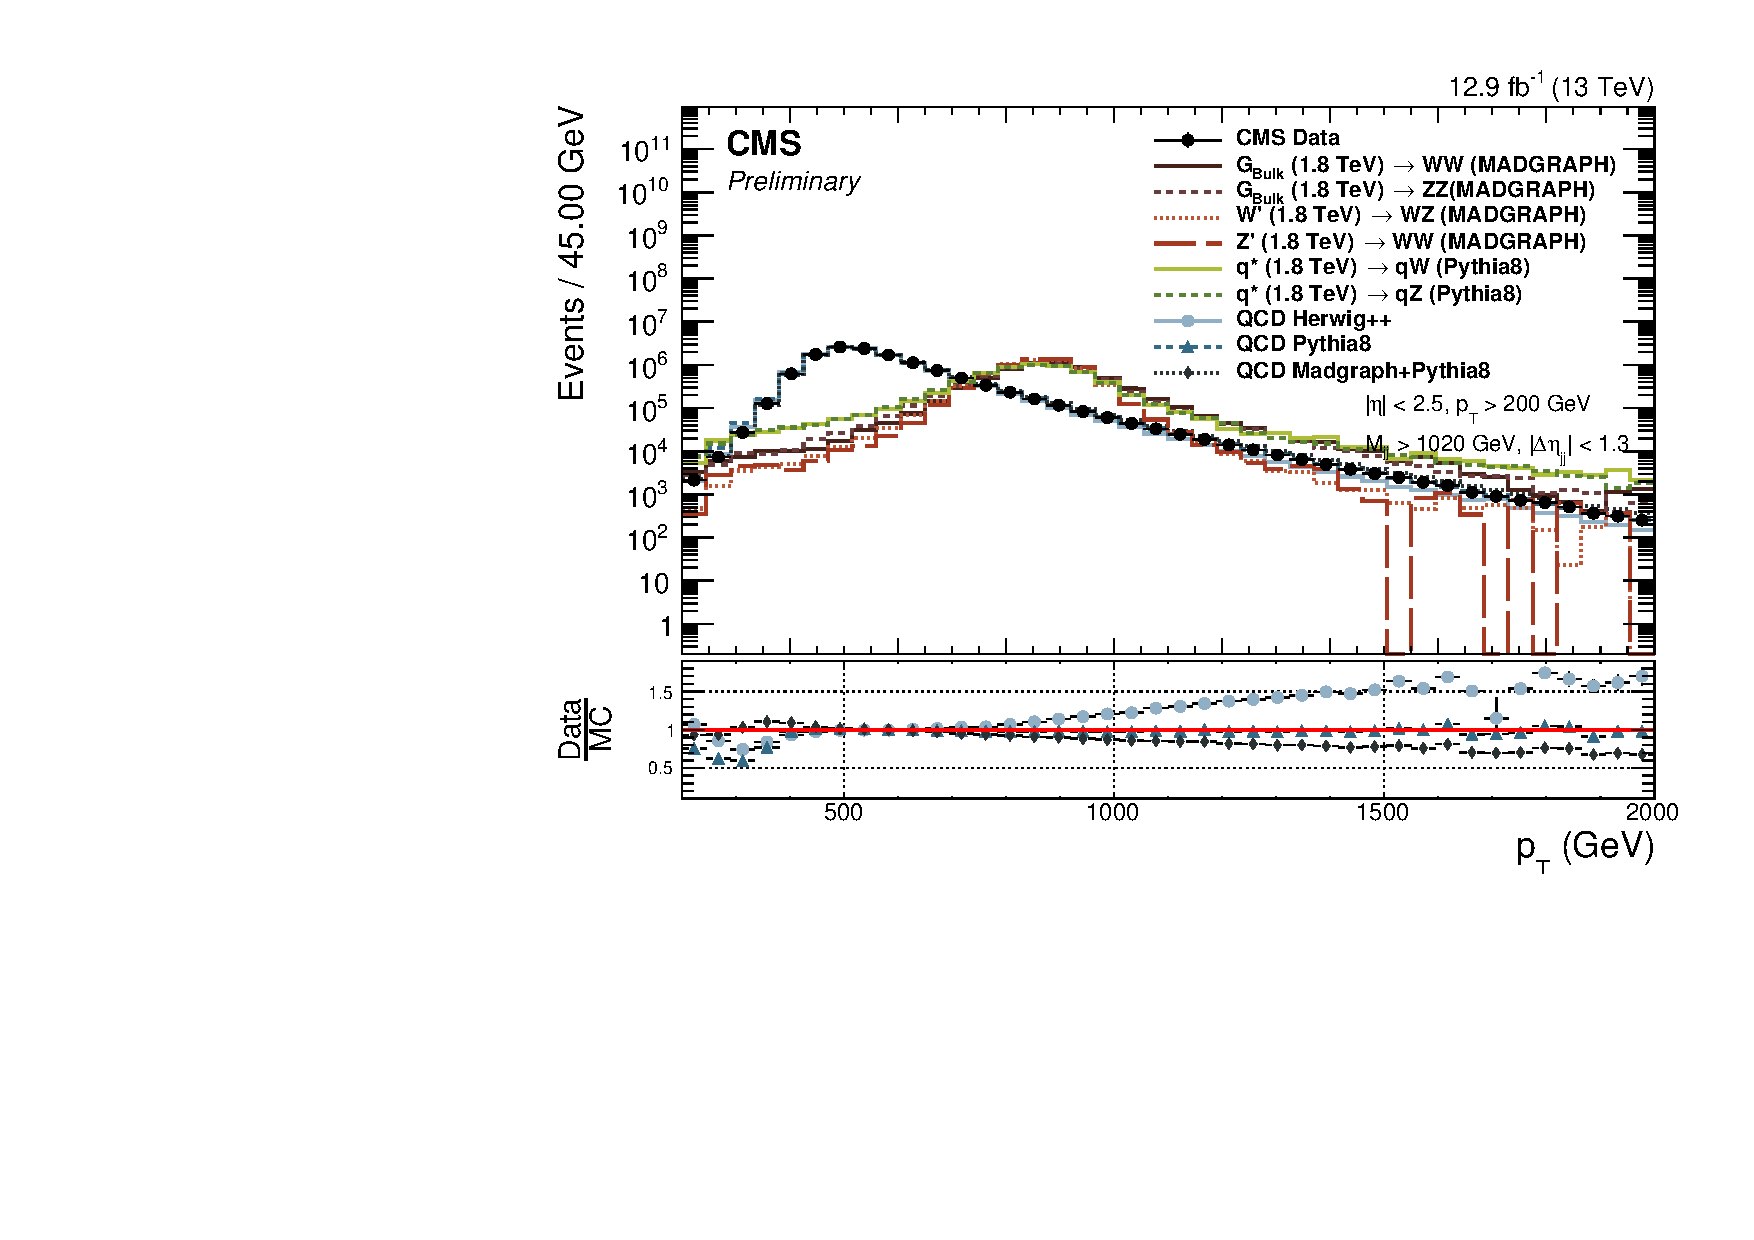
\includegraphics[width=0.49\textwidth]{figures/analysis/search2/AN-16-235/plots/qcdcp_Pt.pdf}
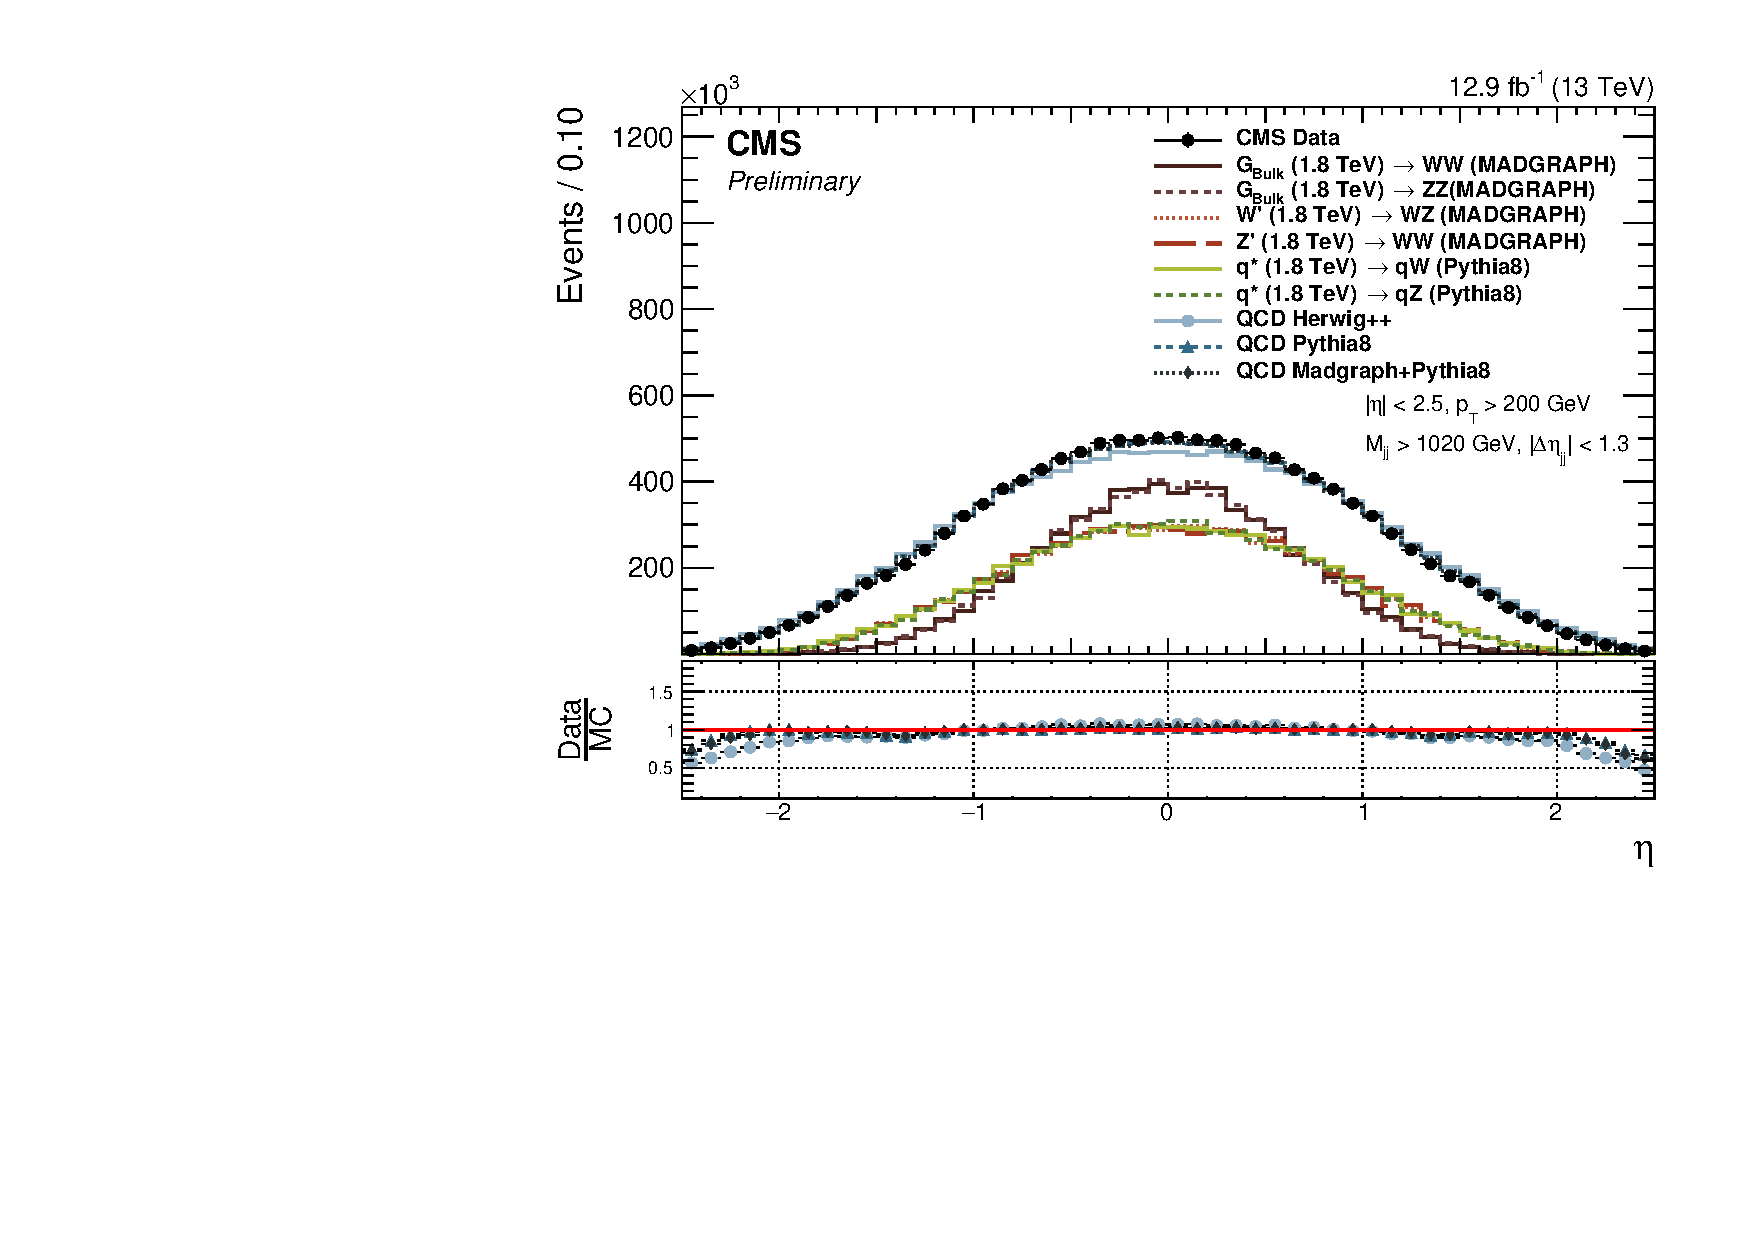
\includegraphics[width=0.49\textwidth]{figures/analysis/search2/AN-16-235/plots/qcdcp_Eta.pdf}\\
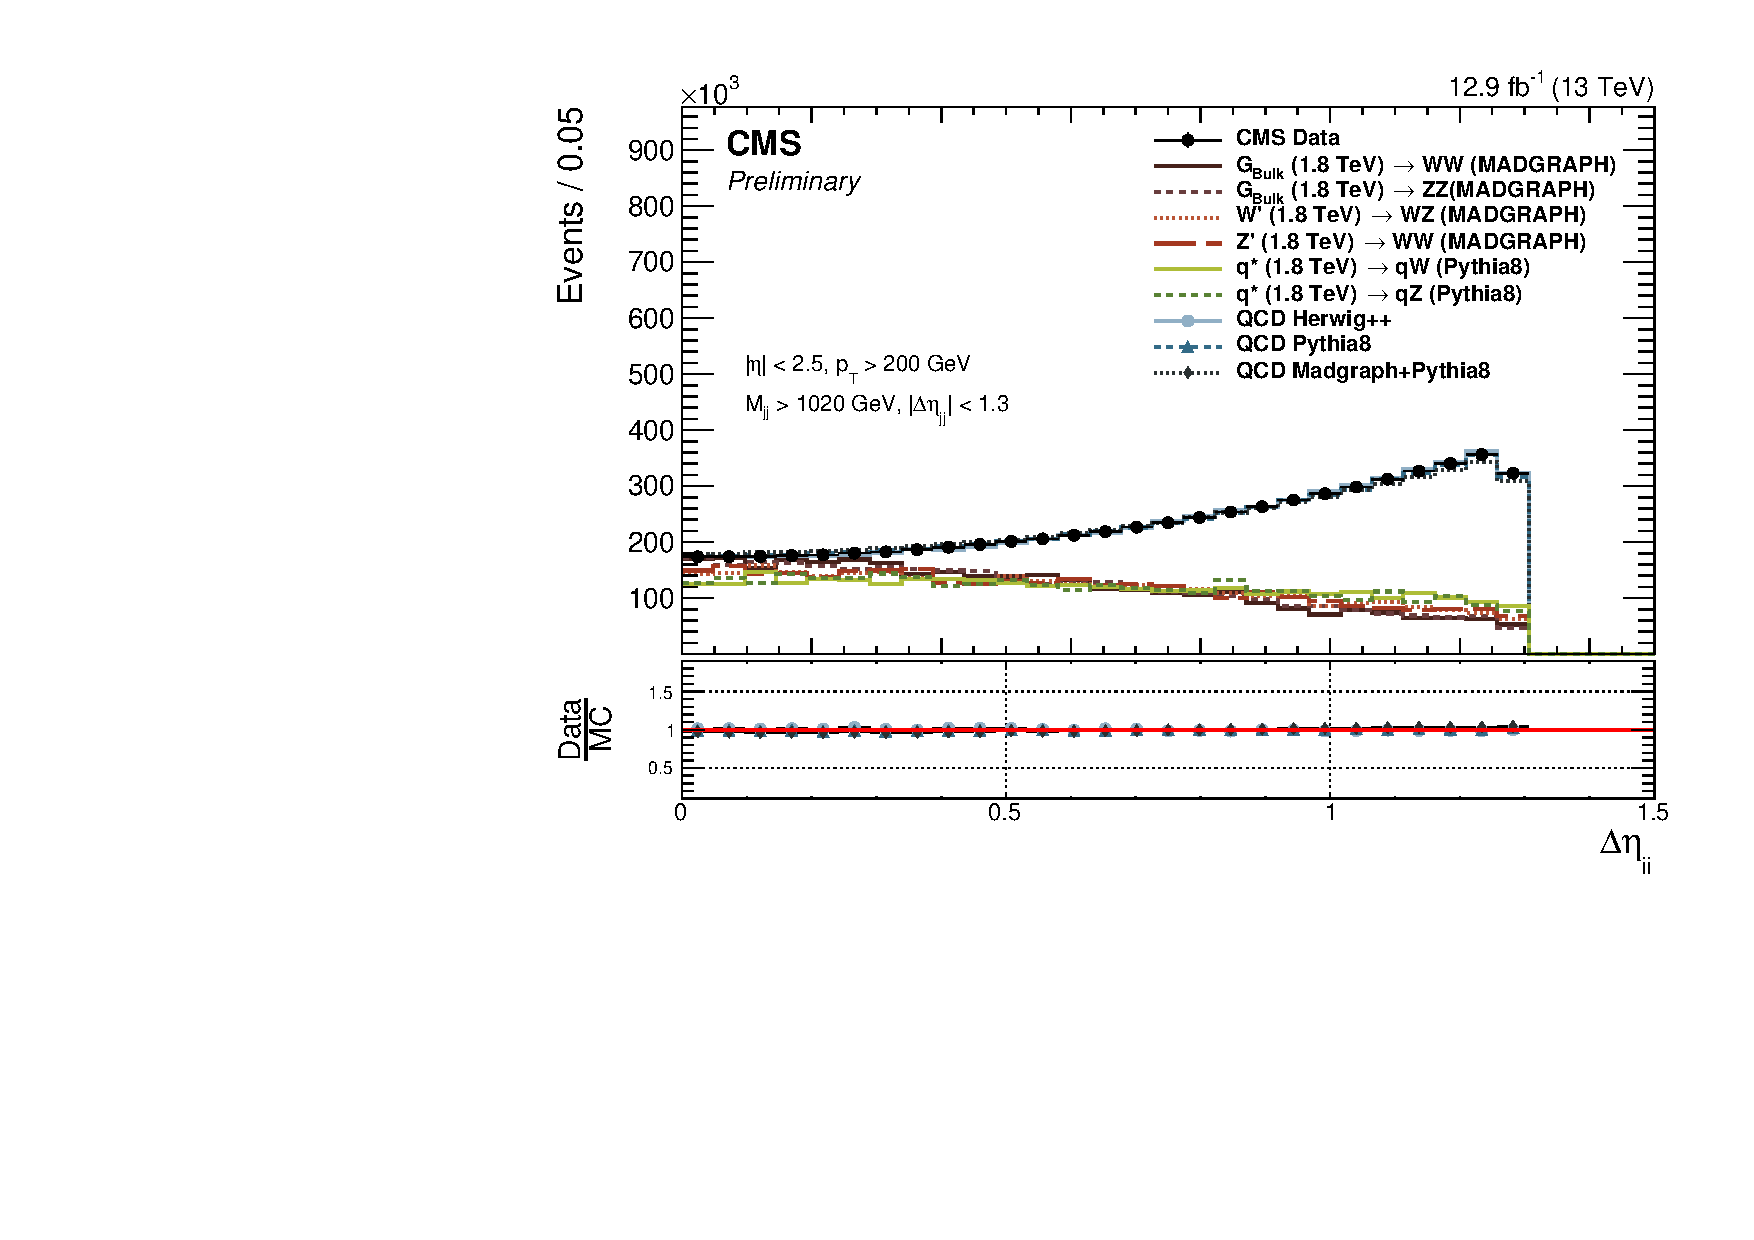
\includegraphics[width=0.49\textwidth]{figures/analysis/search2/AN-16-235/plots/qcdcp_DeltaEta.pdf}
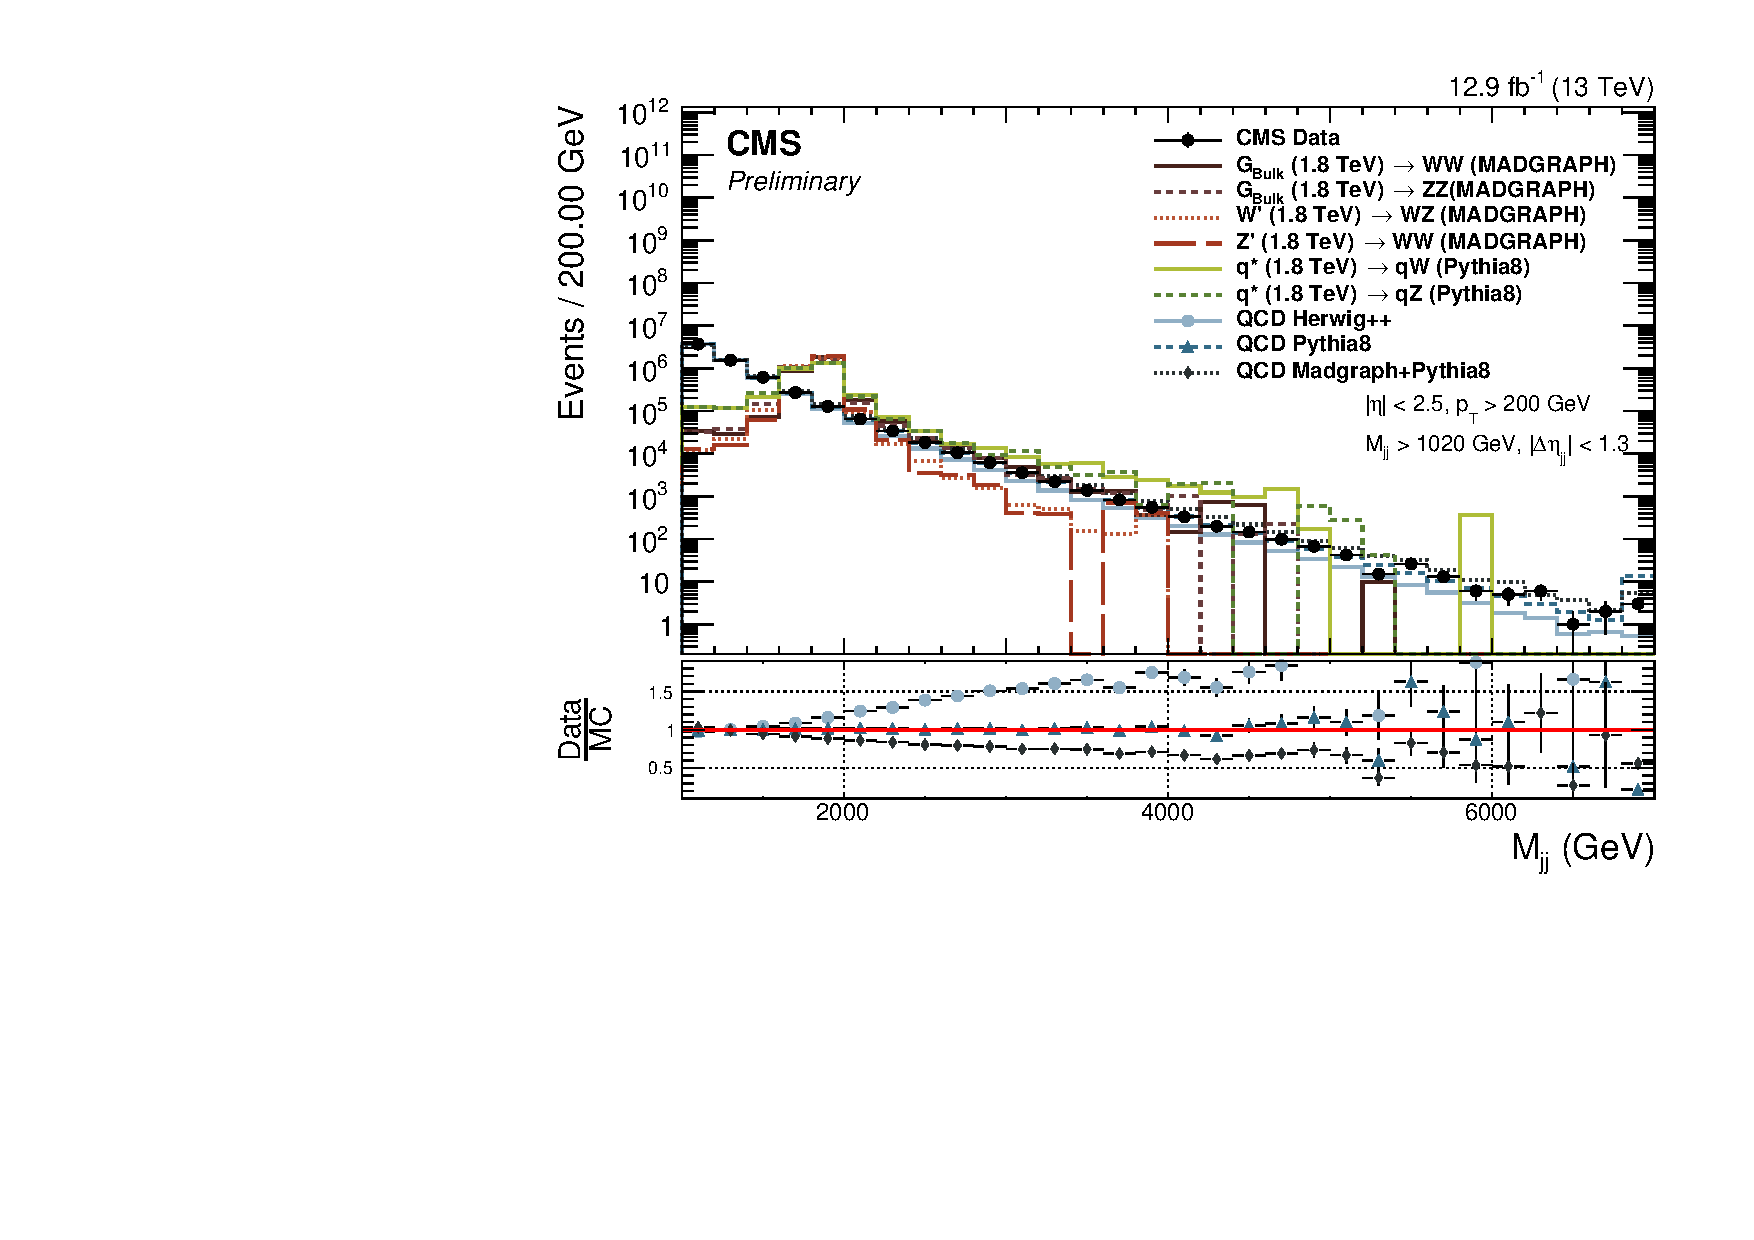
\includegraphics[width=0.49\textwidth]{figures/analysis/search2/AN-16-235/plots/qcdcp_Mjj.pdf}
\caption{Jet \PT{} (top left), $\eta$ (top right), $\Delta \eta_{jj}$ (bottom left) and dijet invariant mass (bottom right) for the two leading jets in the event after loose preselections are applied. The signal is scaled by an arbitrary number.}
\label{fig:searchII:kinematics-all}
\end{figure}
A large difference in slope in the jet \PT and dijet invariant mass spectrum depending on the QCD matrix element or shower generator is observed. Pure \PYTHIA QCD MC describes the data best, while \HERWIG{++} tends to underestimate and \amcatnlo{}+\PYTHIA tends to overestimate the number of high $\PT/\mjj$ jets. Pure \PYTHIA{8} QCD MC is therefore used for all background checks in this analysis.

\clearpage
\section{Developing a new W-tagger}
\label{sec:searchII:puppisoftdrop}
As mentioned in the introduction to this chapter, studies had shown that the PUPPI pileup subtraction algorithm yielded superior resolution on large-cone jet observables like the jet mass. We therefore wanted to check whether the softdrop jet mass, and its observed sensitivity to the underlying event and pileup, would be improved if a better pileup subtraction algorithm was applied pre-clustering.\par
Two interesting observations were made. Softdrop used together with PUPPI pileup subtraction displayed a much smaller \PT-dependent shift than the combination of CHS and softdrop. Figure~\ref{fig:searchII:sdmass} shows the PUPPI softdrop jet mass for W-jets from a 1 \TeV resonance, corresponding to a jet $\PT\sim 500 \GeV$, and a 4 \TeV resonance, corresponding to a jet $\PT\sim 2 \TeV$, exhibiting the desired reduced \PT dependence on jet mass scale. 
\begin{figure}[h!]
\centering
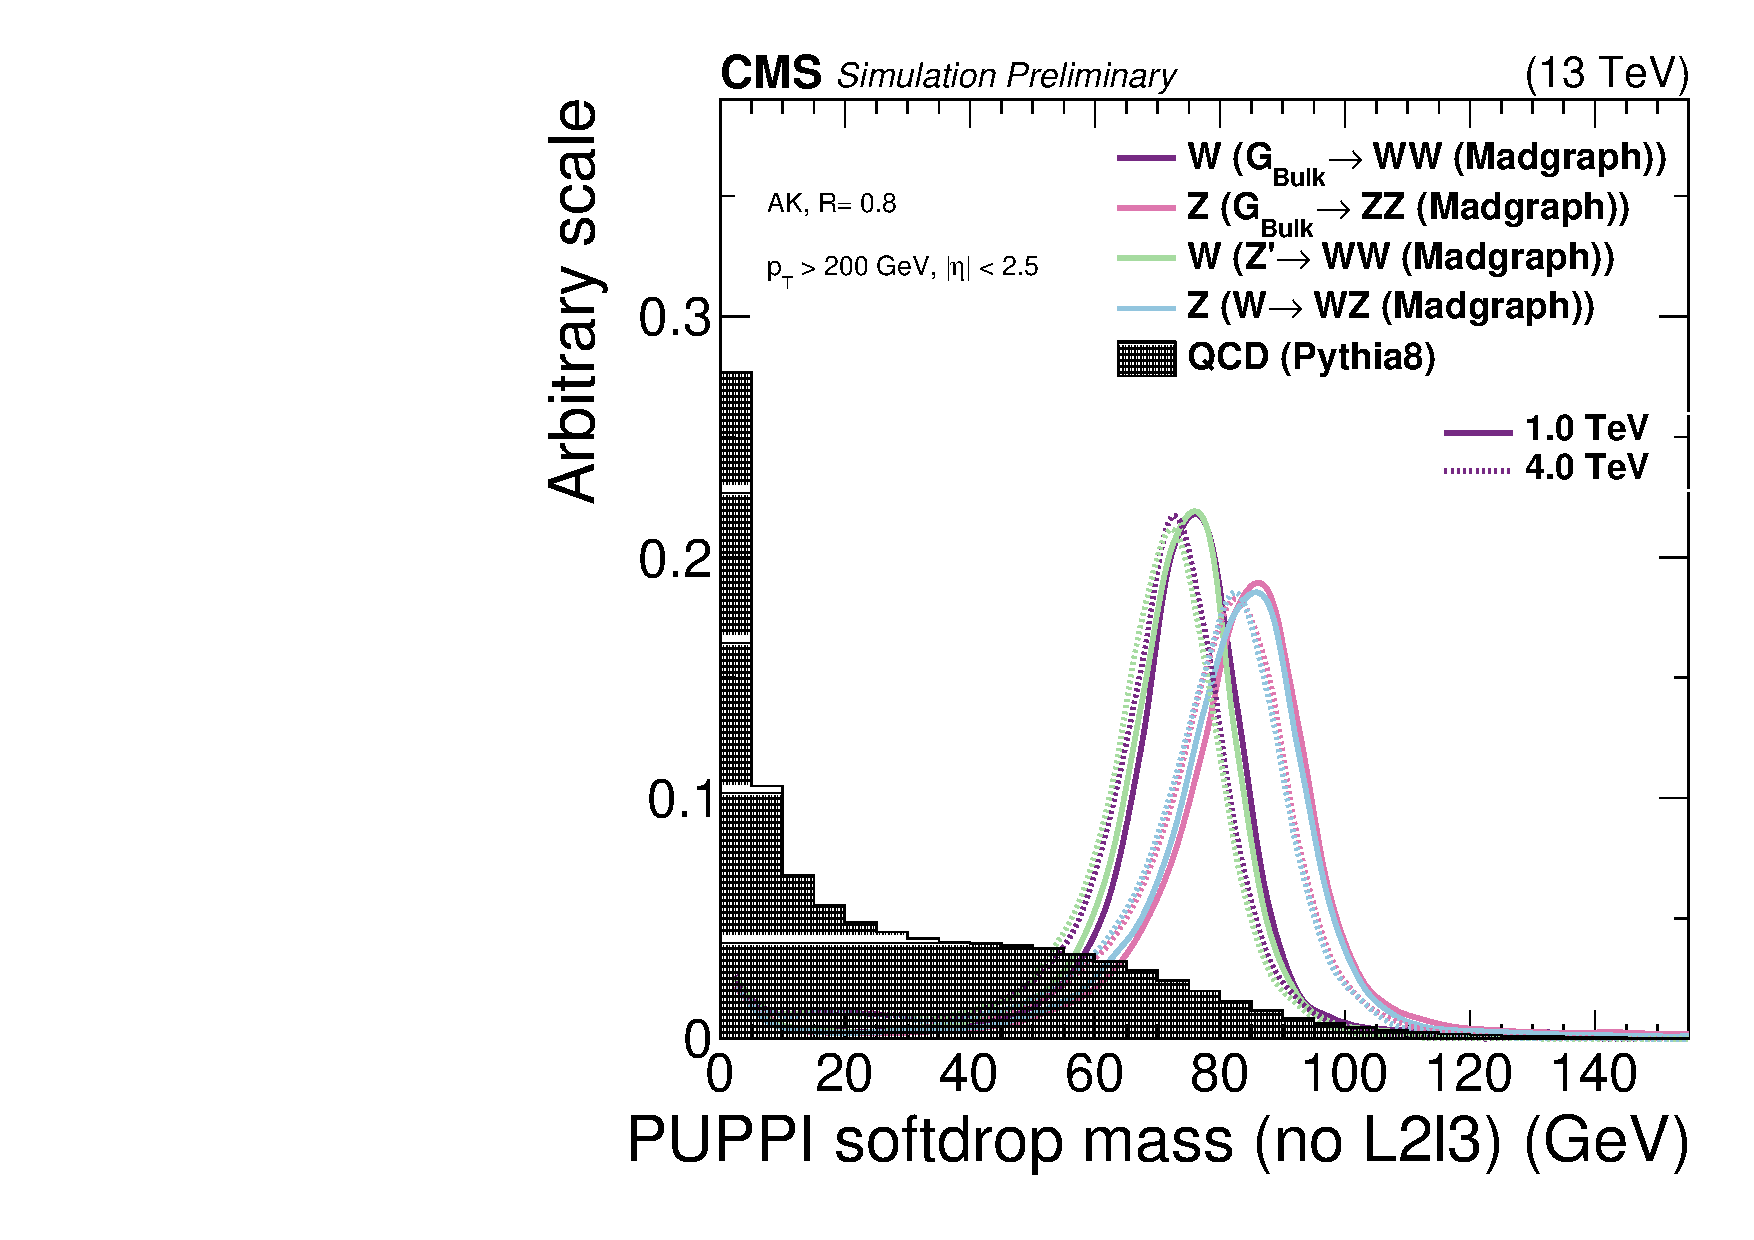
\includegraphics[width=0.49\textwidth]{figures/analysis/search2/AN-16-235/plots/gen_SoftdropMassUnCorr.pdf}
\caption{The PUPPI softdrop jet mass distribution for W boson jets coming from a 1 and 4 TeV resonance assuming different signal hypothesis. The QCD multijet background is shown in gray. No jet energy corrections have been applied to the jets.}
\label{fig:searchII:sdmass}
\end{figure}
However, when applying the recommended L2 and L3 jet energy corrections (see Section~\ref{sec:objreco:jec}) to the jet groomed mass, a strong \PT dependent shift is re-introduced. This effect is not present for the pruned jet mass. Figure~\ref{fig:searchII:wtagmass} shows the softdrop (top left) and pruned (top right) jet mass distributions with recommended L2L3 corrections applied. Here, the PUPPI softdrop jet mass shift as a function of \PT is significantly increased with respect to what was observed for the uncorrected mass, while the CHS pruned jet mass remains stable. This points to the PUPPI jet energy corrections not being optimal for PUPPI soft-dropped jets. Indeed, there is no reason to expect the CMS JEC corrections to work for groomed jets at all as they were derived from un-groomed PUPPI or CHS jets. The fact that they work well for CHS pruned jets is not a given. The jet energy corrections derived for CHS and PUPPI jets as a function of jet \PT are shown in the bottom plot in Figure~\ref{fig:searchII:wtagmass}. A significant slope in JEC as a function of \PT is measured for PUPPI, while not present for CHS.
\begin{figure}[h!]
\centering
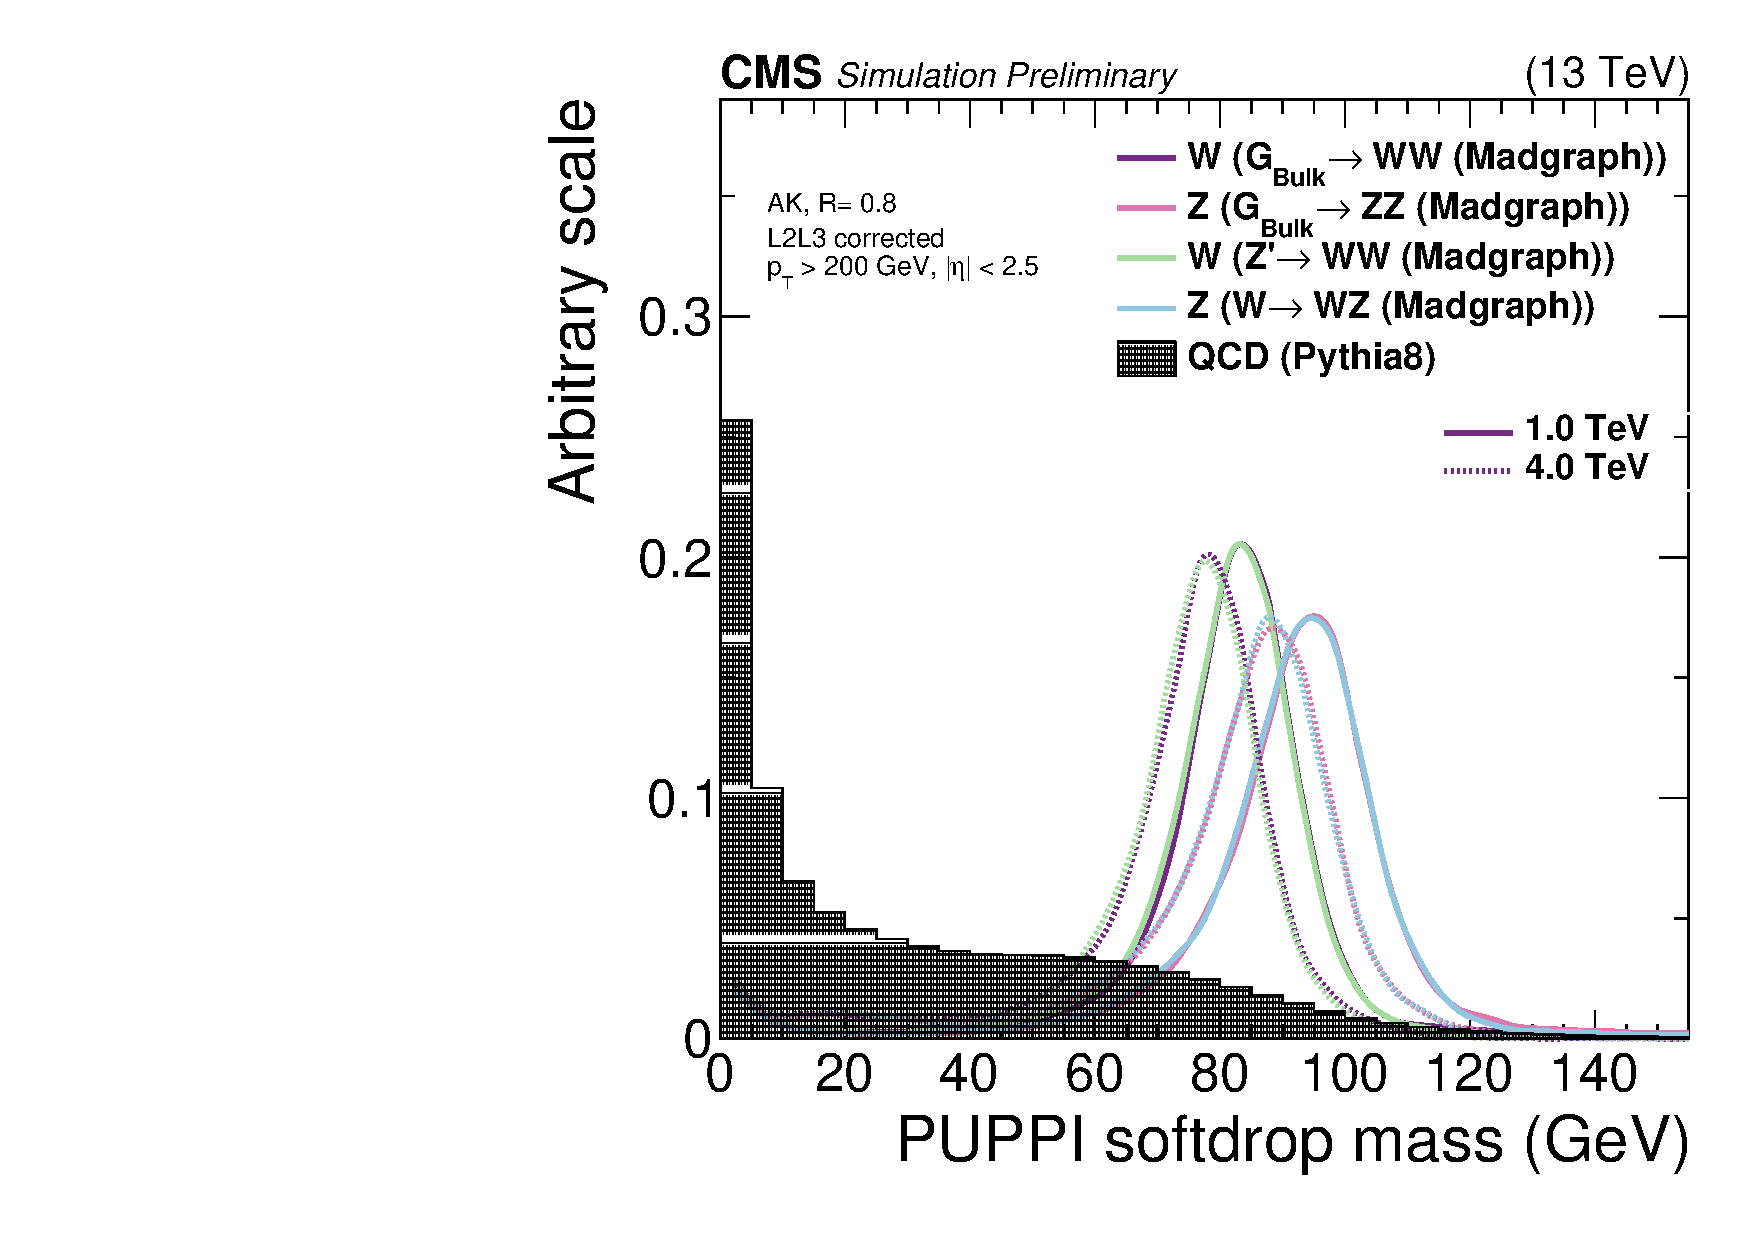
\includegraphics[width=0.4\textwidth]{figures/analysis/search2/AN-16-235/plots/gen_SoftdropMass.pdf}
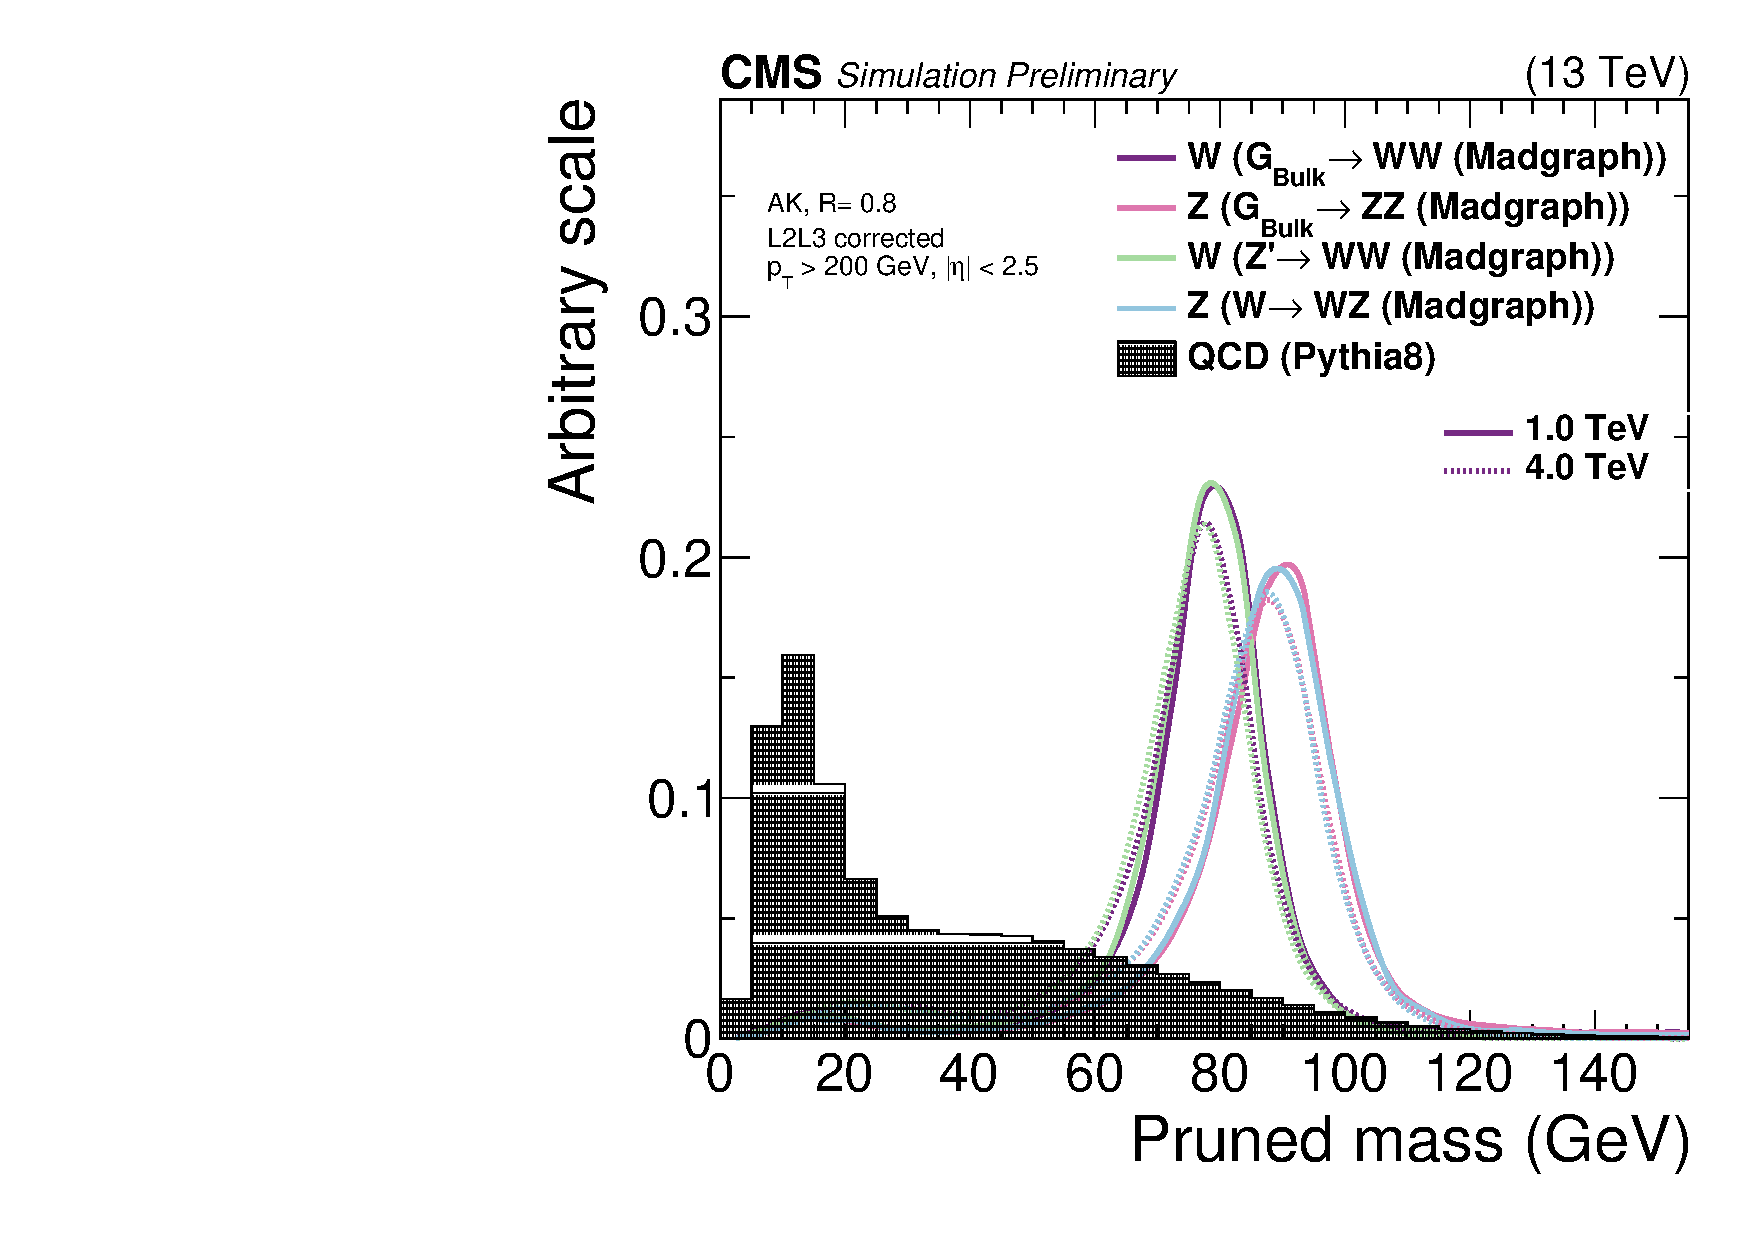
\includegraphics[width=0.4\textwidth]{figures/analysis/search2/AN-16-235/plots/gen_PrunedMass.pdf}\\
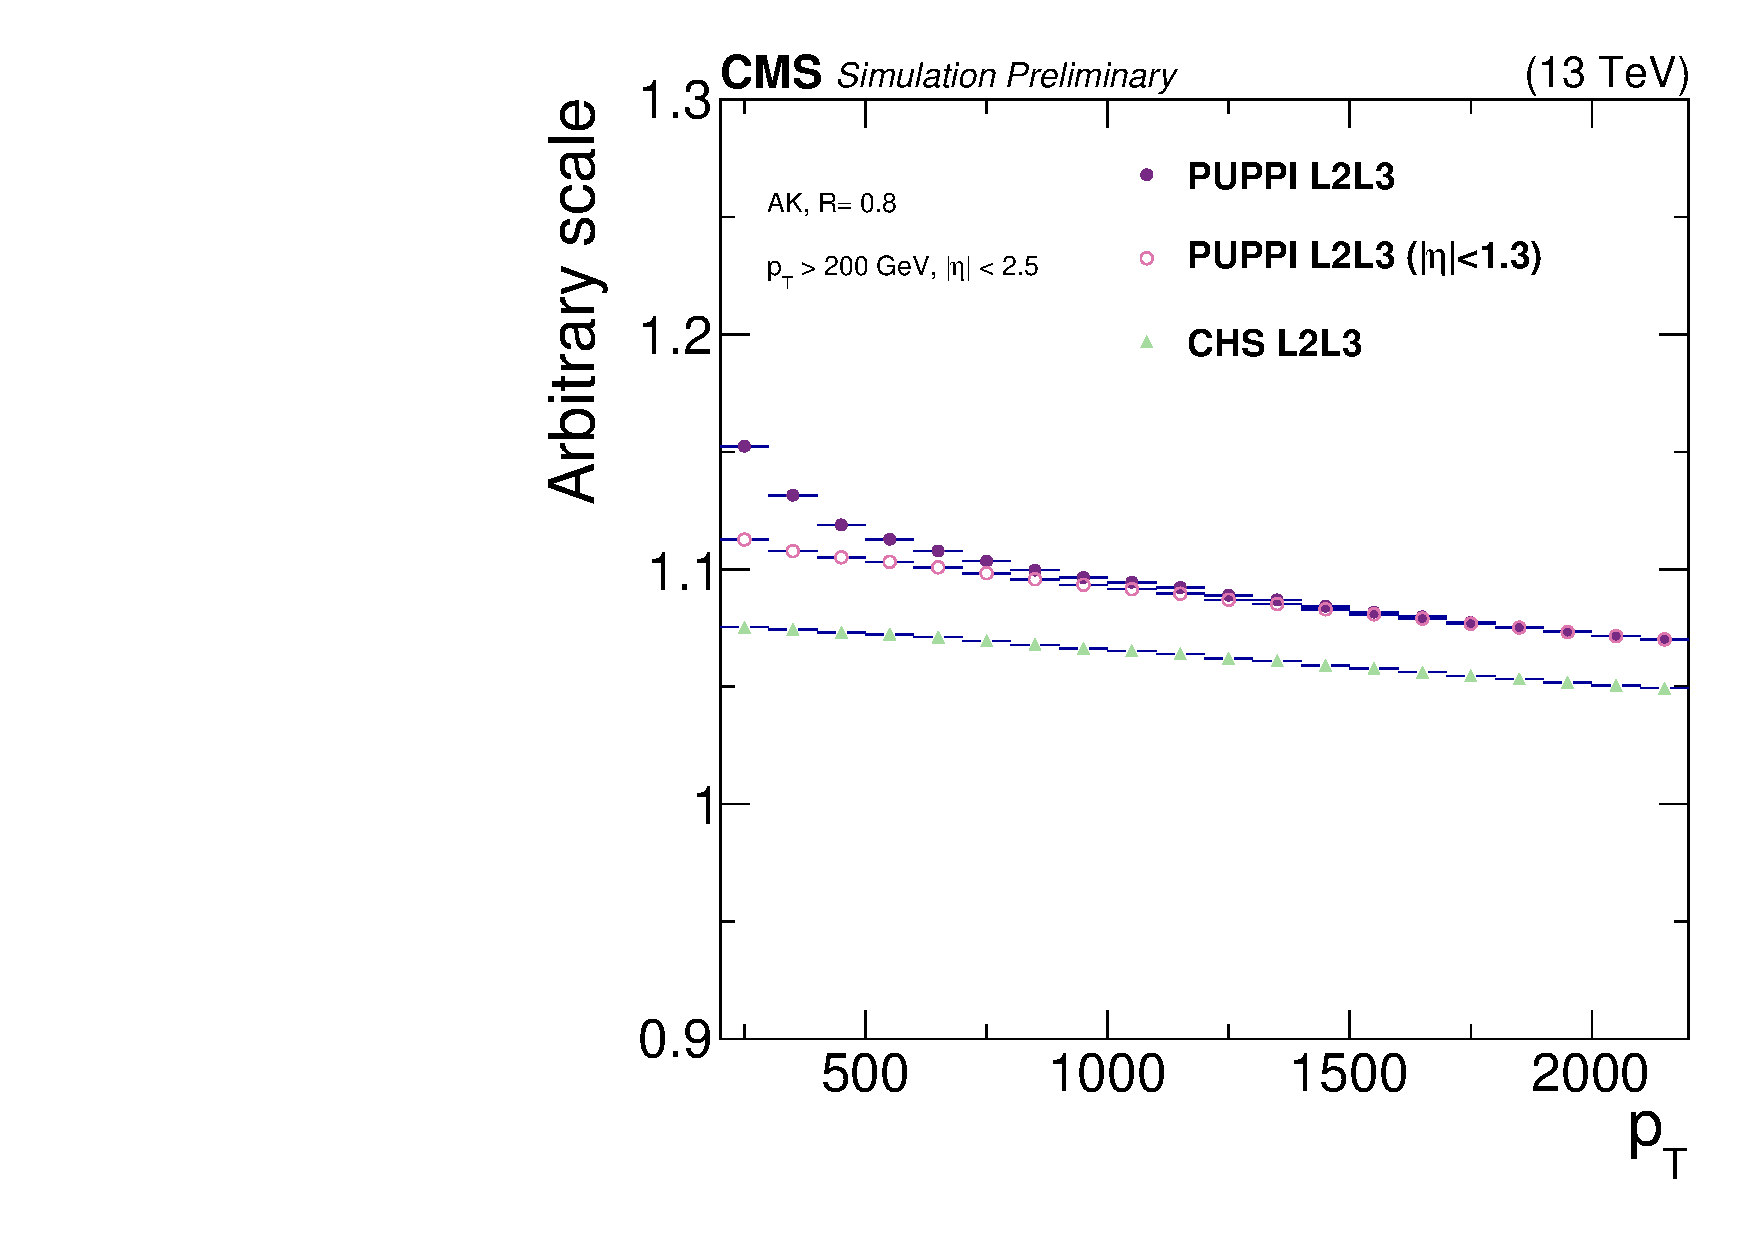
\includegraphics[width=0.4\textwidth]{figures/analysis/search2/AN-16-235/plots/JECvsPT.pdf}
\caption{Top: PUPPI softdrop jet mass distribution (top left) and pruned jet mass distribution (top right) with L2 and L3 corrections applied. Bottom: The projection of CHS and PUPPI jet energy corrections versus jet \PT.}
\label{fig:searchII:wtagmass}
\end{figure}

\subsection{Dedicated PUPPI softdrop jet mass corrections}
\label{sec:searchII:masscorr}
In order to remove the PUPPI softdrop jet mass dependence on jet \PT, all jet energy corrections to the softdrop jet mass are removed. However, this still leaves a residual \PT-dependent shift and, in addition, the uncorrected mass does not peak near the correct W-mass of 80.4~\GeV. Figure~\ref{fig:searchII:UncorrSD} shows the mean of a Gaussian fit to the uncorrected PUPPI softdrop mass as a function of jet $\pt$ in two different $\eta$ bins (smaller or greater than $|\eta|=1.3$) for W-jets coming from a Bulk Graviton signal sample. A mass shift both as a function of $\eta$ and \PT is observed, together with an average mean shifted significantly lower than the W boson mass.
\begin{figure}[h!]
\centering
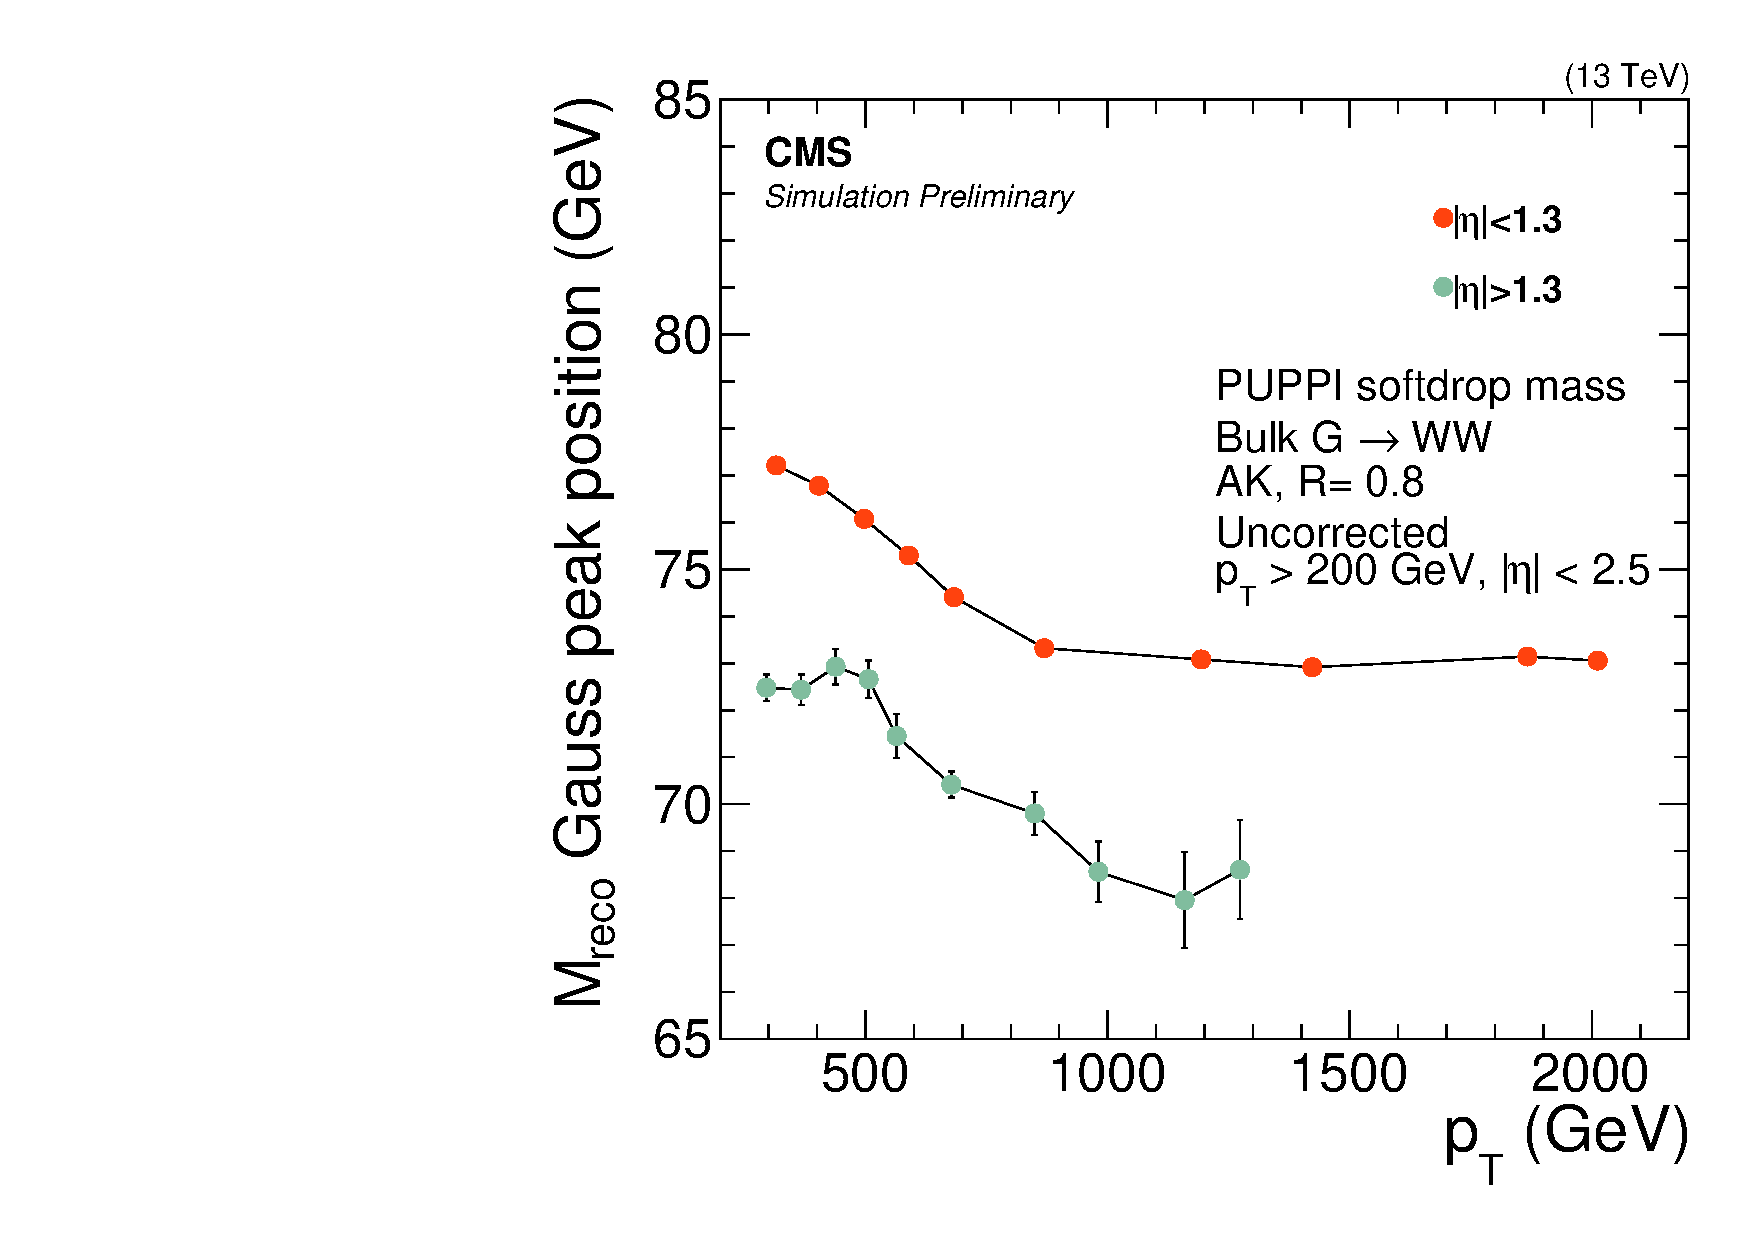
\includegraphics[width=0.49\textwidth]{figures/analysis/search2/AN-16-235/plots/RecoPuppiSoftdropMass_vspt.pdf}
\caption{The mean of a Gaussian fit to the W-jet PUPPI softdrop mass peak as a function of jet \PT in two different $\eta$ bins (smaller or greater than $|\eta|=1.3$). No jet energy corrections have been applied to the softdrop mass.}
\label{fig:searchII:UncorrSD}
\end{figure}
In order to use PUPPI softdrop for W tagging, we therefore derive dedicated jet-mass corrections to compensate for two factors: a generator-level \PT-dependence, as first observed in Section~\ref{sec:searchI:wtagging}, and a reconstruction-level \PT- and $\eta$-dependence, most likely due to calibration (recall, the PUPPI jet energy corrections have been removed). Figure~\ref{fig:searchII:sdmassshifts} shows the mean of the generated softdrop jet mass (left) and the normalized difference in reconstructed and generated softdrop jet mass (right) as a function of jet \PT. The shift in generated softdrop mass at lower \PT is of the order of 2-3$\%$ while the difference between reconstructed and generated softdrop mass is a 5-10$\%$ effect.
\begin{figure}[h!]
\centering
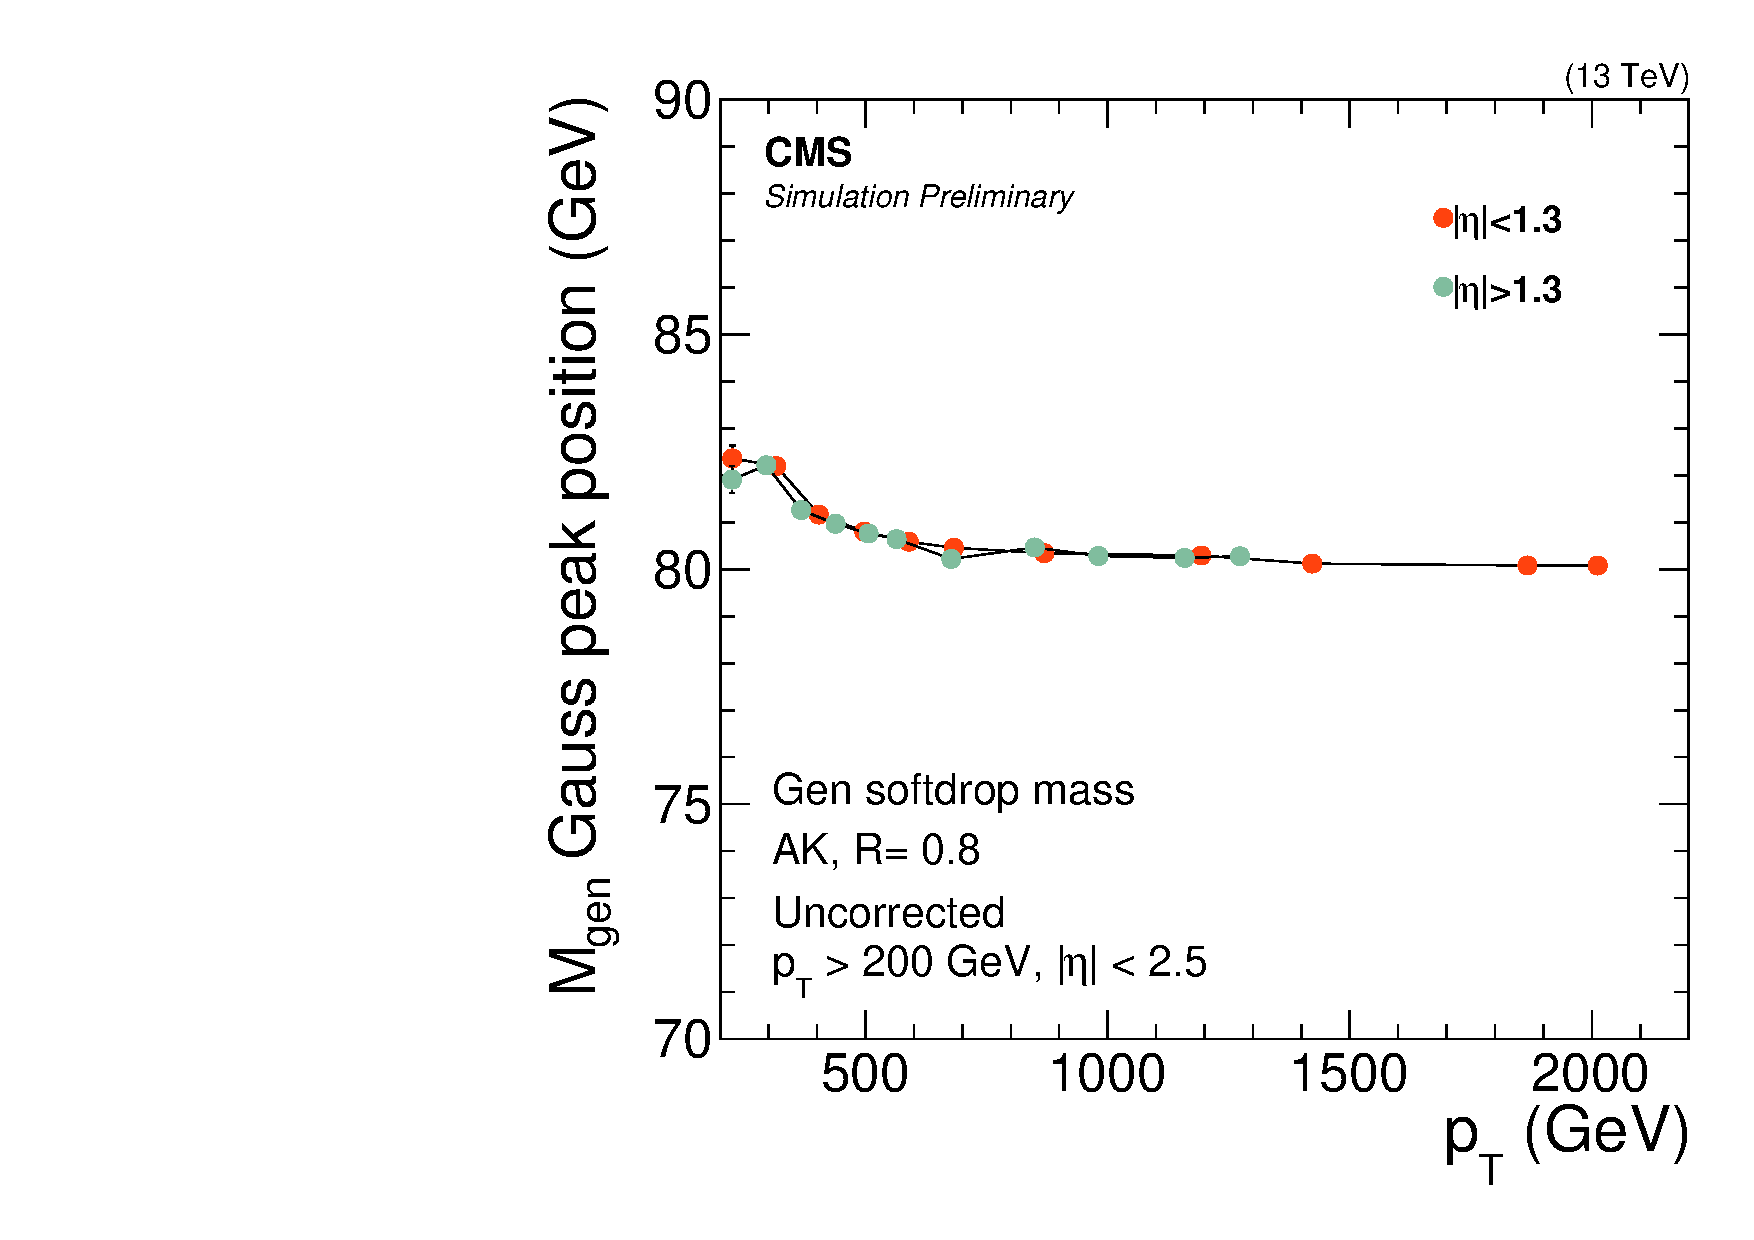
\includegraphics[width=0.49\textwidth]{figures/analysis/search2/AN-16-235/plots/GenSoftdropMass_vspt.pdf}
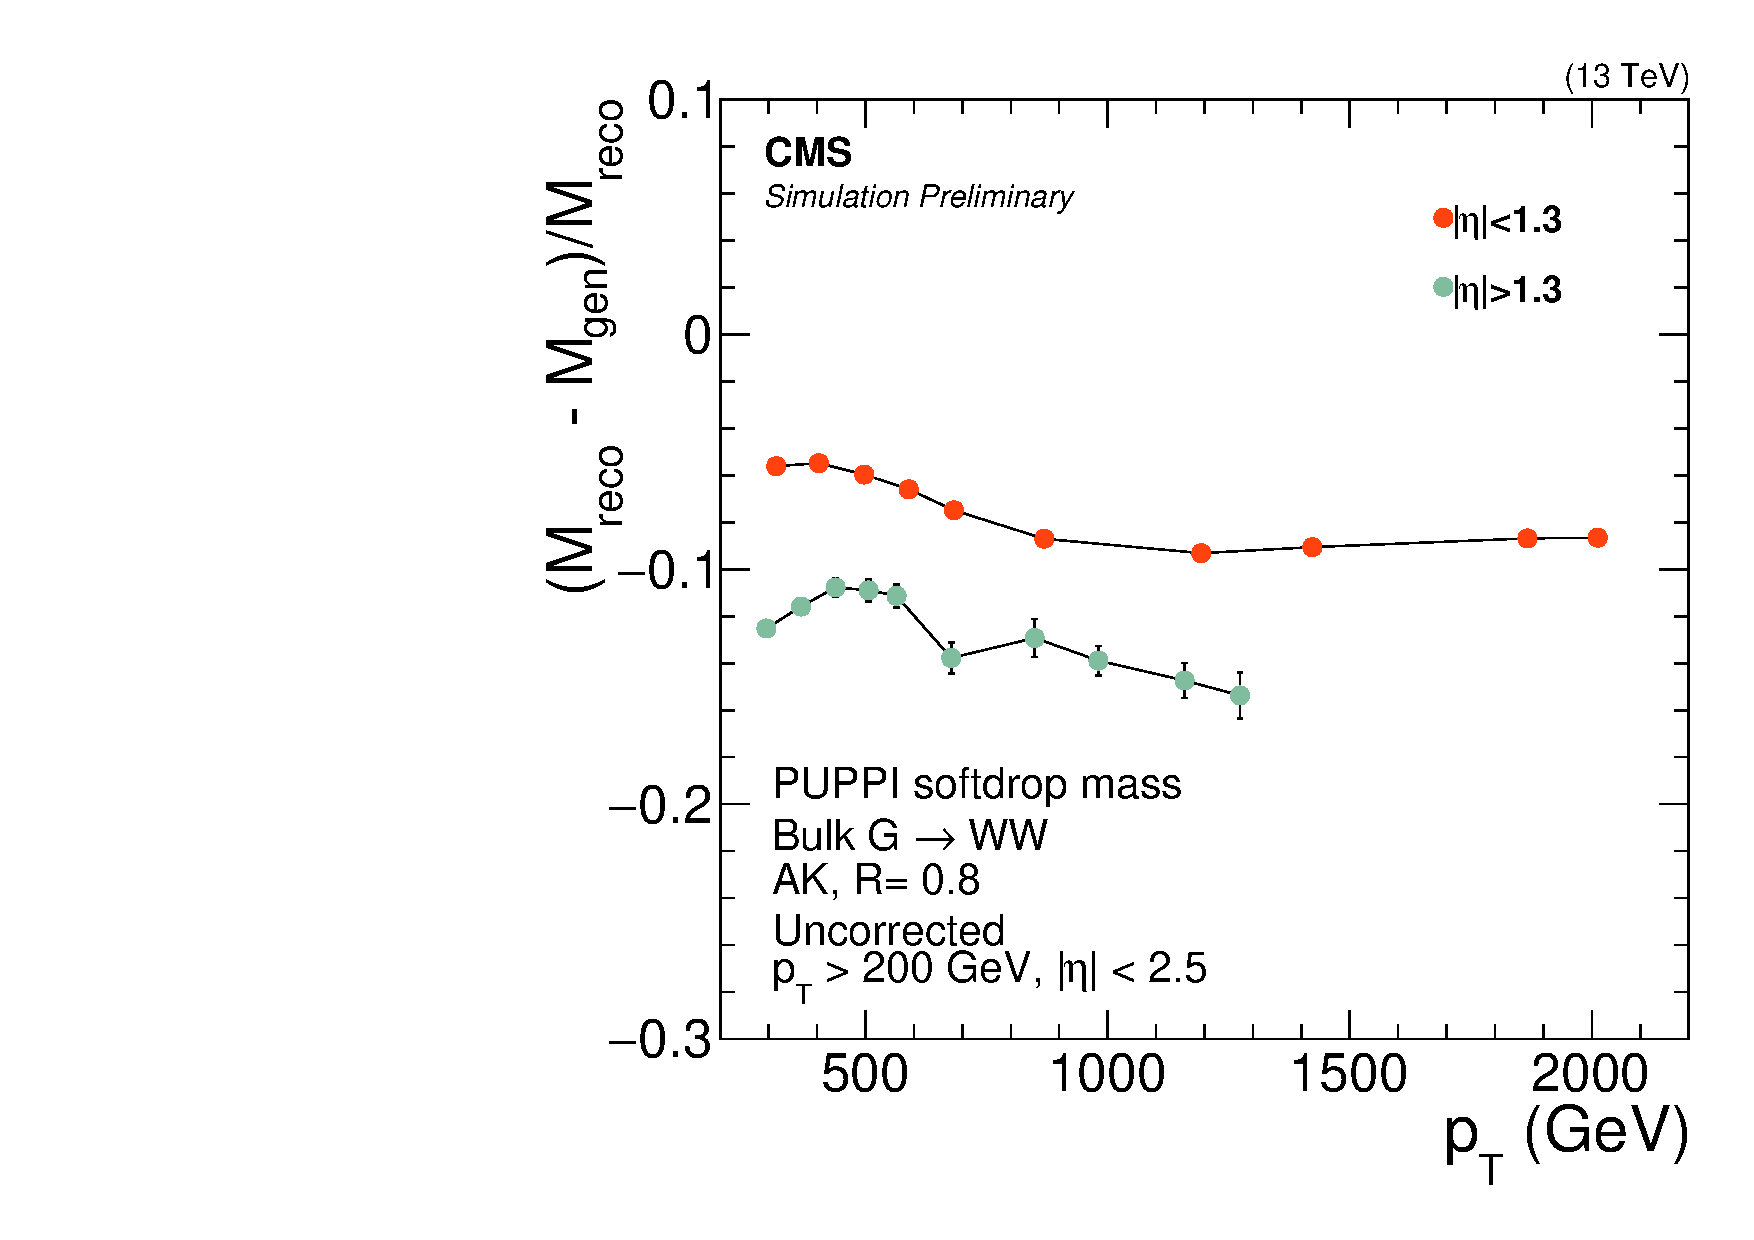
\includegraphics[width=0.49\textwidth]{figures/analysis/search2/AN-16-235/plots/MassShift_vspt.pdf}
\caption{The mean of the fitted generator level W-jet softdrop mass distribution as a function of jet $\pt$ (left) and the normalized difference in reconstructed and generated softdrop jet mass (right).}
\label{fig:searchII:sdmassshifts}
\end{figure}
The mass shift introduced at generator-level is corrected by a fit to $\rm{M_{PDG}/M_{GEN}}$ as a function of jet \PT, where $\rm{M_{PDG}}=80.4~\GeV$ and $\rm{M_{GEN}}$ is the fitted mean of the generator-level mass as shown in the left plot in Figure~\ref{fig:searchII:sdmassshifts}. To correct for the residual shift between generated and reconstructed softdrop mass, a fit to $\rm{(M_{RECO}-M_{GEN})/M_{RECO}}$, where $\rm{M_{RECO}}$ is the reconstructed mass shown in the right plot in Figure~\ref{fig:searchII:sdmassshifts} and $\rm{M_{GEN}}$ is as defined above, as a function of jet \PT in two $\eta$ bins (smaller or greater than $|\eta|=1.3$) is performed.
Polynomial fit functions of the following forms are used:
\begin{align*} 
% w(\pt) &=  [0]+[1]*pow(x*[2],-[3] \\
w(\pt) &=  A  +B(x^{2})^{-C}          &\sim\textrm{``gen correction''} and\\
w(\pt) &=  A  +Bx+Cx^2+Dx^3+Ex^4+Fx^5 &\sim\textrm{``reco correction''}. 
\end{align*}
The distribution and corresponding parametrization of the two corrections is shown in Figure~\ref{fig:jmcfits} for the "gen correction" (left) and "reco correction" (right).
\begin{figure}[h!]
\centering
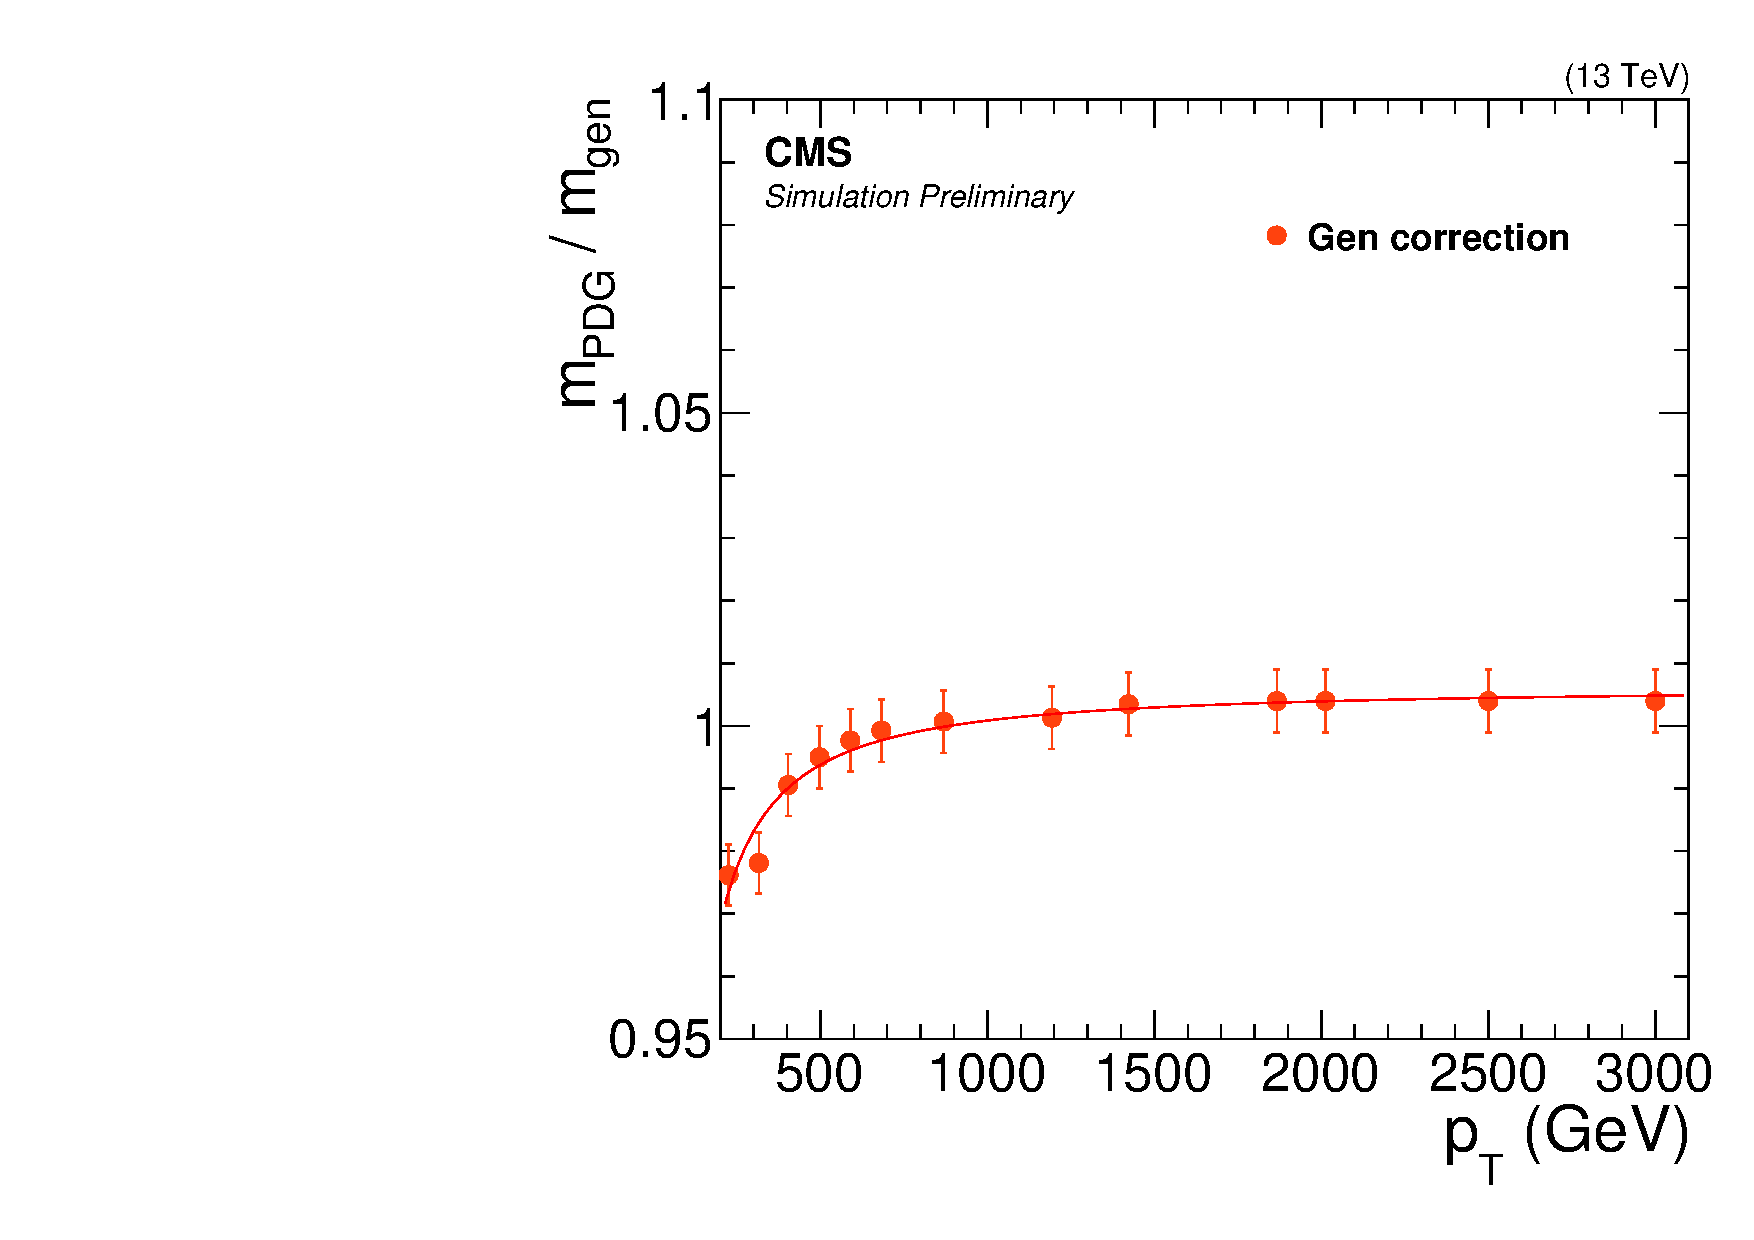
\includegraphics[width=0.45\textwidth]{figures/analysis/search2/AN-16-235/plots/JMC_fit_gen.pdf}
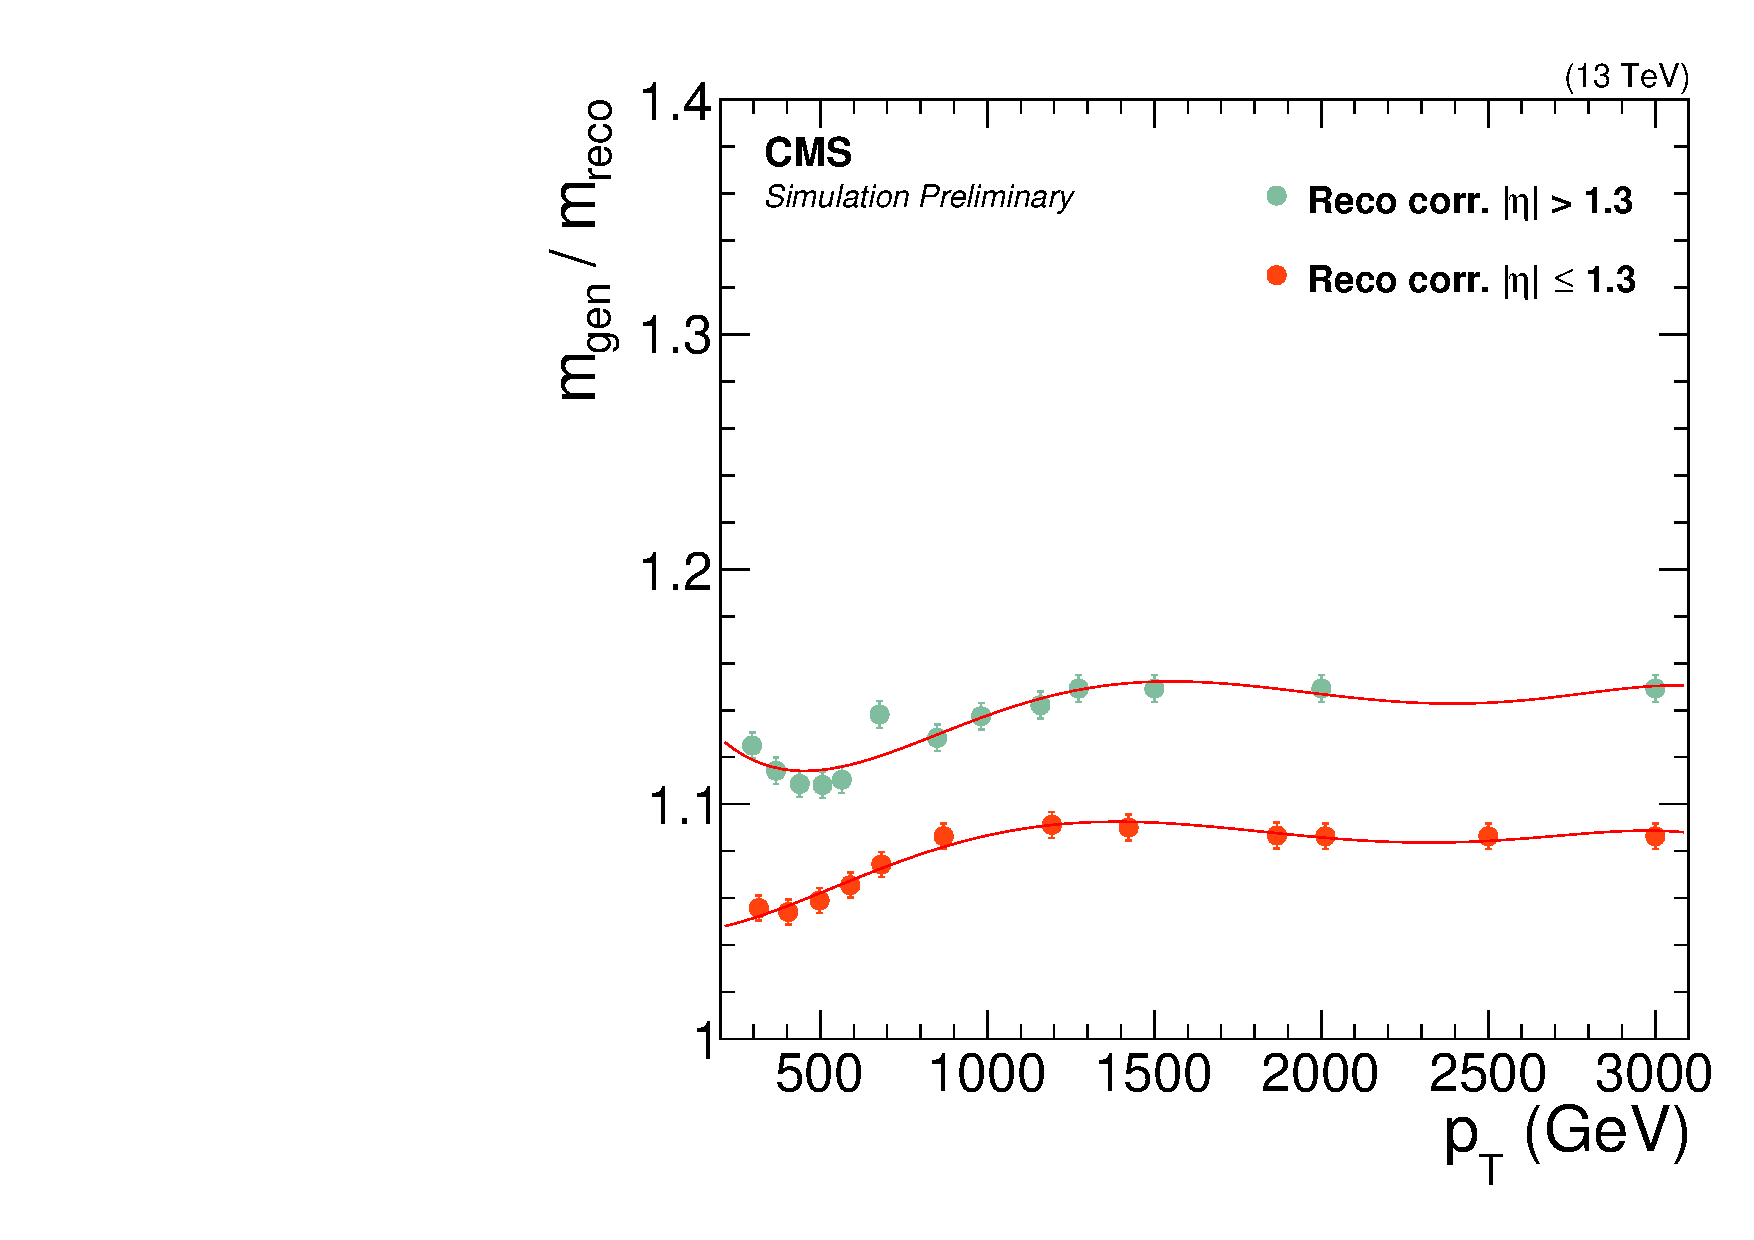
\includegraphics[width=0.45\textwidth]{figures/analysis/search2/AN-16-235/plots/JMC_fit_reco.pdf}
\caption{Left: fit to $\rm{M_{PDG}/M_{GEN}}$ as a function of jet $\pt$, where $\rm{M_{PDG}}=80.4~\GeV$ and $\rm{M_{GEN}}$ is the fitted mean of the generator level mass. Right: fit to $\rm{(M_{RECO}-M_{GEN})/M_{RECO}}$, where $\rm{M_{RECO}}$ is the reconstructed softdrop mass, as a function of jet $\pt$ in two $\eta$ bins.}
\label{fig:jmcfits}
\end{figure}
The two corrections are then applied to the uncorrected PUPPI softdrop mass both in data and in MC as
\begin{equation}
M_{SD}=M_{\rm{SD, uncorr}} \times \rm{w_{GEN}} \times \rm{w_{RECO}}
\end{equation}
where $w_{GEN}$ and $w_{RECO}$ correspond to the generator and reconstructed level corrections, respectively, and $M_{\rm{SD, uncorr}}$ is the uncorrected PUPPI softdrop mass. \par
A closure test is performed in order to check that the corrected PUPPI softdrop W-jet mass peaks at 80.4 \GeV and is stable with respect to the jet \PT and $\eta$. The fitted mean of the corrected PUPPI softdrop mass peak as a function of jet \PT in two different $\eta$ bins is shown in Figure~\ref{fig:searchII:wtagclosure}. Good closure is observed, with the corrected mass peaking around 80 GeV independent of the jet $\pt$ and $\eta$. The PUPPI softdrop jet mass peak for W, Z, and Higgs boson jets from different signal samples after jet mass corrections have been applied is shown in Figure~\ref{fig:search2:corrMass}, for resonances with a mass of 1 and 4 TeV. The corrections yield a mass stable with \PT, peaking around the boson mass, for all three boson-jets under consideration. 
\begin{figure}[h!]
\centering
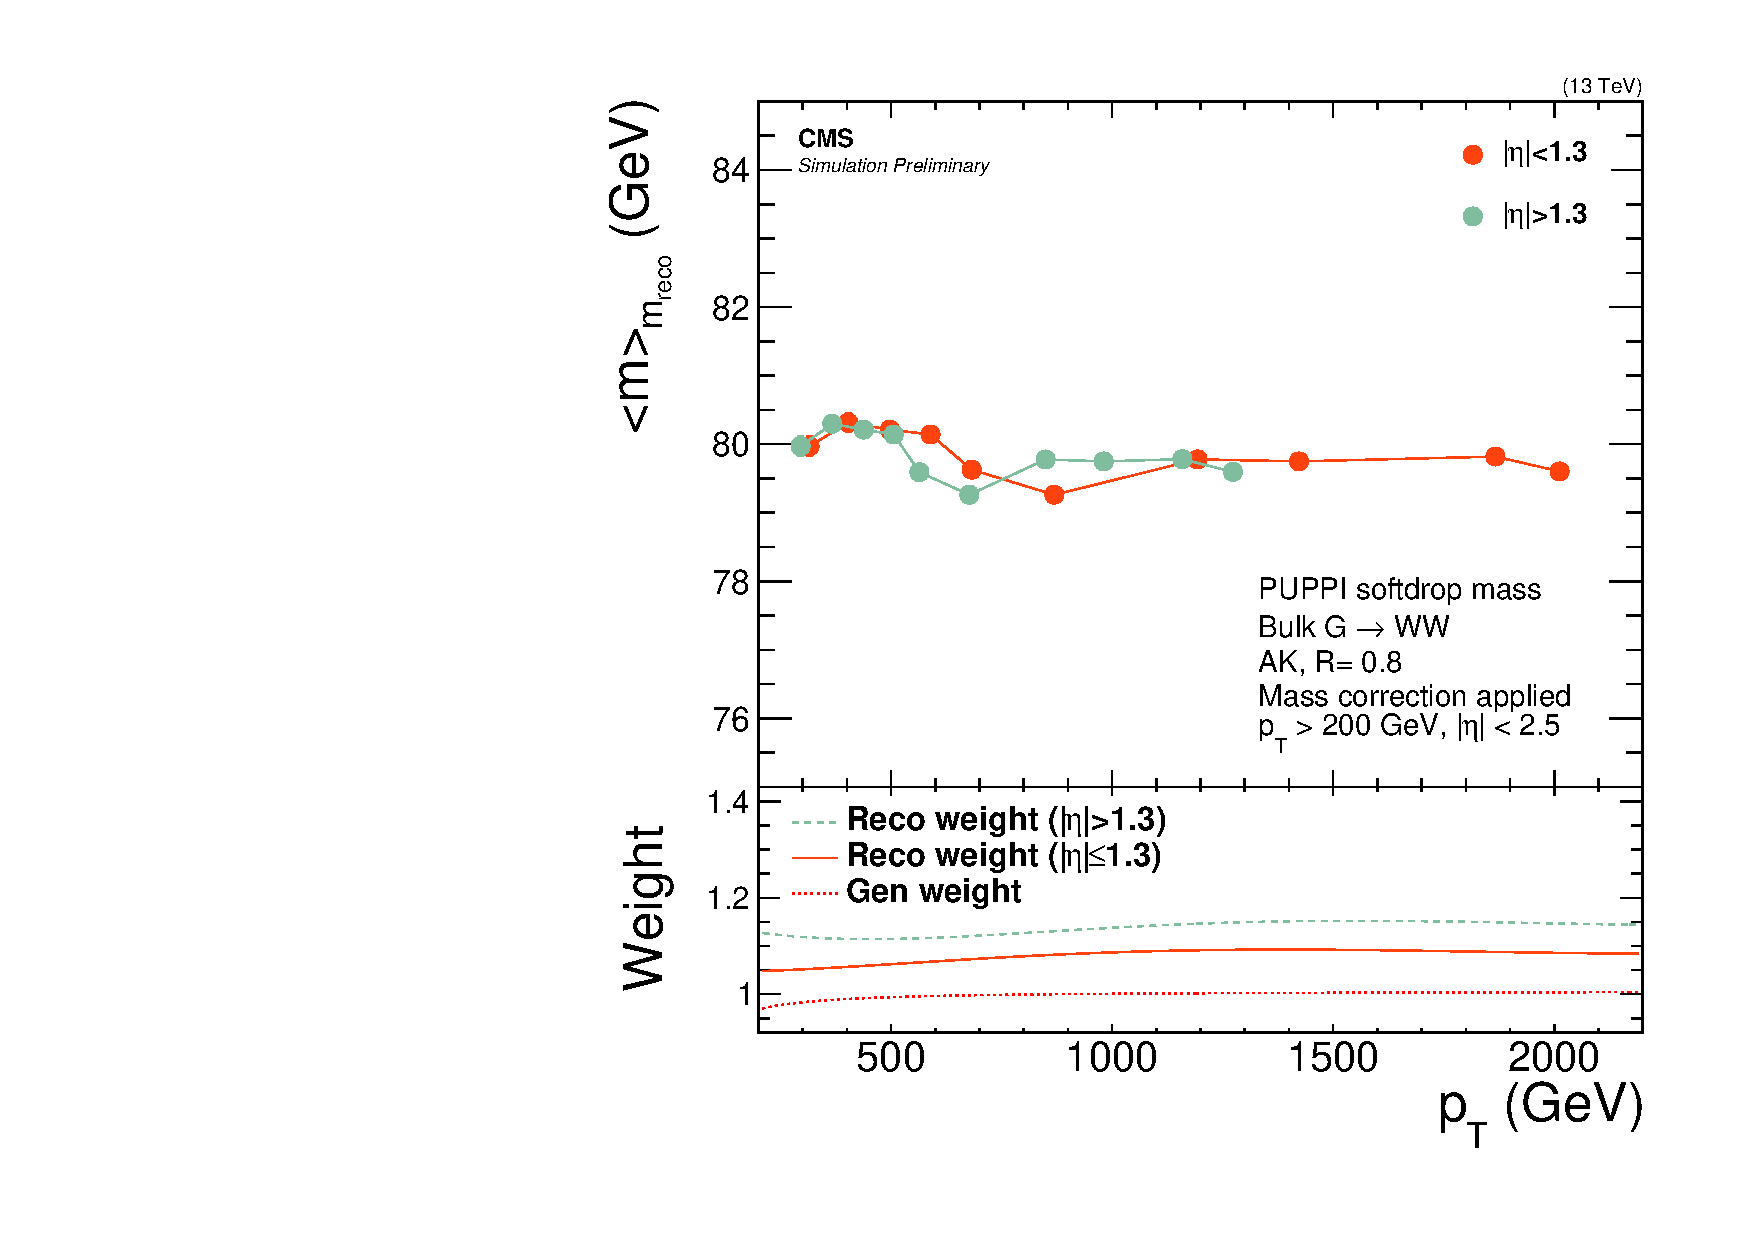
\includegraphics[width=0.49\textwidth]{figures/analysis/search2/AN-16-235/plots/ClosureTest_RecoMass.pdf}
\caption{The mean of a Gaussian fit to the corrected PUPPI softdrop mass peak for real W-jets as a function of jet $\pt$ in two different $\eta$ bins.}
\label{fig:searchII:wtagclosure}
\end{figure}
\begin{figure}[h!]
\centering
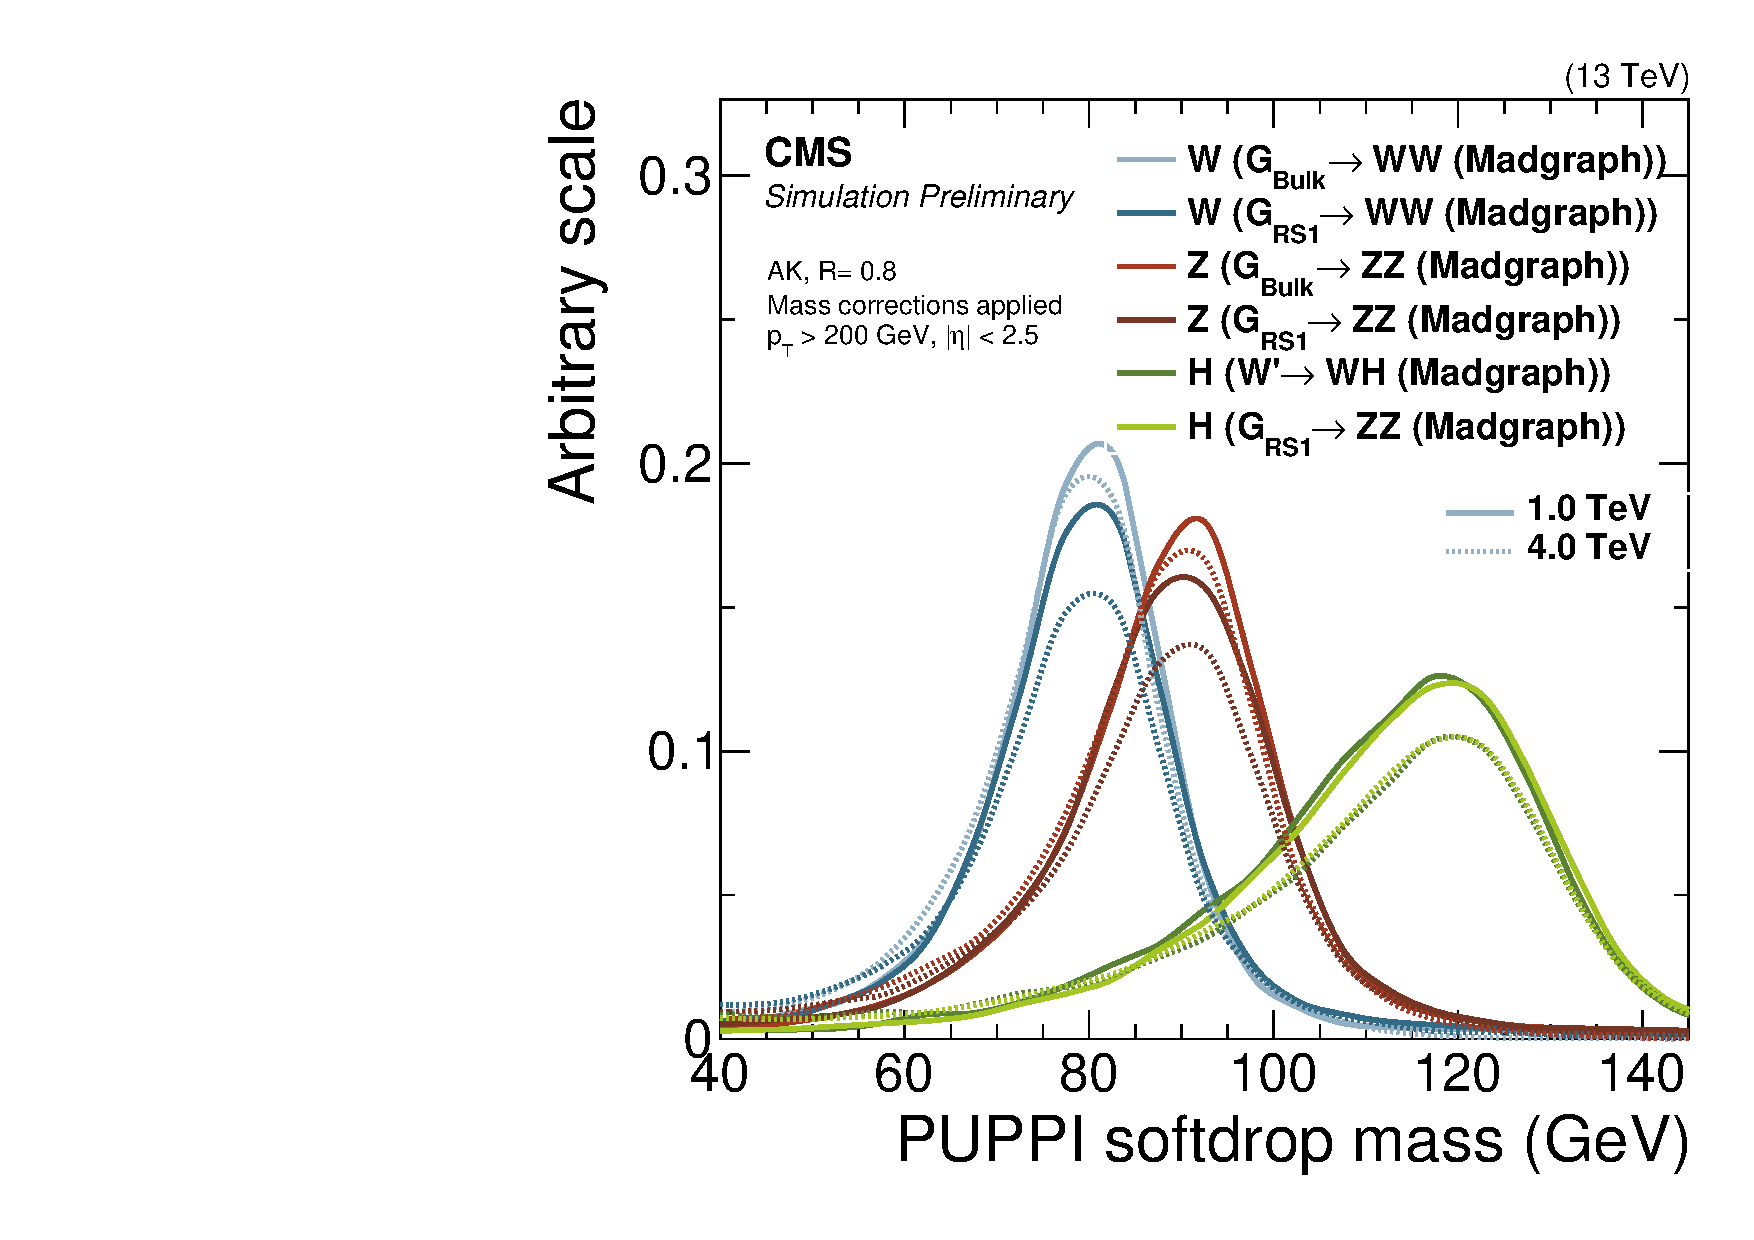
\includegraphics[width=0.49\textwidth]{figures/analysis/search2/AN-16-235/plots/SoftdropMass_NEWCORR_wH0.pdf}
\caption{The corrected PUPPI softdrop jet mass for W, Z, and H jets from different signal samples with masses of 1 and 4 TeV.}
\label{fig:search2:corrMass}
\end{figure}

\subsection{W-tagging performance}
\label{sec:searchII:vtagperf}
The new PUPPI softdrop based V tagger uses a softdrop jet mass window of $65 \GeV < m_{SD} < 105 \GeV$ in combination with a selection of PUPPI $\tau_{21}<0.4$.
We compare its performance to that of the CHS pruning-based tagger used in Search I as well as to that of a "DDT-transformed" \nsubj-based tagger~\cite{Dolen:2016kst}. The \ddt variable is a linear transformation of \nsubj given as
\begin{equation}
\label{eq:searchII:ddt}
\tau_{21}^{DDT} = \tau_{21} + M \times \log \bigg( \frac{m^2}{p_T \times 1 \textrm{ GeV}}\bigg)
\end{equation}
where $M=-0.063$ is obtained from a fit of $\tau_{21}$ against the variable $\rho^{'}=\log(m^2/\PT/\mu)$ in QCD Monte Carlo, where $\mu = 1 \GeV$.
The purpose of this is to decorrelate $\tau_{21}$ from the QCD jet softdrop mass and \PT, yielding a mass and dijet invariant mass spectrum minimally sculpted by a cut on the $\tau_{21}^{DDT}$ tagging variable. This tagger will be further explored, and described in detail, in the context of Search III in Section~\ref{sec:searchIII:ddt}.\par
The background rejection efficiency for QCD light-flavor jets as a function of W-jet signal efficiency is shown in Figure~\ref{fig:searchII:roc}.
The efficiency is measured after requiring a softdrop jet mass selection of $65 \GeV < m_{SD} < 105 \GeV$, while scanning the cut on \nsubj.
\begin{figure}[h!]
\centering
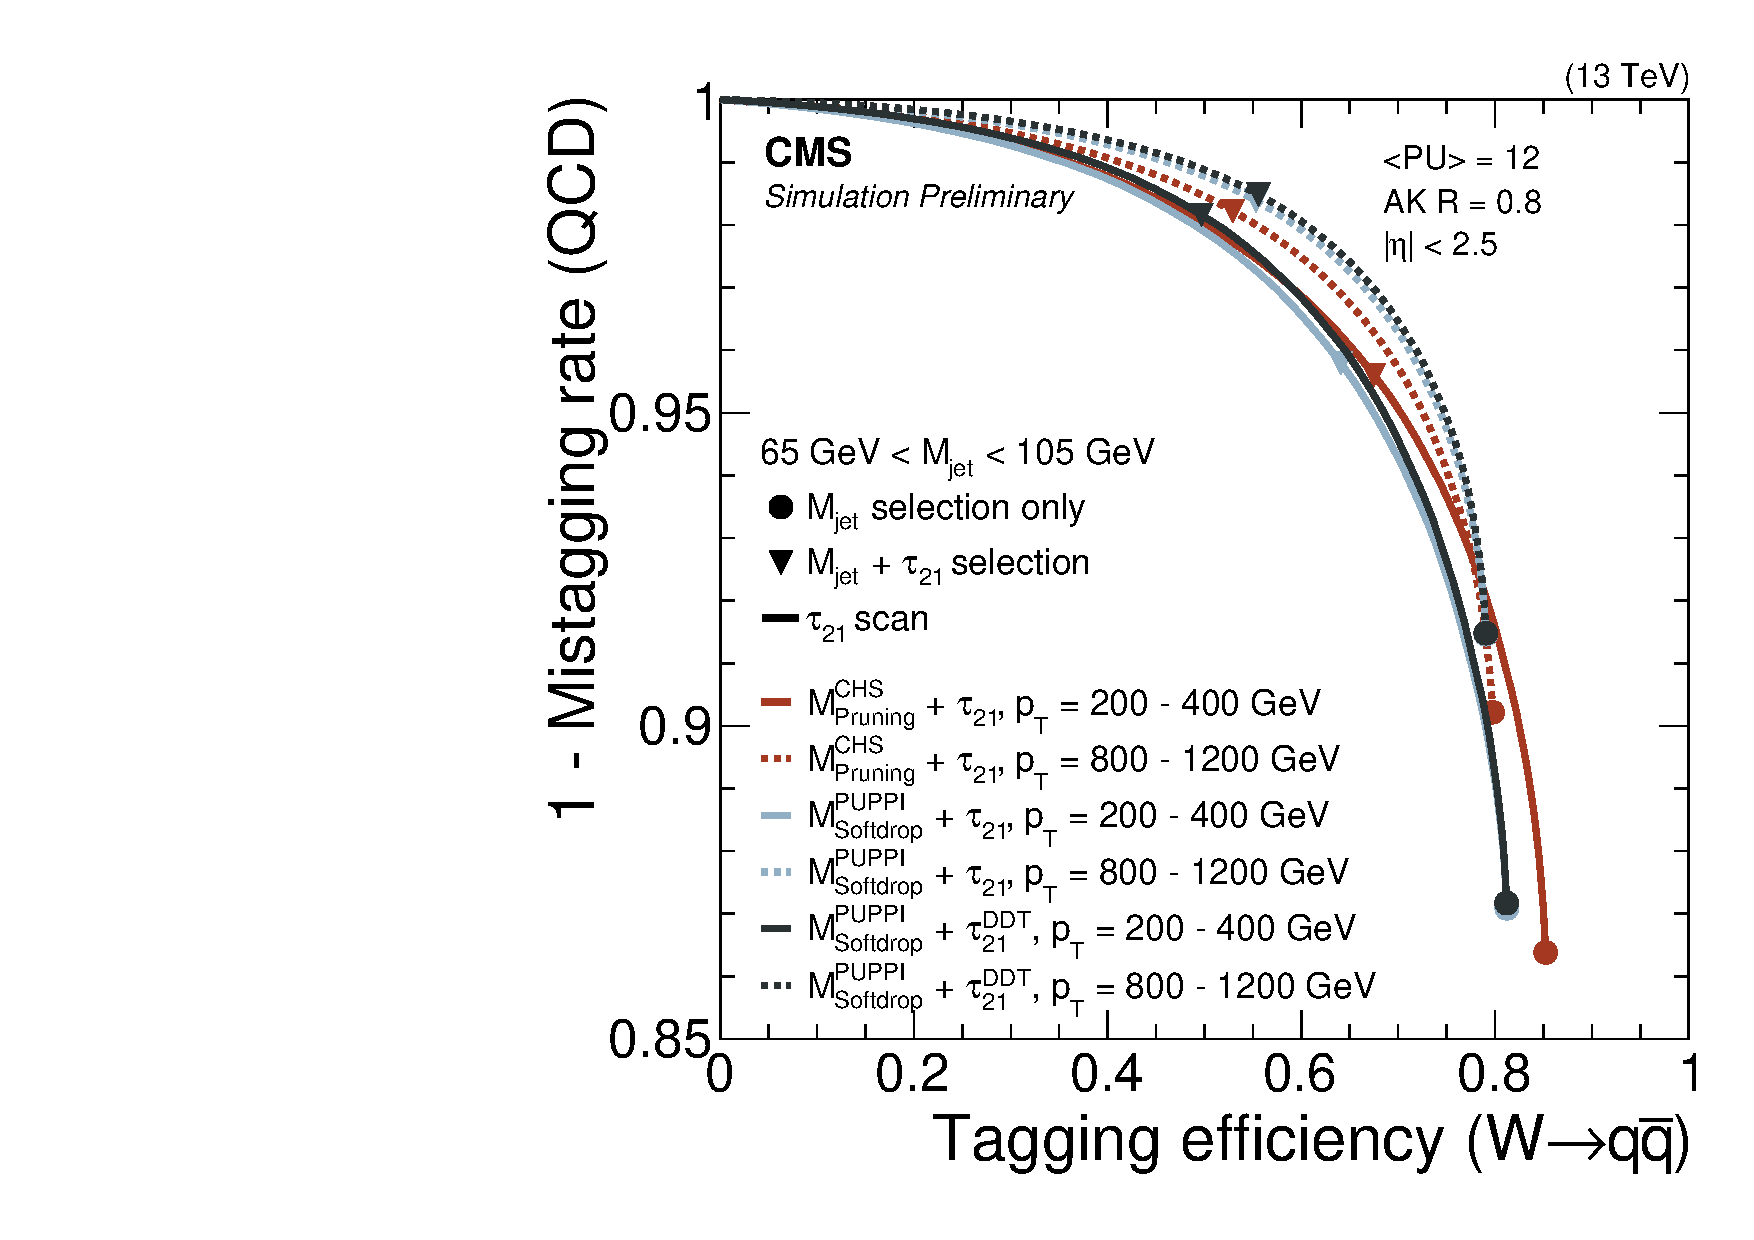
\includegraphics[width=0.49\textwidth]{figures/vtagging/JME-16-003/BoostedW/roc_WqqvsQCD_2bins.pdf}
\caption{The background rejection efficiency for QCD light-flavor jets as a function of W-jet signal efficiency. A cut on CHS pruned or PUPPI softdrop jet mass of $65<m_{\mathrm{p/sd}}<105$~\GeV is applied while scanning the cut on \nsubj. The cuts corresponding to $\tau_2/\tau_1 < 0.45$ for CHS pruned jets, PUPPI $\nsubj < 0.4$ or $\ddt<0.52$ for PUPPI softdrop jets are indicated with triangles, while the solid circles represent the efficiency and mistag rate for a mass cut only.}
\label{fig:searchII:roc}
\end{figure}
The general performance of each tagger is very similar, with the PUPPI softdrop-based taggers displaying a slightly higher signal efficiency for a given mistag rate at high \PT and CHS pruning-based taggers performing slightly better at low \PT.
In order to better understand the difference between each tagger, we look at the tagging performance as a function of jet \PT and pileup, as shown in Figure~\ref{fig:searchII:effvspt} and~\ref{fig:searchII:effvspu}. In Figure~\ref{fig:searchII:effvspt} we observe that the signal efficiency for a PUPPI softdrop or a CHS pruned jet mass selection is flat and around 80\% as a function of jet \PT. The QCD mistagging rate, on the other hand, falls of as a function of \PT, with a 1-3\% lower mistagging rate when using PUPPI softdrop jet mass than when using CHS pruned jet mass.
\begin{figure}[h!]
\centering
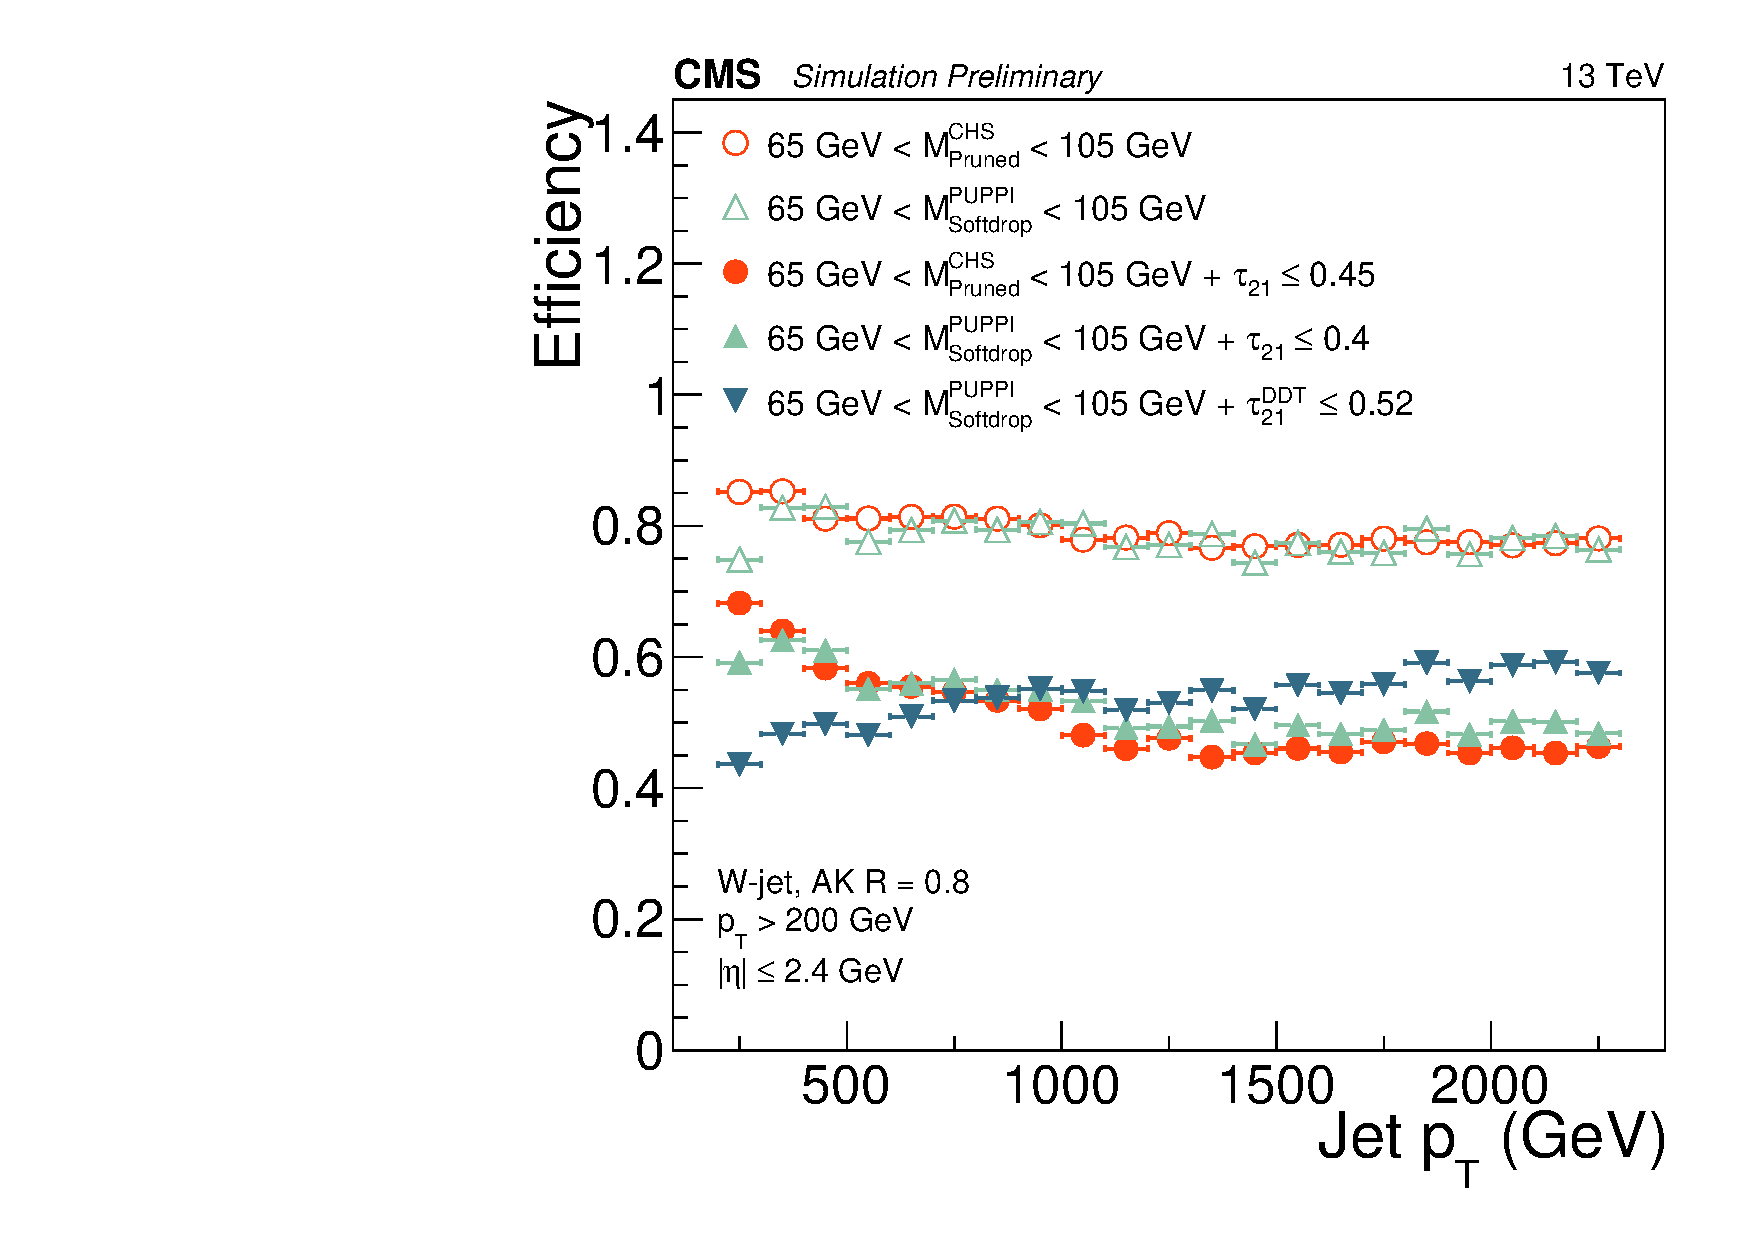
\includegraphics[width=0.49\textwidth]{figures/vtagging/JME-16-003/BoostedW/WtagSigEffvsPT.pdf}
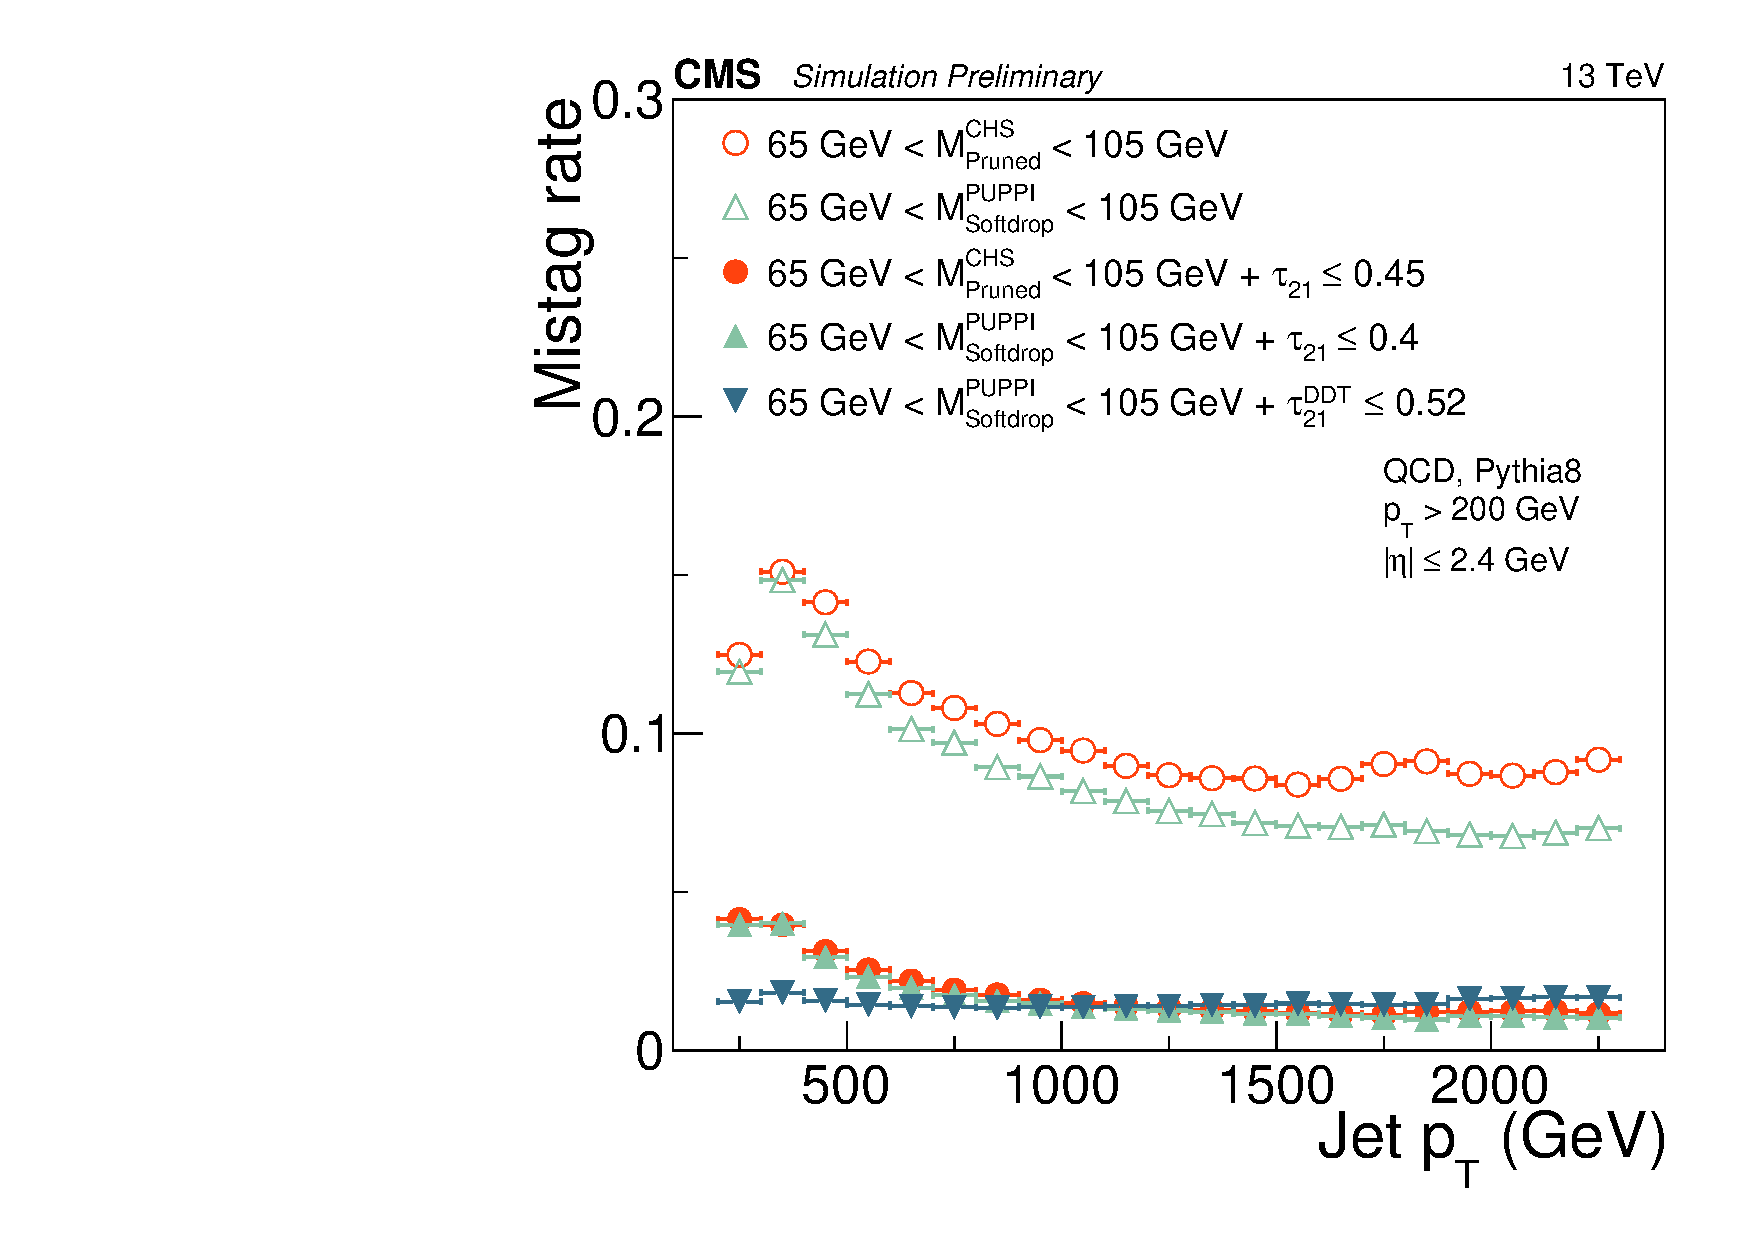
\includegraphics[width=0.49\textwidth]{figures/vtagging/JME-16-003/BoostedW/QCDBkgEffvsPT.pdf}
\caption{W-jet efficiency (left) and QCD light-flavor jet mistag rate (right) for a PUPPI softdrop or CHS pruned jet mass selection only (hollow circles) and the combined $m_{\mathrm{p/sd}}$ + (PUPPI) \nsubj (DDT) selection (solid circles) as a function of jet \PT.}
\label{fig:searchII:effvspt}
\end{figure}
Once applying an n-subjettiness cut, the signal efficiency as well as the mistag rate for the \nsubj-based taggers becomes smaller as a function of jet \PT, with an average signal efficiency of around 50\% for a $\sim 2\%$ mistag rate. An interesting behavior is observed for the \ddt tagger: while the mistagging rate is flat as a function of \PT, by construction, the signal efficiency gets higher as the \PT increases, outperforming the other taggers above 1 \TeV. \par
Figure~\ref{fig:searchII:effvspu} shows the W-jet tagging efficiency (left) and QCD light-flavor jet mistagging rate (right) as a function of the number of interaction vertices in the event. The tagging efficiency of the CHS pruned jet tagger (red solid circles) falls off steeply versus the number of primary vertices in the event, while the PUPPI softdrop taggers (light and dark blue solid circles) are more or less insensitive to pileup.
\begin{figure}[h!]
\centering
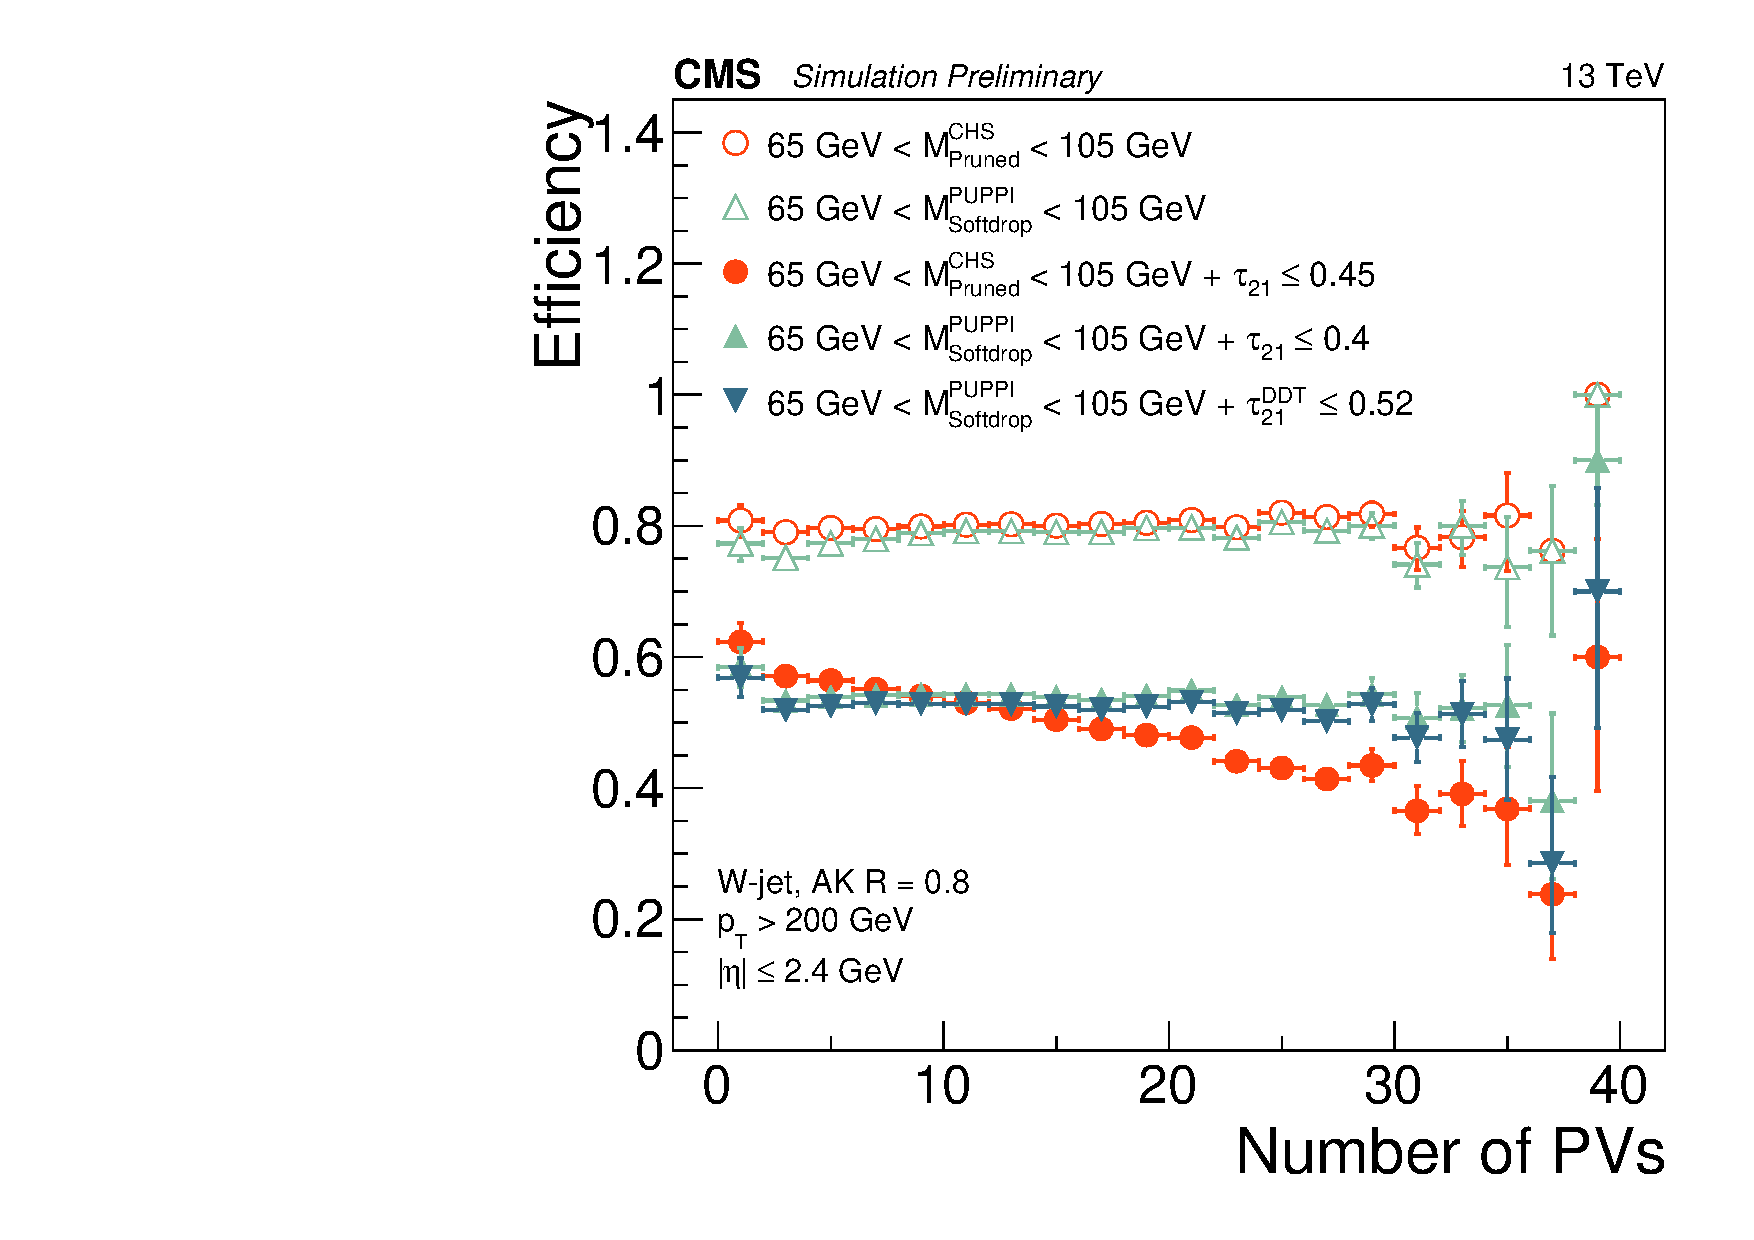
\includegraphics[width=0.49\textwidth]{figures/vtagging/JME-16-003/BoostedW/WtagSigEffvsNPV.pdf}
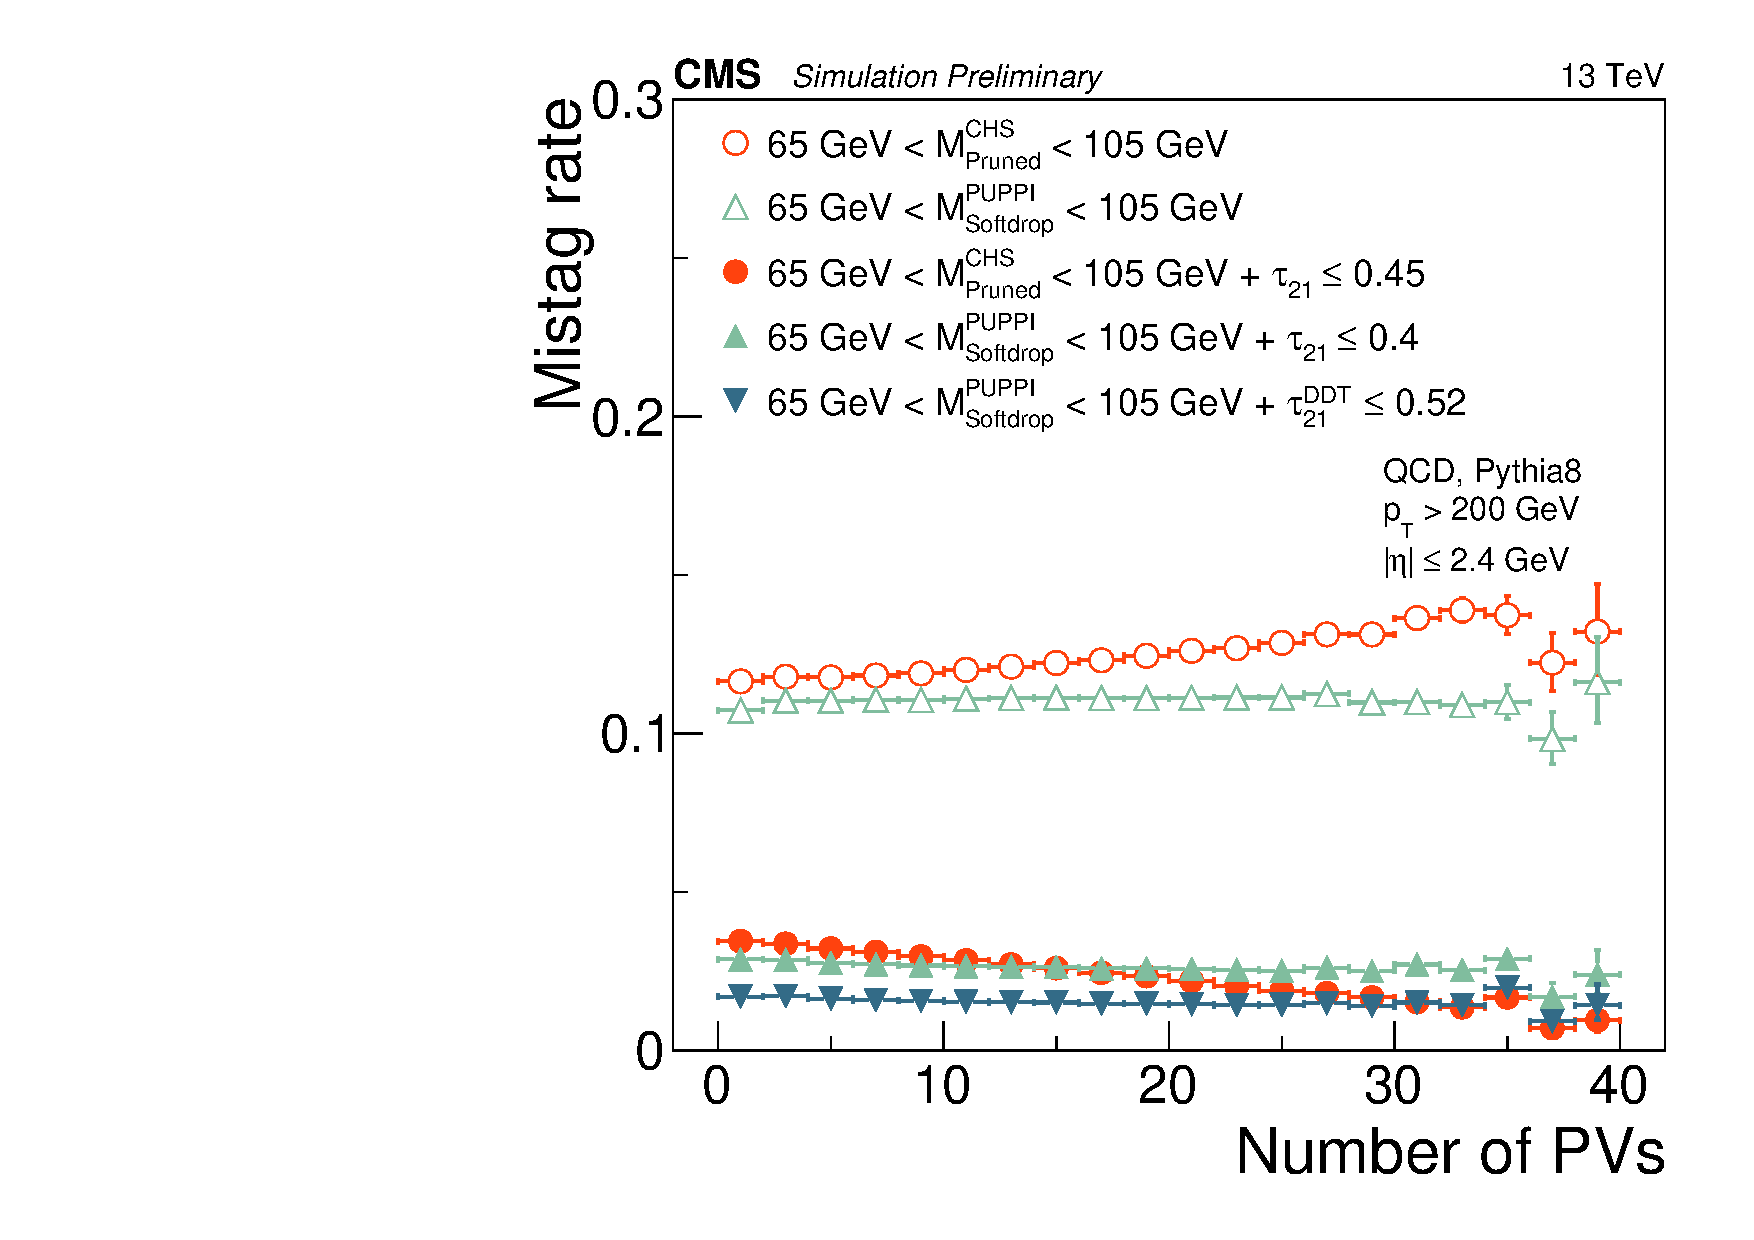
\includegraphics[width=0.49\textwidth]{figures/vtagging/JME-16-003/BoostedW/QCDBkgEffvsNPV.pdf}
\caption{W-jet efficiency (left) and QCD light-flavor jet mistag rate (right) for a PUPPI softdrop or CHS pruned jet mass selection only (hollow circles) and the combined $m_{\mathrm{p/sd}}$ + (PUPPI) \nsubj (DDT) selection (solid circles) as a function of the number of interaction vertices in the event.}
\label{fig:searchII:effvspu}
\end{figure}
The per-jet efficiency of the PUPPI softdrop and PUPPI \nsubj tagger is around 50-55\% for a 1-2\% mistag rate. Based on the observed general performance, tagging stability versus pileup, and due to theoretical considerations, PUPPI softdrop jet mass with dedicated mass corrections applied, together with PUPPI \nsubj, is chosen as the W tagger for this analysis.

\subsection{Efficiency scale factors, jet mass scale and resolution} 
\label{sec:searchII:wtagsf}
In order to measure the W-tagging efficiency, and jet-mass scale and resolution for the new PUPPI softdrop jet mass tagger, we use the same procedure as outlined in Section~\ref{sec:searchI:vtag}. The first commissioning of the new tagger was done using 2.3 \fbinv of data collected in 2015, and was published in a jet algorithms performance note~\cite{CMS-PAS-JME-16-003}. The measurements were then redone using 12.9 and 35.9 \fbinv of data collected in 2016 for the two analyses presented in this chapter (the latter measurement was performed by a separate analysis team). The results shown in the following will be those obtained when the V tagger was first presented in an analysis context, corresponding to the PAS based on 12.9 \fbinv of data collected in the beginning of 2016. Since the fit method is outlined in detail in Section~\ref{sec:searchI:vtag}, fits to matched \ttbar MC and minor backgrounds for the PUPPI softdrop based tagger are skipped here and can be found in Appendix~\ref{app:sf16}.\par
%In order to better understand the differences between the CHS pruning and PUPPI+softdrop based taggers, the first efficiency measurement was done in parallel for both algorithms, requiring either a softdrop or a pruned jet mass between 40 \GeV and 150 \GeV. 
%The softdrop jet mass is computed after PUPPI and the jet mass corrections as described in Section~\ref{sec:searchII:masscorr} are applied, while the pruned mass is corrected with L2L3 jet energy corrections. 
The PUPPI softdrop jet mass and the PUPPI $\tau_{21}$ variable in data and MC are shown in Figure~\ref{fig:searchII:ttbarcp}. These can be compared to the corresponding plots for the CHS pruned jet mass and \nsubj distributions in Figure~\ref{fig:searchII:ttbarcp}. The softdrop and pruned jet mass distributions, as well as the PUPPI and CHS \nsubj variables, are very similar and the variables are described equally well in simulation.
\begin{figure}[h!]
\centering
\begin{tabular}{cc}
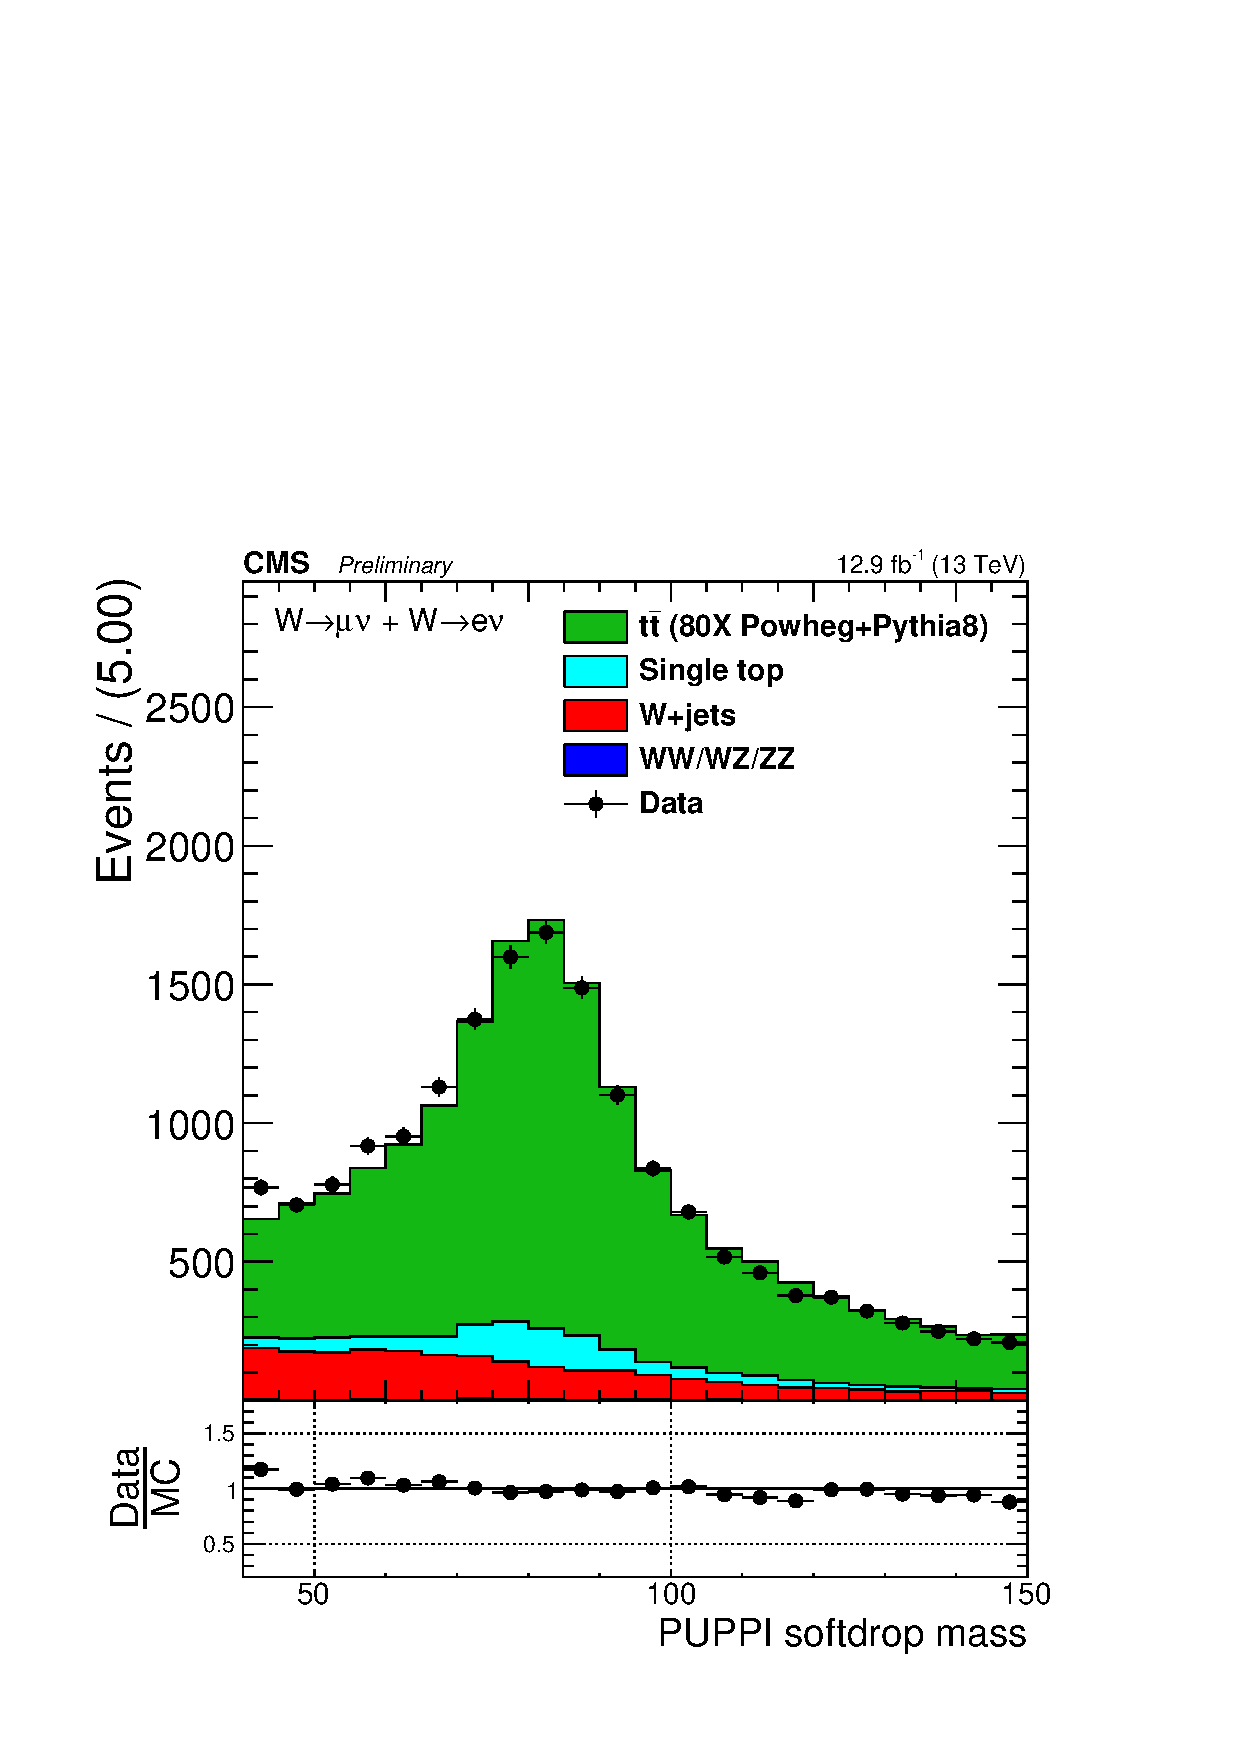
\includegraphics[width=0.5\textwidth]{figures/vtagging/AN-16-342/controlplots/Whadr_puppi_softdrop_powheg.pdf}
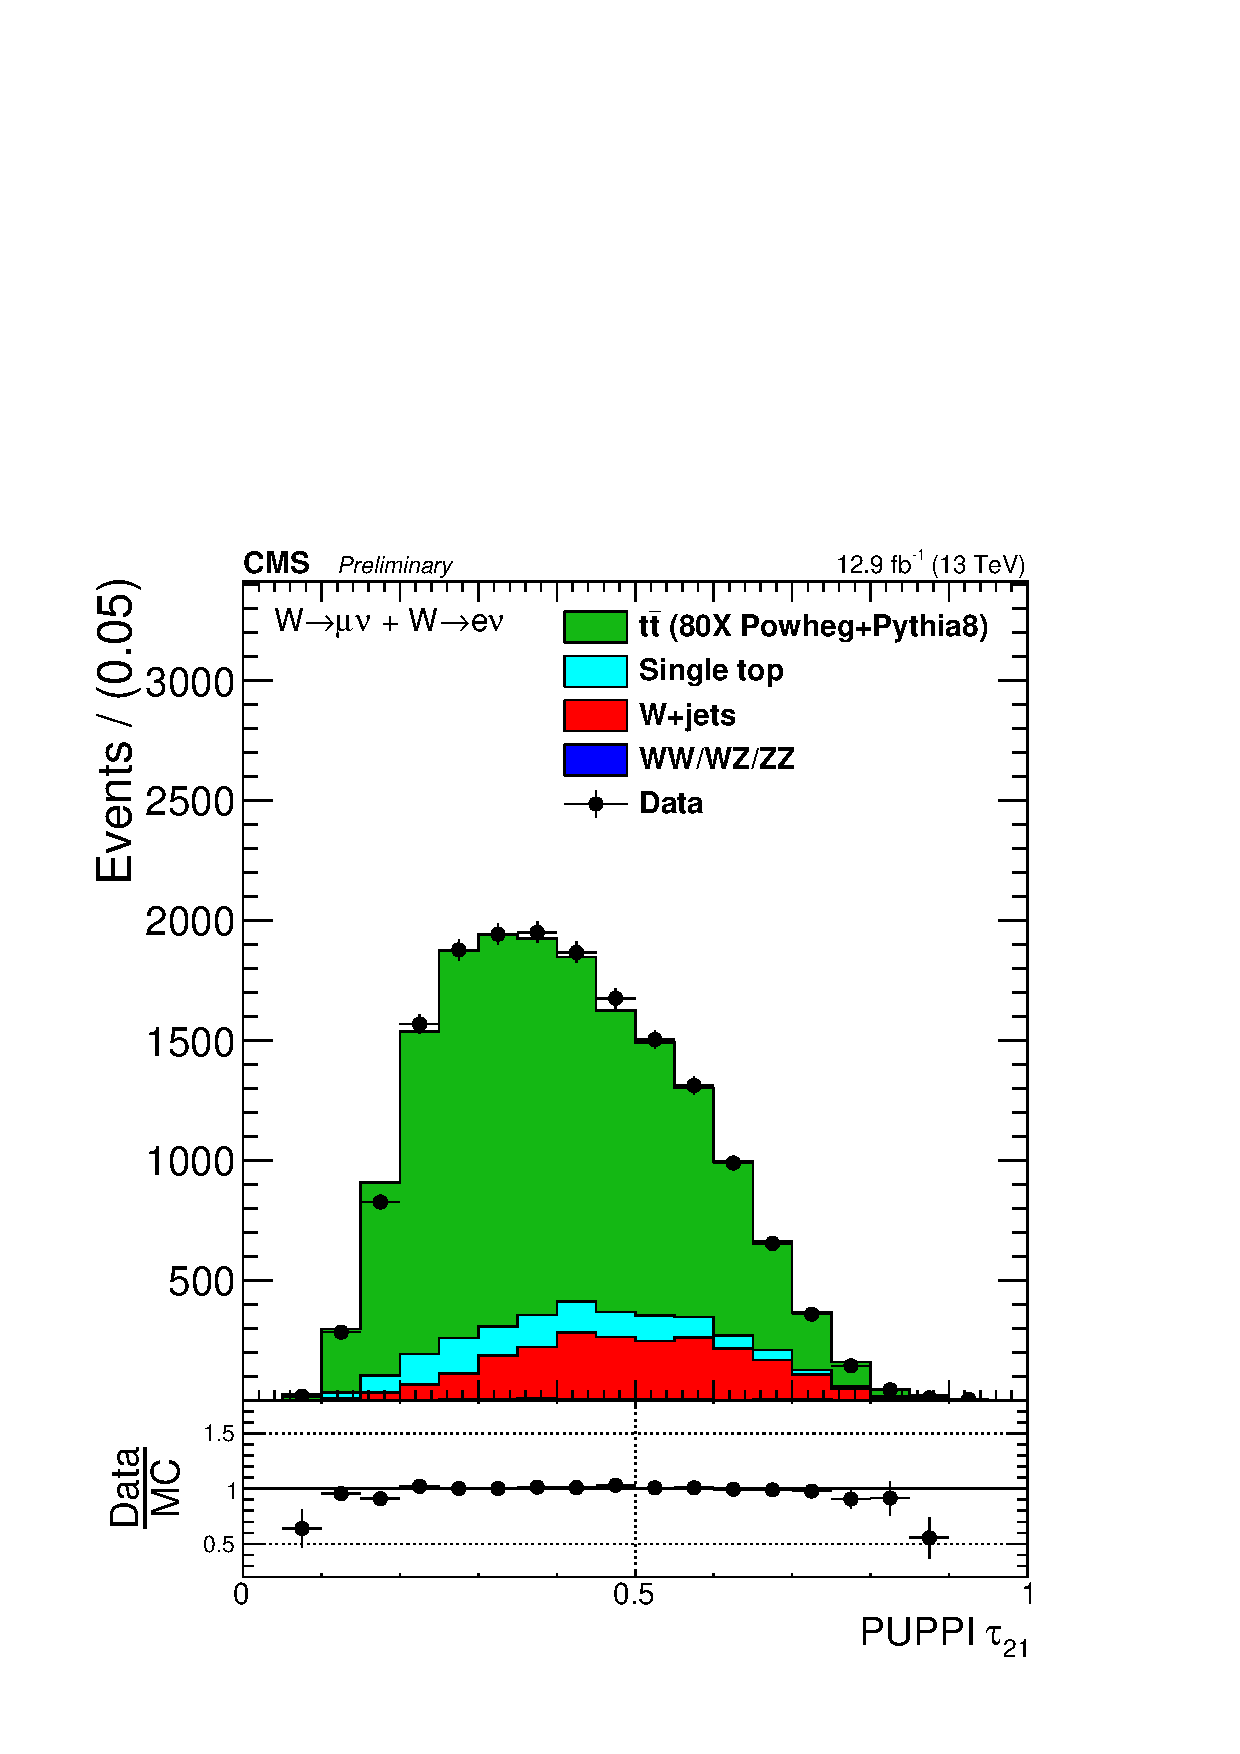
\includegraphics[width=0.5\textwidth]{figures/vtagging/AN-16-342/controlplots/Whadr_puppi_tau2tau1_powheg.pdf}\\
\end{tabular}
\caption{Distribution of the PUPPI softdrop mass (left) and PUPPI n-subjettiness (right) distribution in the \ttbar control sample.}
\label{fig:searchII:ttbarcp}
\end{figure}
Following what was done in Section~\ref{sec:searchI:vtag}, we extract and compare the W-tagging efficiency, jet mass scale and jet mass resolution of the combined jet mass and \nsubj selection in data and in MC. This is done through a simultaneous fit of the the softdrop jet mass spectrum between 40 and 150 \GeV in two regions:
\begin{itemize}
\itemsep0em
  \item pass region: $0 <  \nsubj \leq 0.40$ $\sim$ high purity, and
  \item fail region: $0.40 < \nsubj \leq 0.75$ $\sim$ low purity.
\end{itemize}
The fits are shown in Figure~\ref{fig:searchII:simfit}, with the corresponding extracted efficiencies from the Gaussian component of the total fit and scale factors summarized in Table~\ref{tab:searchII:WtagSFs}.
The quoted systematic uncertainties are evaluated in the same way as was described in Section~\ref{sec:searchI:wtagsystematic}, and correspond to the uncertainty due to the choice of ME generator and due to the choice of fit method.
\begin{table}[h!]
   \centering
   \footnotesize
   \begin{tabular}{l|l|c|c|c}
    & Working point & Eff. data & Eff. simulation & Scale factor\\
   \hline
   HP& $\nsubj < 0.4$         &  $0.839 \pm 0.020 $& $0.817 \pm 0.012$ &\SFWTAGHPWPT\\
   LP& $0.4 < \nsubj < 0.75$ &  $0.154 \pm 0.020 $& $0.176 \pm 0.012$ &\SFWTAGLPWPT\\
   \hline
   \end{tabular}
   \caption{W-tagging scale factors for both categories the high purity and low purity categories for two taggers: Pruned jet mass + \nsubj and PUPPI softdrop jet mass + PUPPI \nsubj. }
   \label{tab:searchII:WtagSFs}
\end{table}
\begin{figure}[h!]
\centering
% \includegraphics[width=0.44\textwidth]{figures/analysis/search2/AN-16-235/plots/TotalFit__HP0v40powheg_PuppiSD.pdf}      %12.9 fbinv
% \includegraphics[width=0.44\textwidth]{figures/analysis/search2/AN-16-235/plots/TotalFit__HP0v40powheg_PuppiSD_fail.pdf} %12.9 fbinv
\includegraphics[width=0.44\textwidth]{figures/vtagging/AN-16-342/TotalFit__HP0v40powheg_PuppiSD.pdf}
\includegraphics[width=0.44\textwidth]{figures/vtagging/AN-16-342/TotalFit__HP0v40powheg_PuppiSD_fail.pdf}\\
\caption{PUPPI softdrop jet mass distribution that pass (left) and fail (right) the PUPPI $\nsubj< 0.40$ selection. Results of both the fit to data (blue) and simulation (red) are shown and the background components of the fit are shown as short-dashed lines.}
\label{fig:searchII:simfit}
\end{figure}
Both scale factors are compatible with unity within uncertainties. We additionally extract the jet-mass scale and jet-mass resolution from the mean and width of the Gaussian component of the total fit in the pass region. These are summarized in Table~\ref{tab:searchII:wtagparams}. We find that the W-jet mass scale for PUPPI softdrop jet mass is identical in simulation and in data, whereas for pruning (Table~\ref{tab:searchI:params}) the difference was around 2\%, 
The jet mass resolution, on the other hand, is larger in data for PUPPI softdrop jet mass, by roughly 8\%, whereas for pruning the resolution is larger in simulation (11\%). However, both are statistically insignificant and compatible with unity within uncertainties.
\begin{table}[!h]
 \begin{center}
 \footnotesize
 \begin{tabular}{c|c|c|c}
  Parameter & Data & Simulation & Data/Simulation \\
  \hline
  PUPPI softdrop $\langle m \rangle$ & \WMASSDATAWPT~\GeV & \WMASSMCWPT~\GeV  &\JMS \\%New mass corrections
  PUPPI softdrop $\sigma$            & \WRESDATAWPT~\GeV  & \WRESMCWPT~\GeV   & \JMR \\%New mass corrections
  \hline
 \end{tabular}
 \caption{Summary of the fitted W-jet mass peak parameters.}
 \label{tab:searchII:wtagparams}
 \end{center}
\end{table}
The W-tagging efficiency scale factors, jet-mass and resolution scales affect the signal yield and are included in the analysis in the same way as was described in Section~\ref{sec:searchI:wtagimpact}, by scaling the total signal yield and incorporating an uncertainty on the signal efficiency due to a shift and broadening of the W-jet mass peak.

\subsection{W-tagging mistag rate measurement} 
\label{sec:searchII:wmistag}
The W-tagging light-flavor jet mistagging rate is measured in a QCD dijet-enriched region in data and is compared to the prediction from QCD MC using three different combinations of generators: \HERWIG{++}, \PYTHIA{8}, and \MADGRAPH{}+\PYTHIA{8}.
Figure~\ref{fig:searchII:fakerate} shows the mistagging rate as a function of jet \PT for three different taggers: CHS pruning and \nsubj, PUPPI softdrop and \nsubj, and PUPPI softdrop and \ddt.
\begin{figure}[h!]
\centering
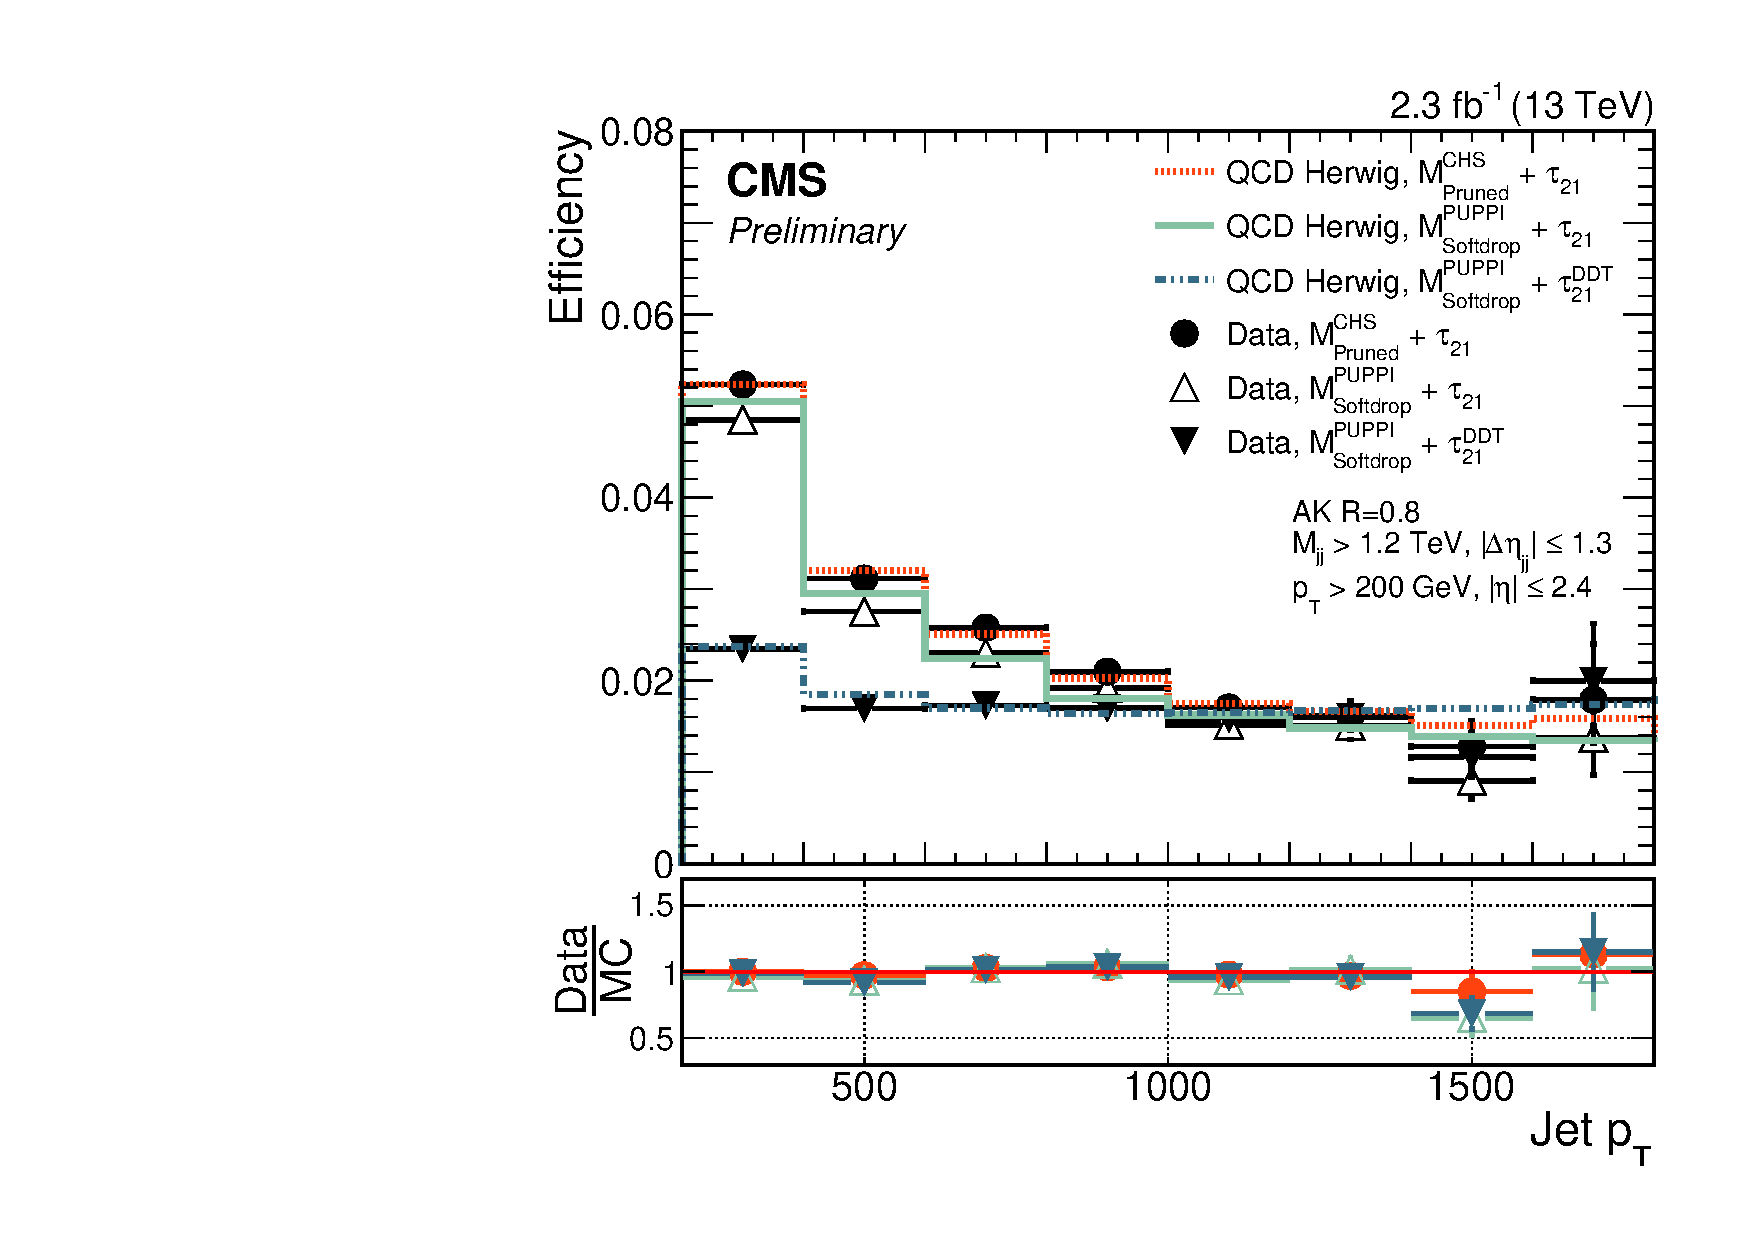
\includegraphics[width=0.49\textwidth]{figures/vtagging/JME-16-003/BoostedW/BkgEff_DataMC_herwig_pT.pdf}
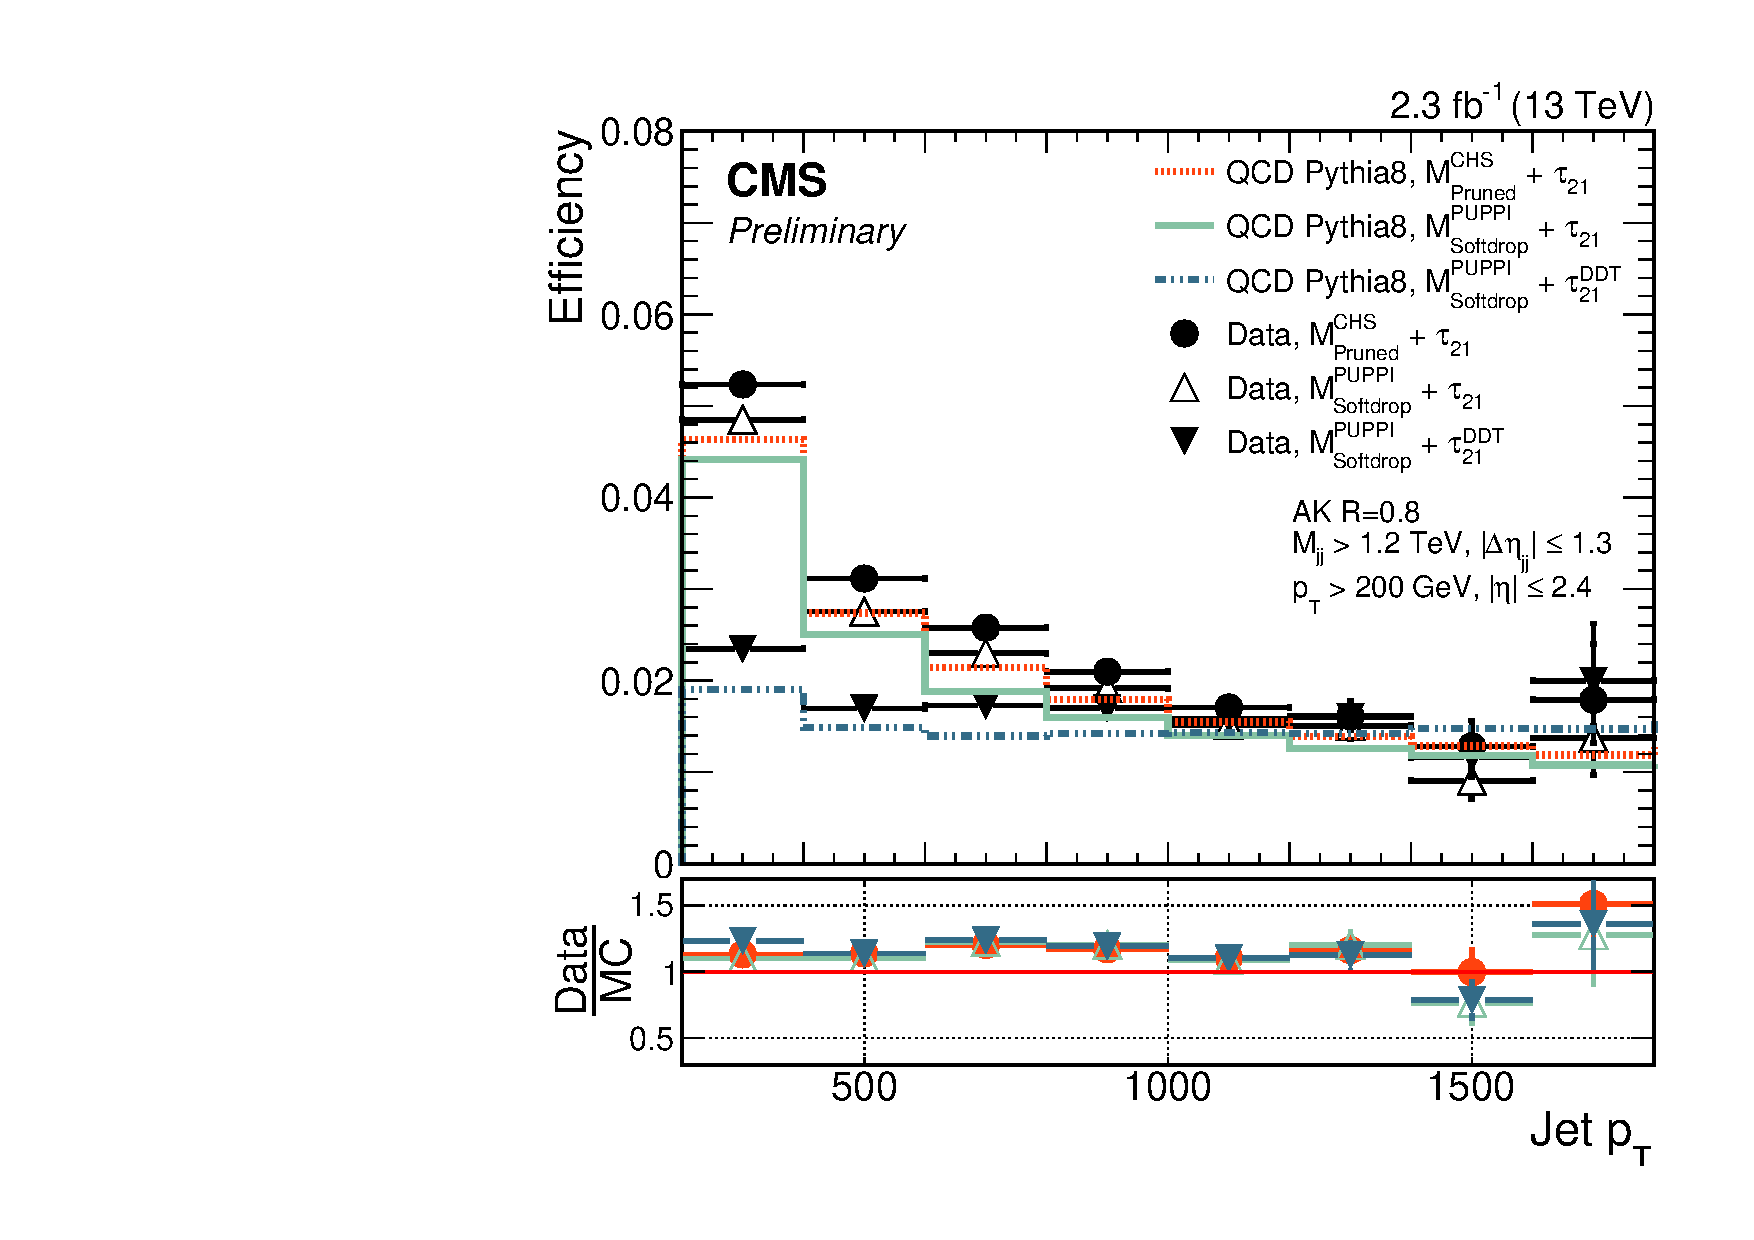
\includegraphics[width=0.49\textwidth]{figures/vtagging/JME-16-003/BoostedW/BkgEff_DataMC_Pythia8_pT.pdf}\\
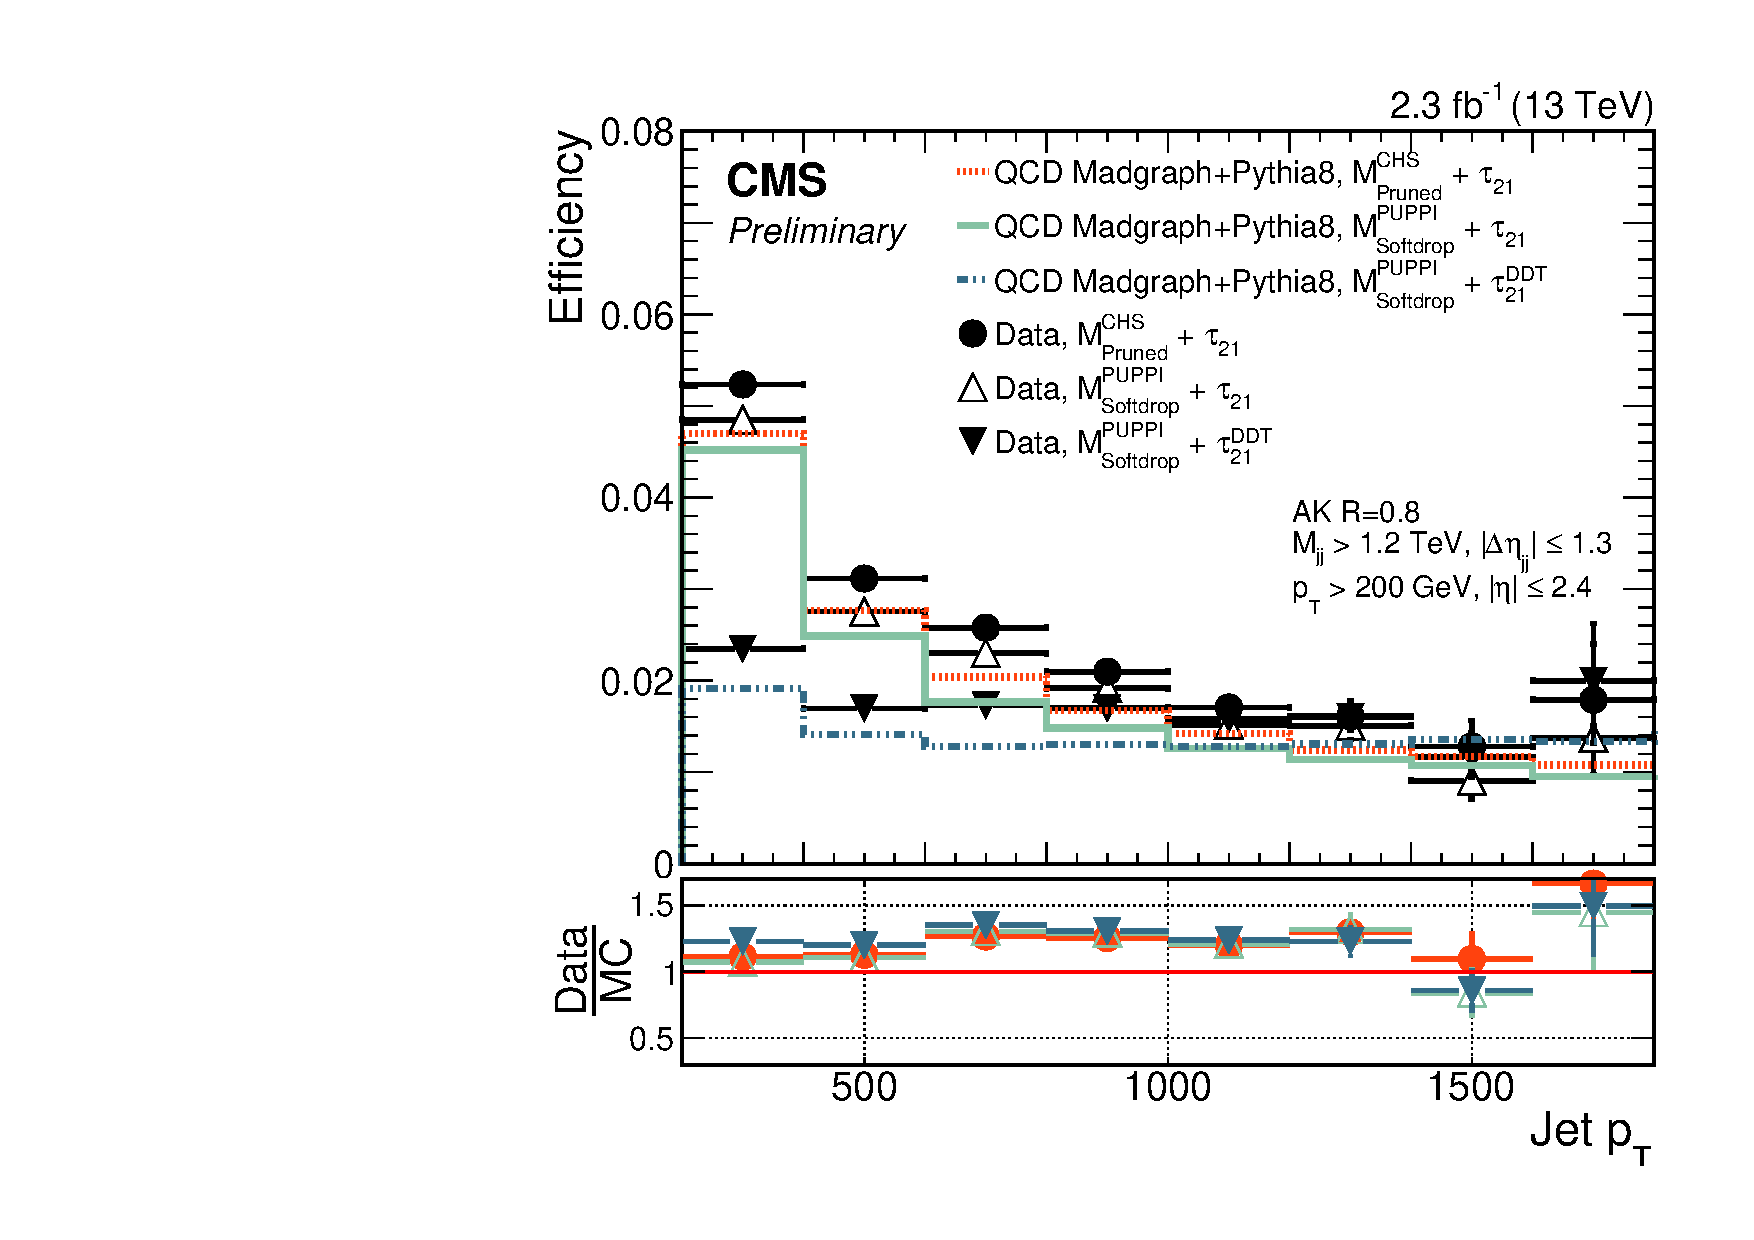
\includegraphics[width=0.49\textwidth]{figures/vtagging/JME-16-003/BoostedW/BkgEff_DataMC_Pythia8Madgraph_pT.pdf}
\caption{ 
The fraction of jets that pass the $m_{\mathrm{p/sd}}$ and \nsubj selections in a dijet enriched sample for data and for simulation as a function of jet \PT. Here the comparison is between \HERWIG{++} (top left), \PYTHIA{8} (top right), and \PYTHIA{8} with \MADGRAPH as the matrix-element generator (bottom).}
\label{fig:searchII:fakerate}
\end{figure}
We find a substantial difference in the modeling of substructure variables between the different generators, most likely coming from their very different description of gluon radiation (dominant in QCD multijet events).
The best description is obtained with \HERWIG{++}, while all three generators model the \PT-dependence of the tagger well.\par
We additionally study how a selection on \nsubj and \ddt affect the total quark and gluon content of the QCD background. Figure~\ref{fig:searchII:qgfakerate} shows the stacked relative quark and gluon content in a \PYTHIA{8} QCD dijet sample for selection requirements based on PUPPI \nsubj and \ddt. We see that the quark content increases as a function of jet \PT when applying a selection on \ddt, while it decreases when applying a selection on \nsubj.
\begin{figure}[h!]
\centering
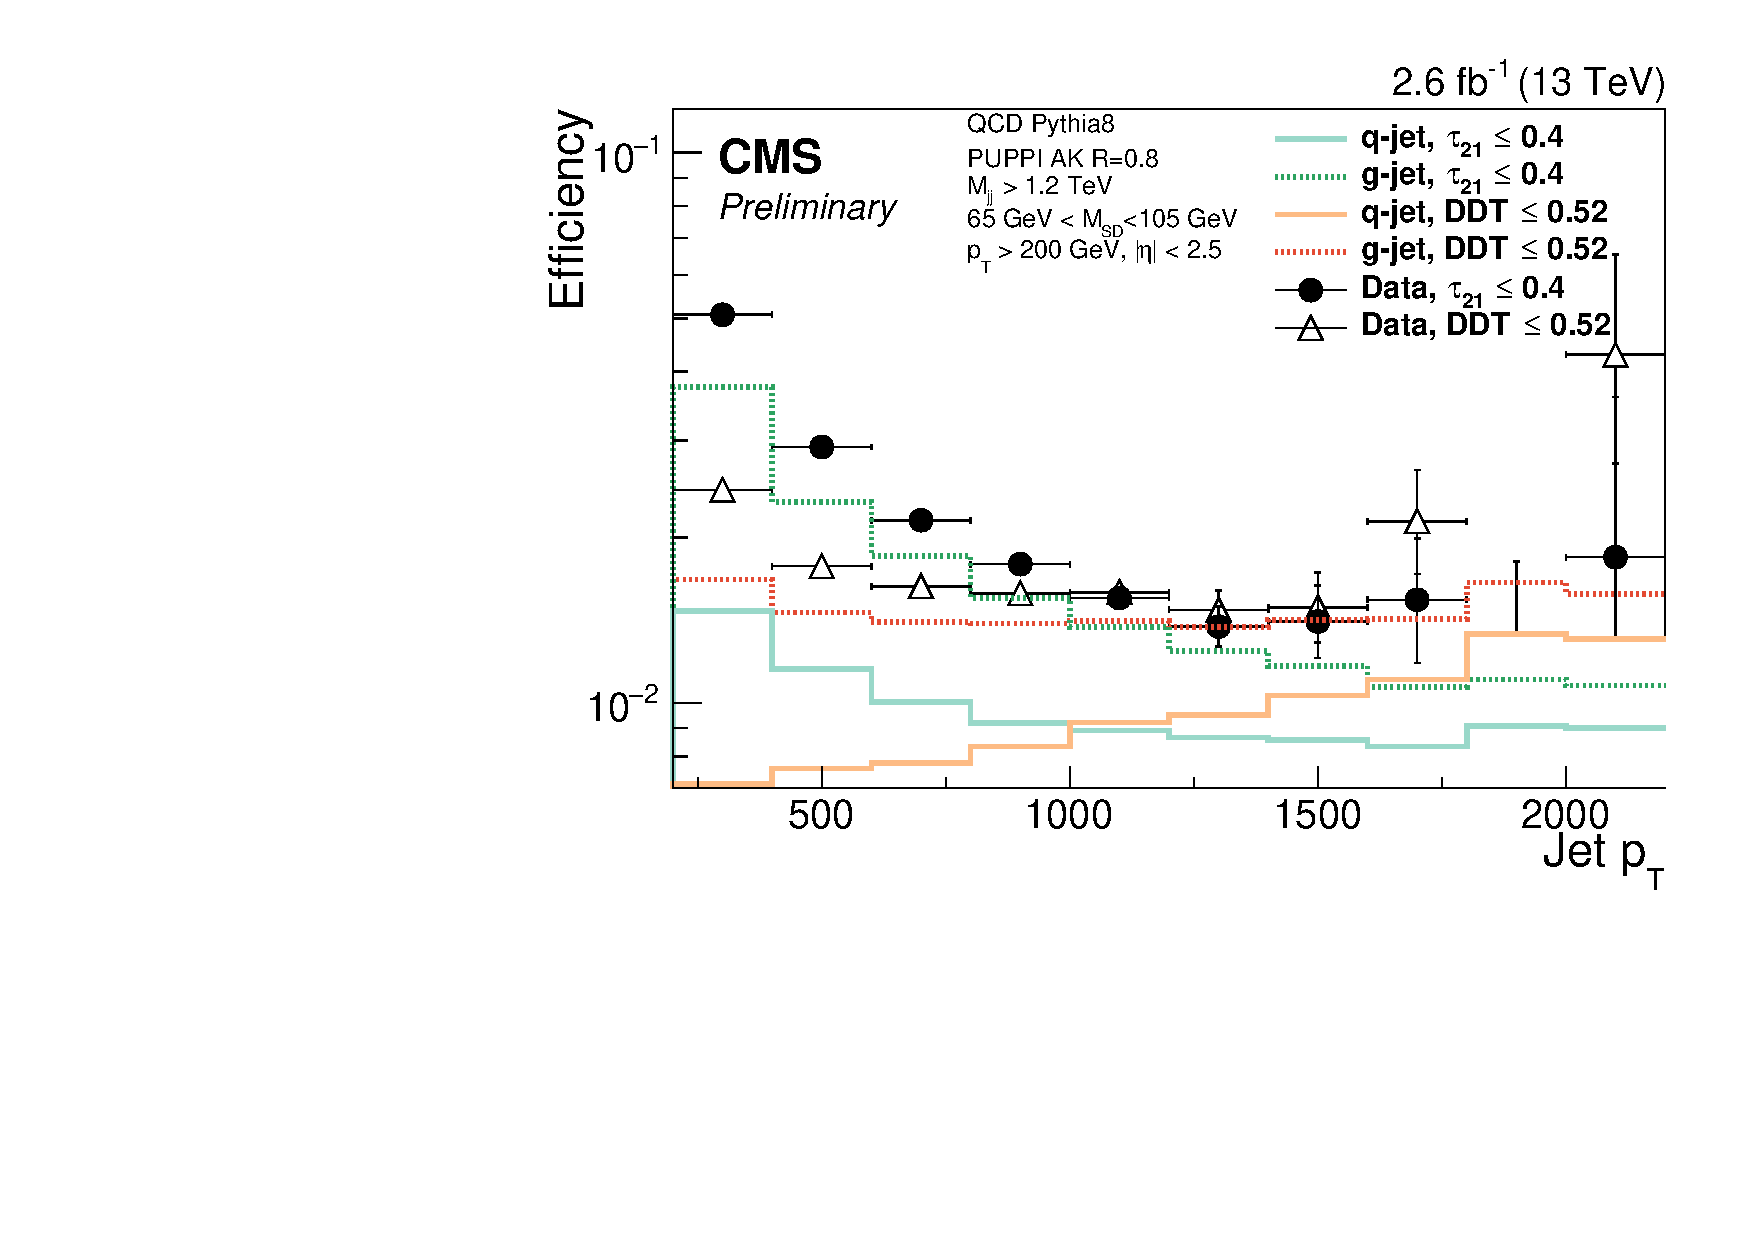
\includegraphics[width=0.49\textwidth]{figures/vtagging/JME-16-003/BoostedW/qgFakeRate_Pythia8_pT.pdf}
\caption{ 
The fraction of jets that pass the PUPPI softdrop jet mass selection and a selection on \nsubj (turquoise) or \ddt (orange) in a dijet-enriched sample. The jets from QCD MC are split into two contributions: jets originating from gluons (dotted line) and jets originating from quarks (solid line).}
\label{fig:searchII:qgfakerate}
\end{figure}
 This can be attributed to the fact that the distribution of jet mass divided by the jet \PT, $m/\PT$, for quark and gluon jets are very different from one another, and these differences increase as the jet \PT increases. Figure~\ref{fig:searchII:mpt_qvsg} shows the mass divided by \PT for jets originating from a quark (blue) or a gluon (red), for jets with a \PT of 200 \GeV (left) or 1600 \GeV (right). We see that the jet mass divided by the jet \PT peaks at significantly higher values for gluon jets than for quark jets. From the definition of the \ddt tagger in Equation~\ref{eq:searchII:ddt}, it can therefore be seen that a selection on \ddt will act more aggressively on jets with a high $m/\PT$, effectively removing more gluon jets.
\begin{figure}[ht!]
\centering
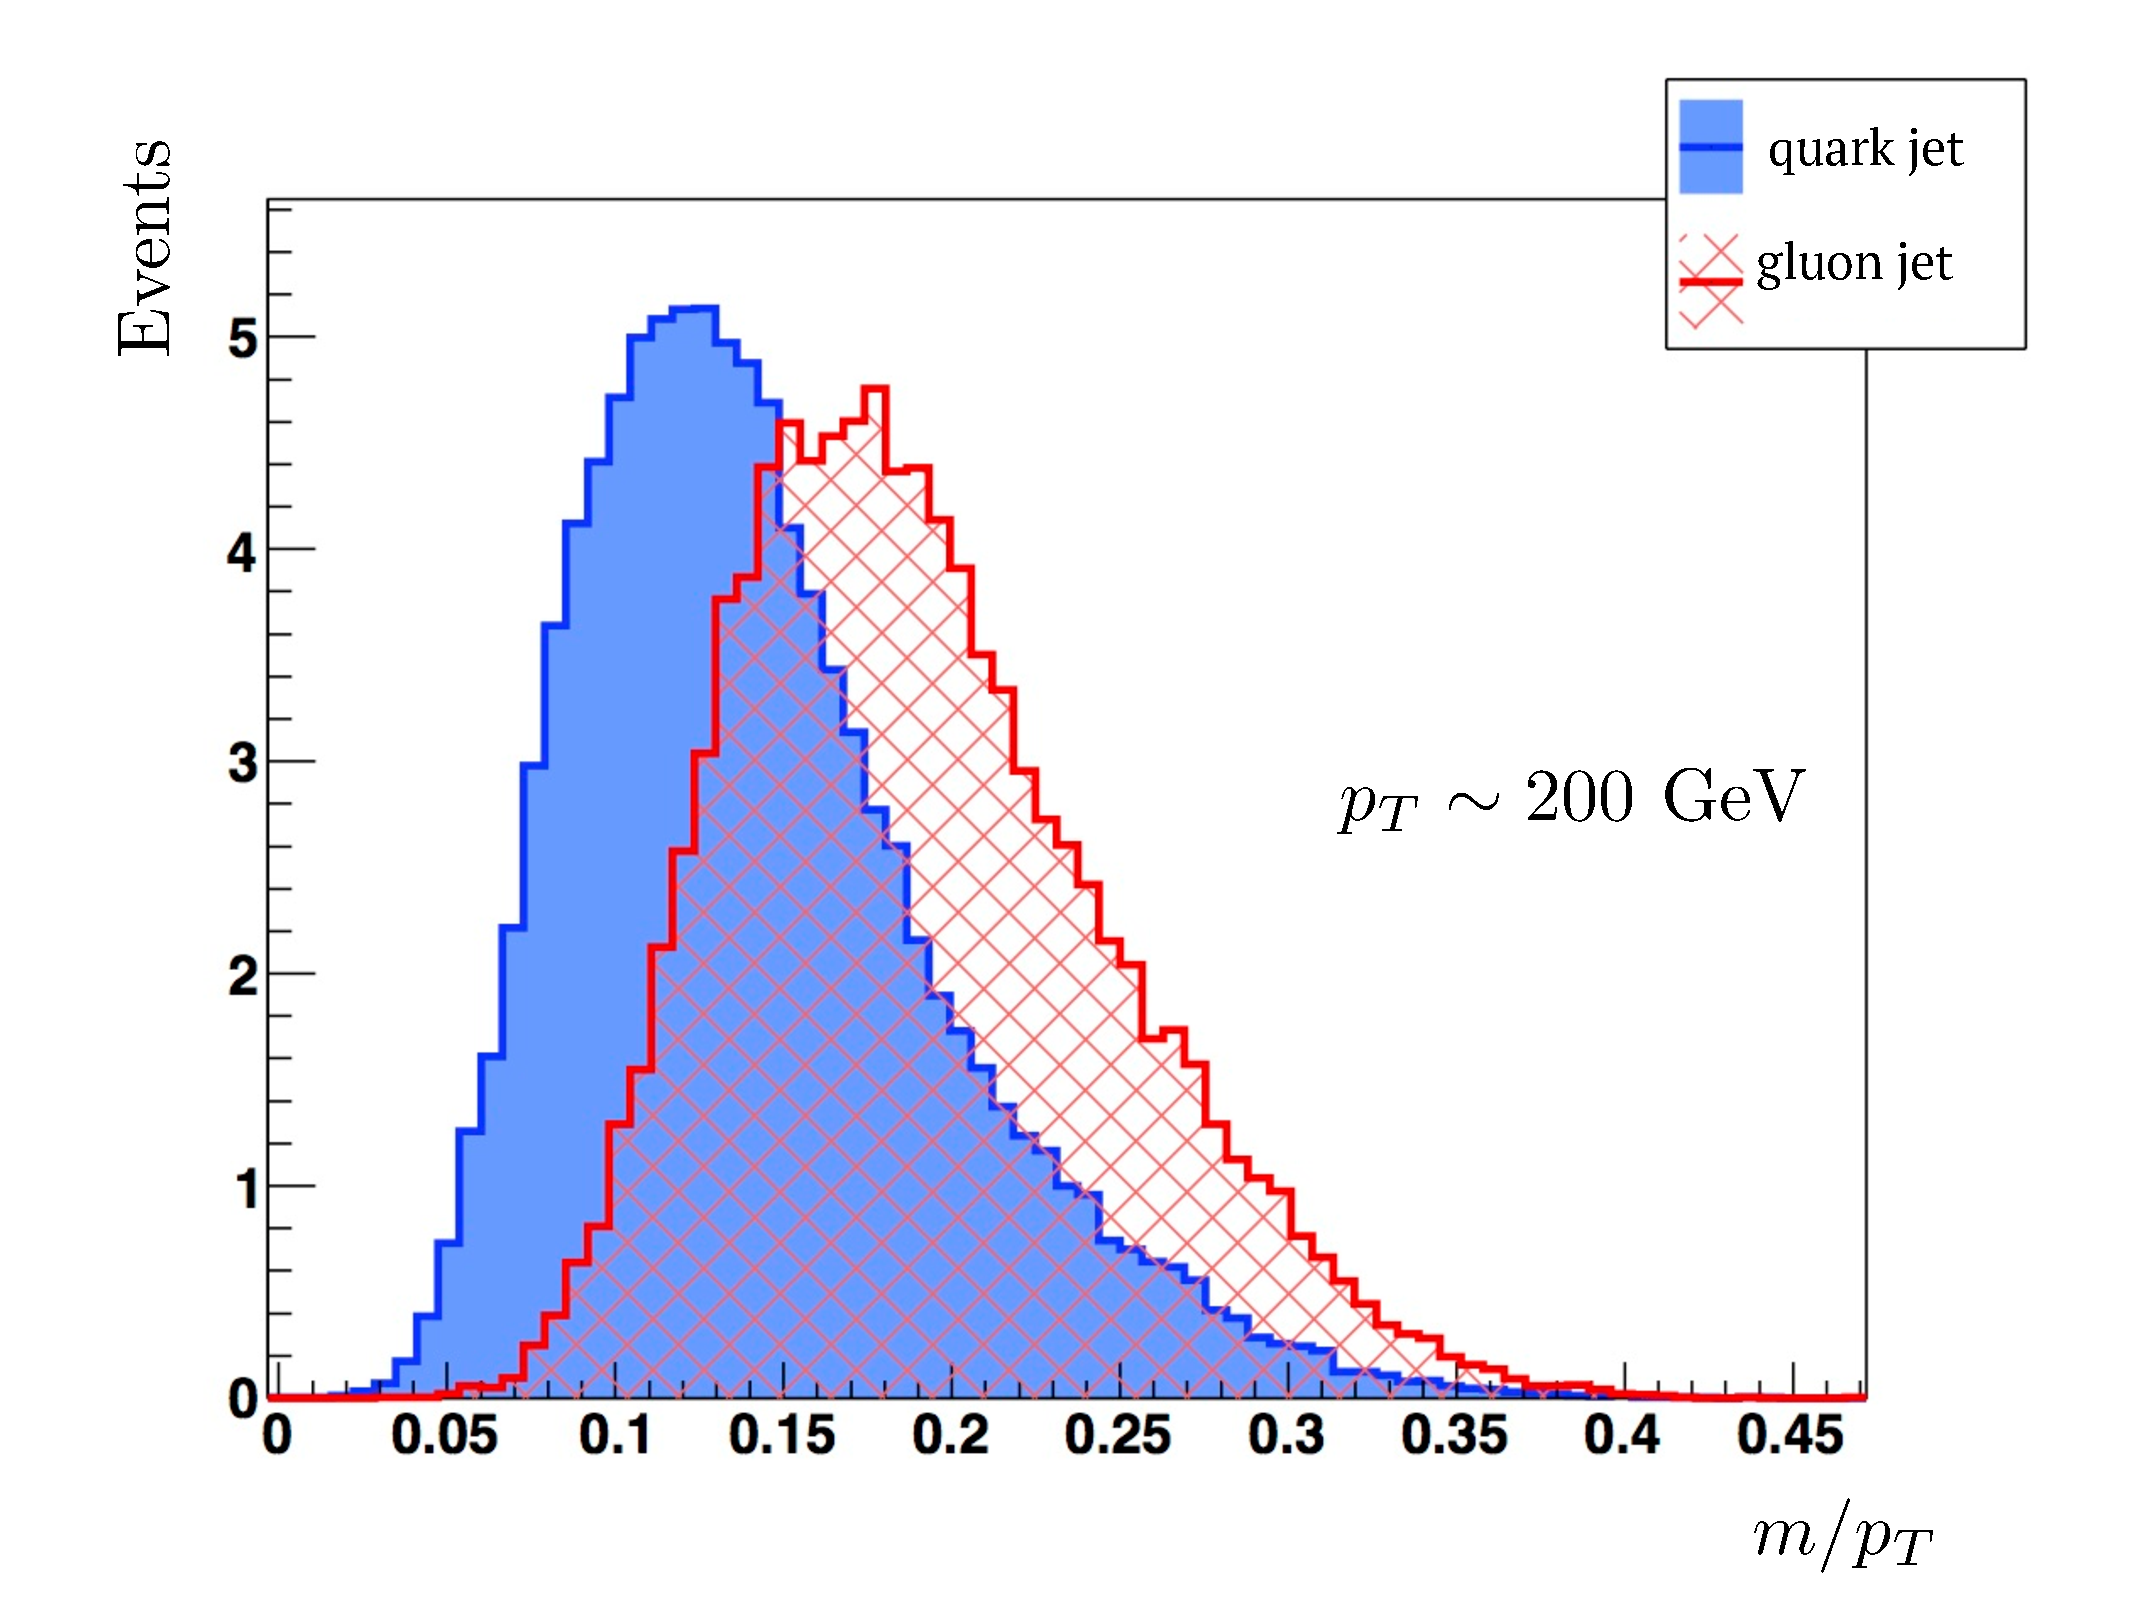
\includegraphics[width=0.49\textwidth]{figures/analysis/search2/misc/ak07_MDPt_0200.pdf}
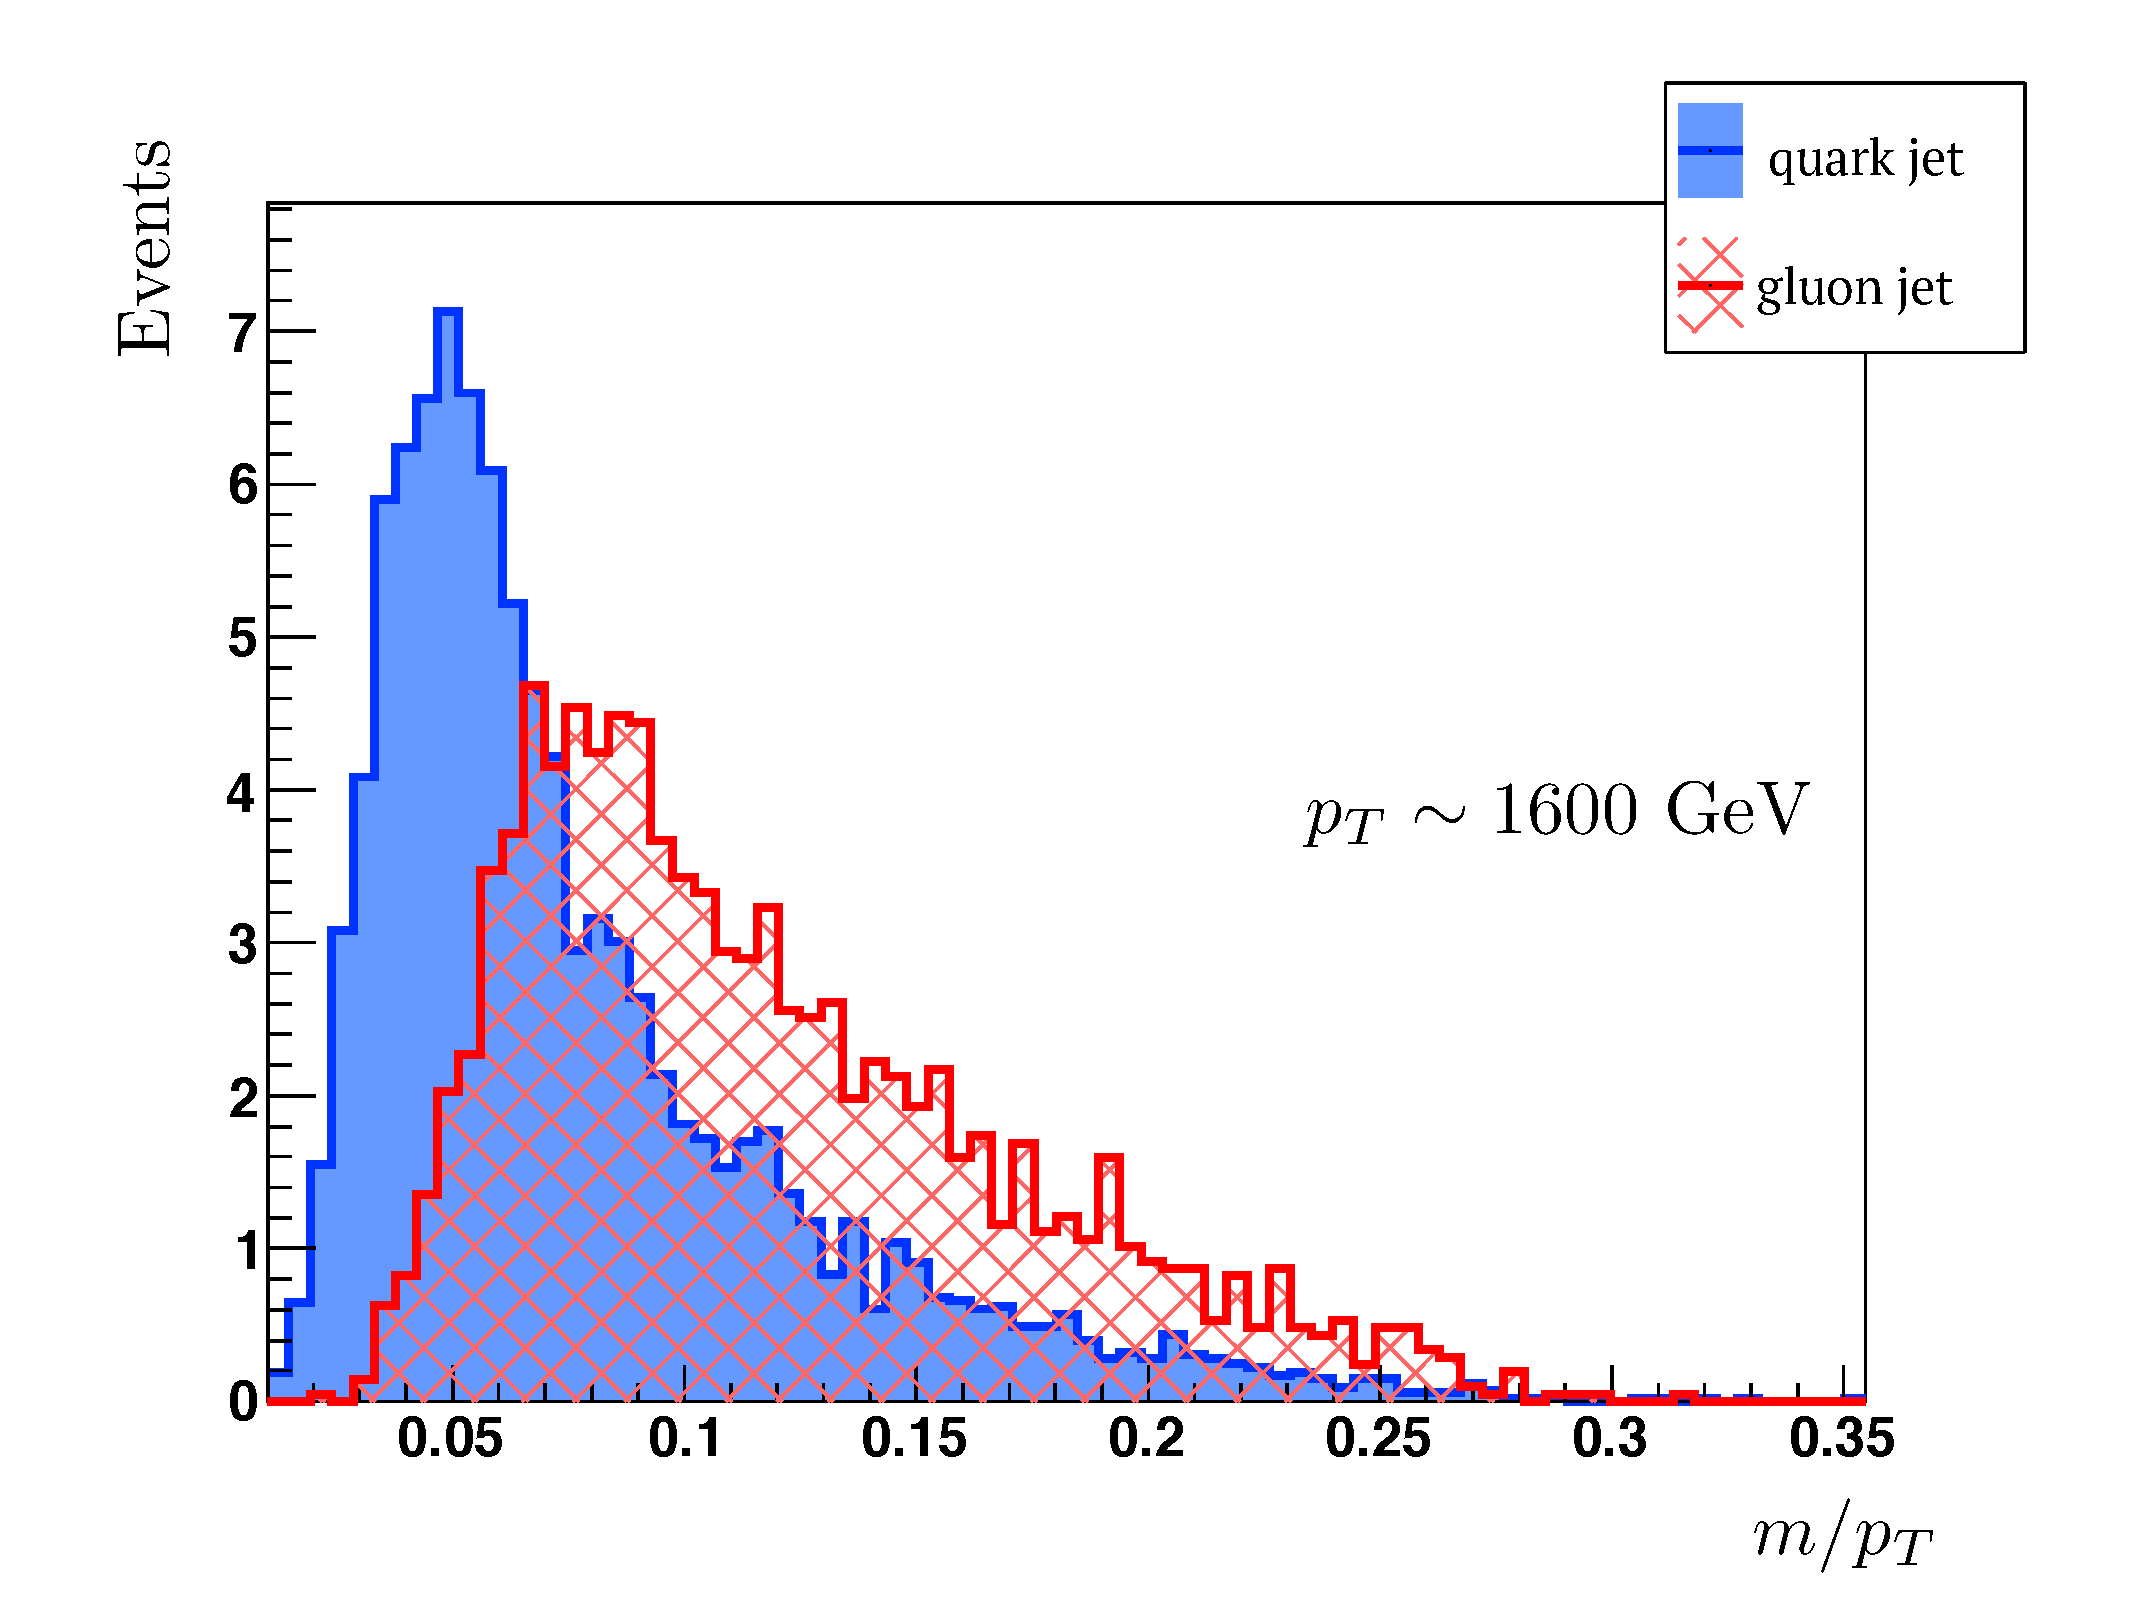
\includegraphics[width=0.49\textwidth]{figures/analysis/search2/misc/ak07_MDPt_1600.pdf}
\caption{The jet mass divided by the jet \PT for quark (blue) and gluon (red) jets for a jet \PT of 200 (left) and 1600 \GeV (right). Generated using~\cite{Gallicchio:2011xq}.}
\label{fig:searchII:mpt_qvsg}
\end{figure}
\clearpage

\section{Mass and purity categorization}
The PUPPI softdrop jet mass and PUPPI \nsubj distributions after loose analysis preselections, as outlined in Section~\ref{sec:searchII:samples},  have been applied are shown in Figure~\ref{fig:searchII:wtag}.
We see some disagreement between data and MC, especially in the high-purity region (PUPPI $\ddt<0.4$), confirming what was observed in Section~\ref{sec:searchII:wmistag}.
\begin{figure}[h!]
\centering
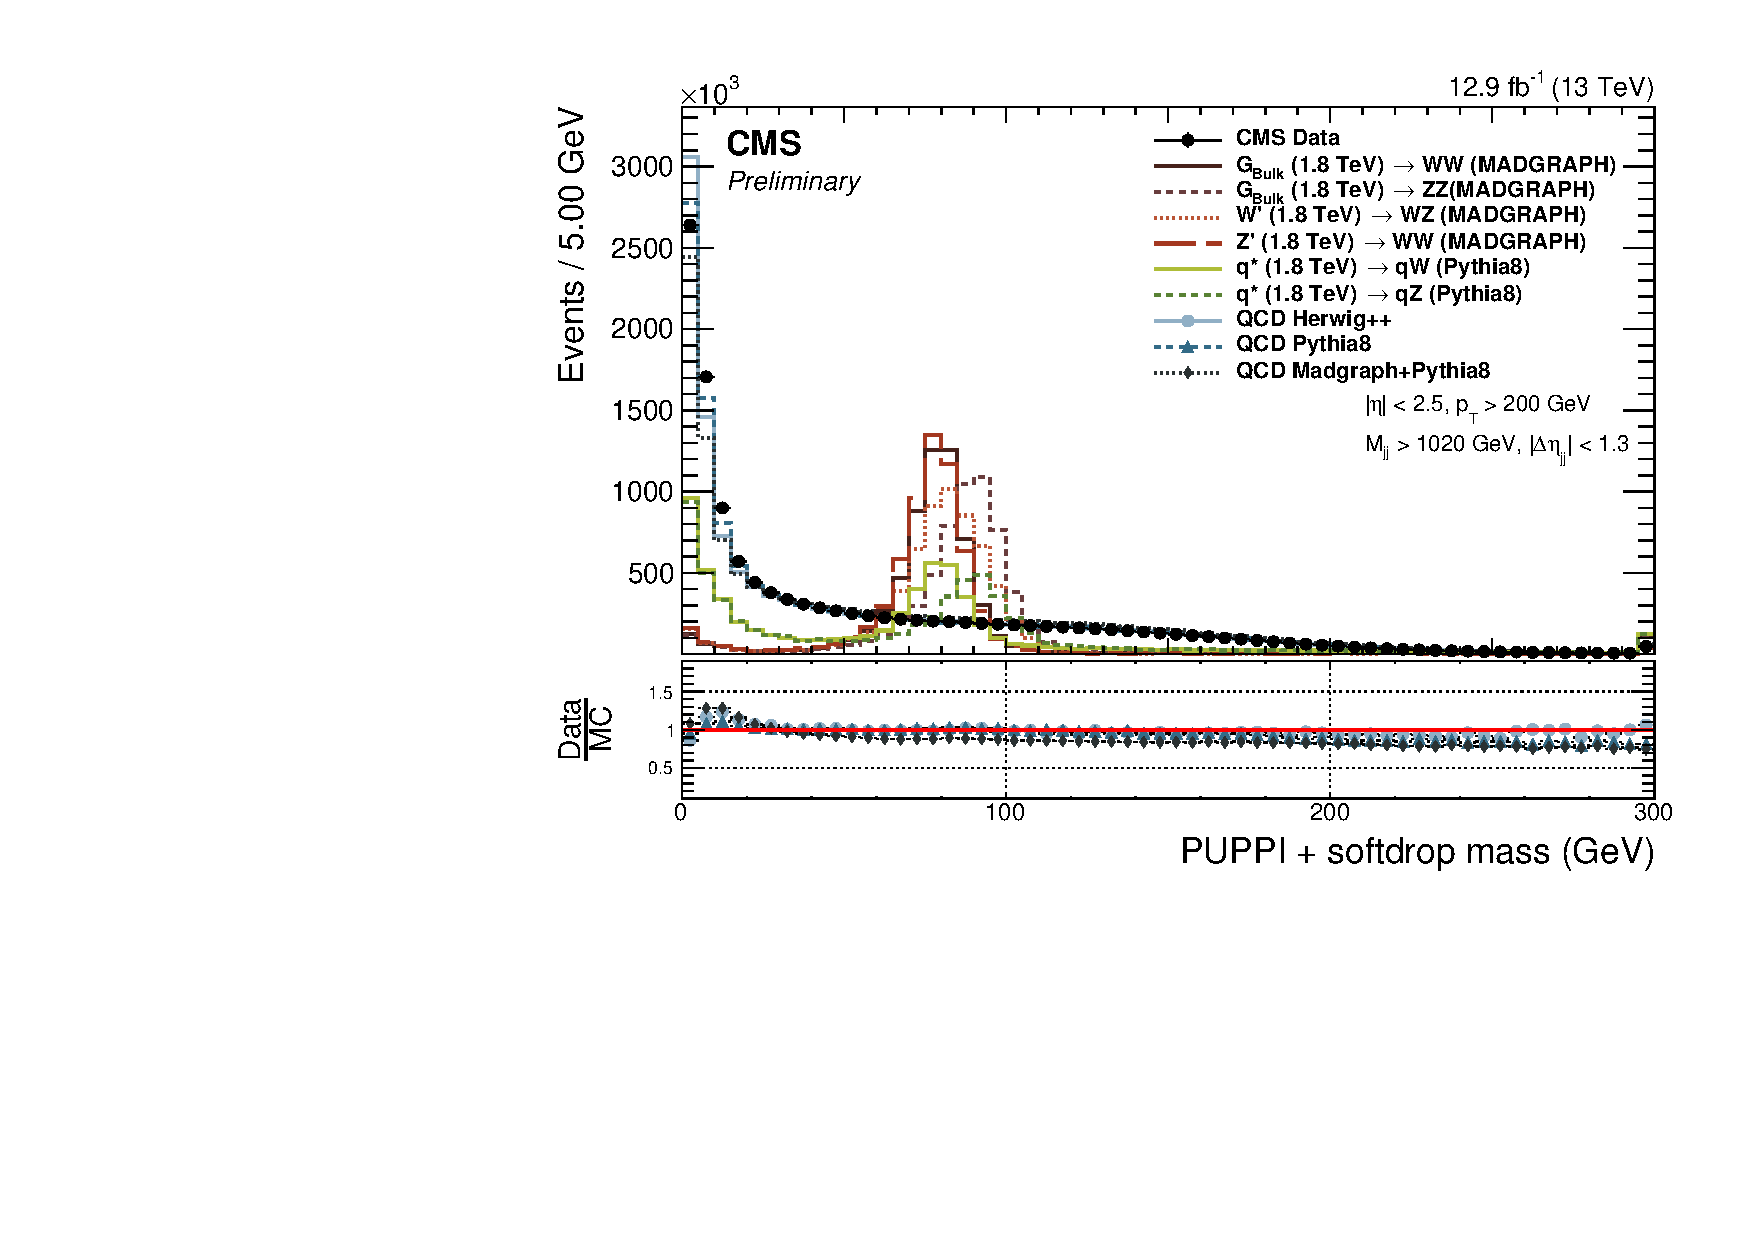
\includegraphics[width=0.49\textwidth]{figures/analysis/search2/AN-16-235/plots/qcdcp_PuppiSoftdropMass.pdf}
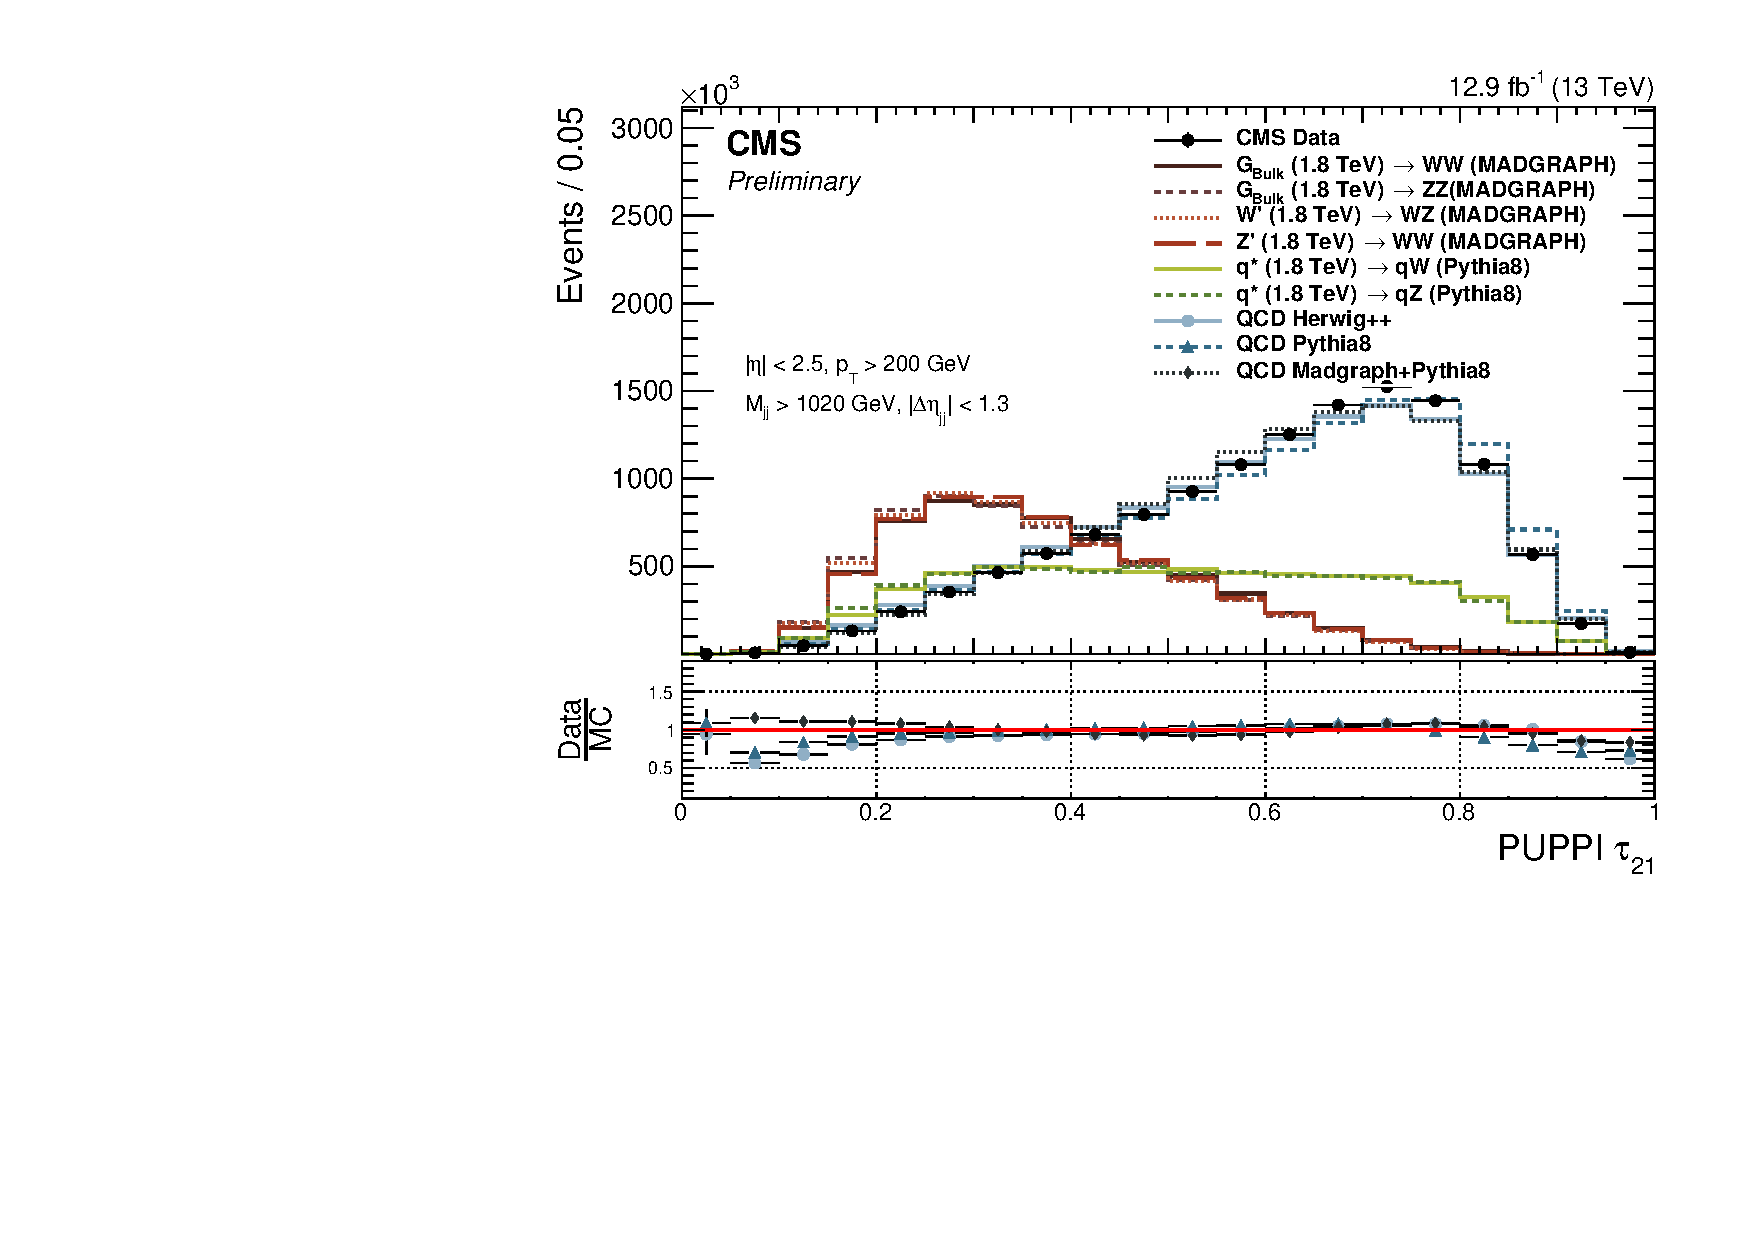
\includegraphics[width=0.49\textwidth]{figures/analysis/search2/AN-16-235/plots/qcdcp_puppi_tau2tau1.pdf}
\caption{PUPPI softdrop jet mass (left) and PUPPI n-subjettiness $\tau_{21}$ (right) distribution for data and simulated samples. Simulated samples are scaled to match the distribution in data.}
\label{fig:searchII:wtag}
\end{figure}
\noindent As this analysis is sensitive to both heavy resonances decaying into two vector bosons and excited quark resonances $q^*$ decaying to qW and qZ, we look for events with both a single V-tag and events with two V-tags. 
Vector boson candidates are selected with a PUPPI softdrop jet mass of $65 \GeV < m_{sd} <105 \GeV$. Further, and similar to what was done in Search I, we select "high-purity" (HP) W and Z jets by requiring PUPPI $0<\tau_{21} \leq 0.40$ and "low-purity" (LP) W and Z jets with $0.40<\tau_{21}\leq0.75$. The events with one W/Z-tag are classified in HP and LP categories according to the two categories described above. Events with two W/Z-tagged jets are always required to have one HP tagged jet, and are further divided into LP and HP categories depending on whether the other jet is of high or low purity. We additionally split events into two mass categories in order to enhance the analysis sensitivity, with the W-window defined as $65 \GeV < m_{sd} < 85 \GeV$ and the Z boson window as $85 \GeV < m_{sd} < 105 \GeV$. This results in ten different signal categories: for the double W/Z-tag analysis, there are 3 mass categories corresponding to WW, WZ, and ZZ for HP, and the same 3 mass categories for LP. For the single W/Z-tag analysis, there are 2 mass categories corresponding to qW and qZ in HP, and the same for LP.
\clearpage

\section{Background modeling} 
\label{sec:searchII:ftest}
The background is modeled using a parametric fit of the dijet invariant mass spectrum in the data signal region in the same way as described in Section~\ref{sec:searchI:bkg}. We determine the number of necessary fit parameters in order to describe the background through a Fishers F-test, comparing the same fit functions as in Section~\ref{sec:searchI:bkg}. This test is first exercised in QCD MC and then in a data sideband before the final determination is performed in the data signal region. As the F-test method was presented in detail in the context of Search I, only a brief summary of the findings as well as a presentation of the fits in the single-tag categories will be presented here. Fits and F-test results for all categories can be found in Appendix~\ref{app:2016xcheck}. A two- or three-parameter fit is sufficient to describe the background for all the double-tag categories: a two-parameter fit is sufficient for the "high-purity" WZ and ZZ categories, as well as the "low-purity" WW category, while the remaining analysis categories require a three-parameter background fit.
From the fits of the single-tag categories, shown in Figure~\ref{fig:searchII:bkgfit_sr_qv}, a three-parameter fit is sufficient for all categories except for the "high-purity" qW category. In the qW category, the improvement in fit quality when increasing the number
of parameters is so large that adding an additional fit parameter is justified, and we continue by using a 5-parameter fit for this category. 
\begin{figure}[h!]
\centering
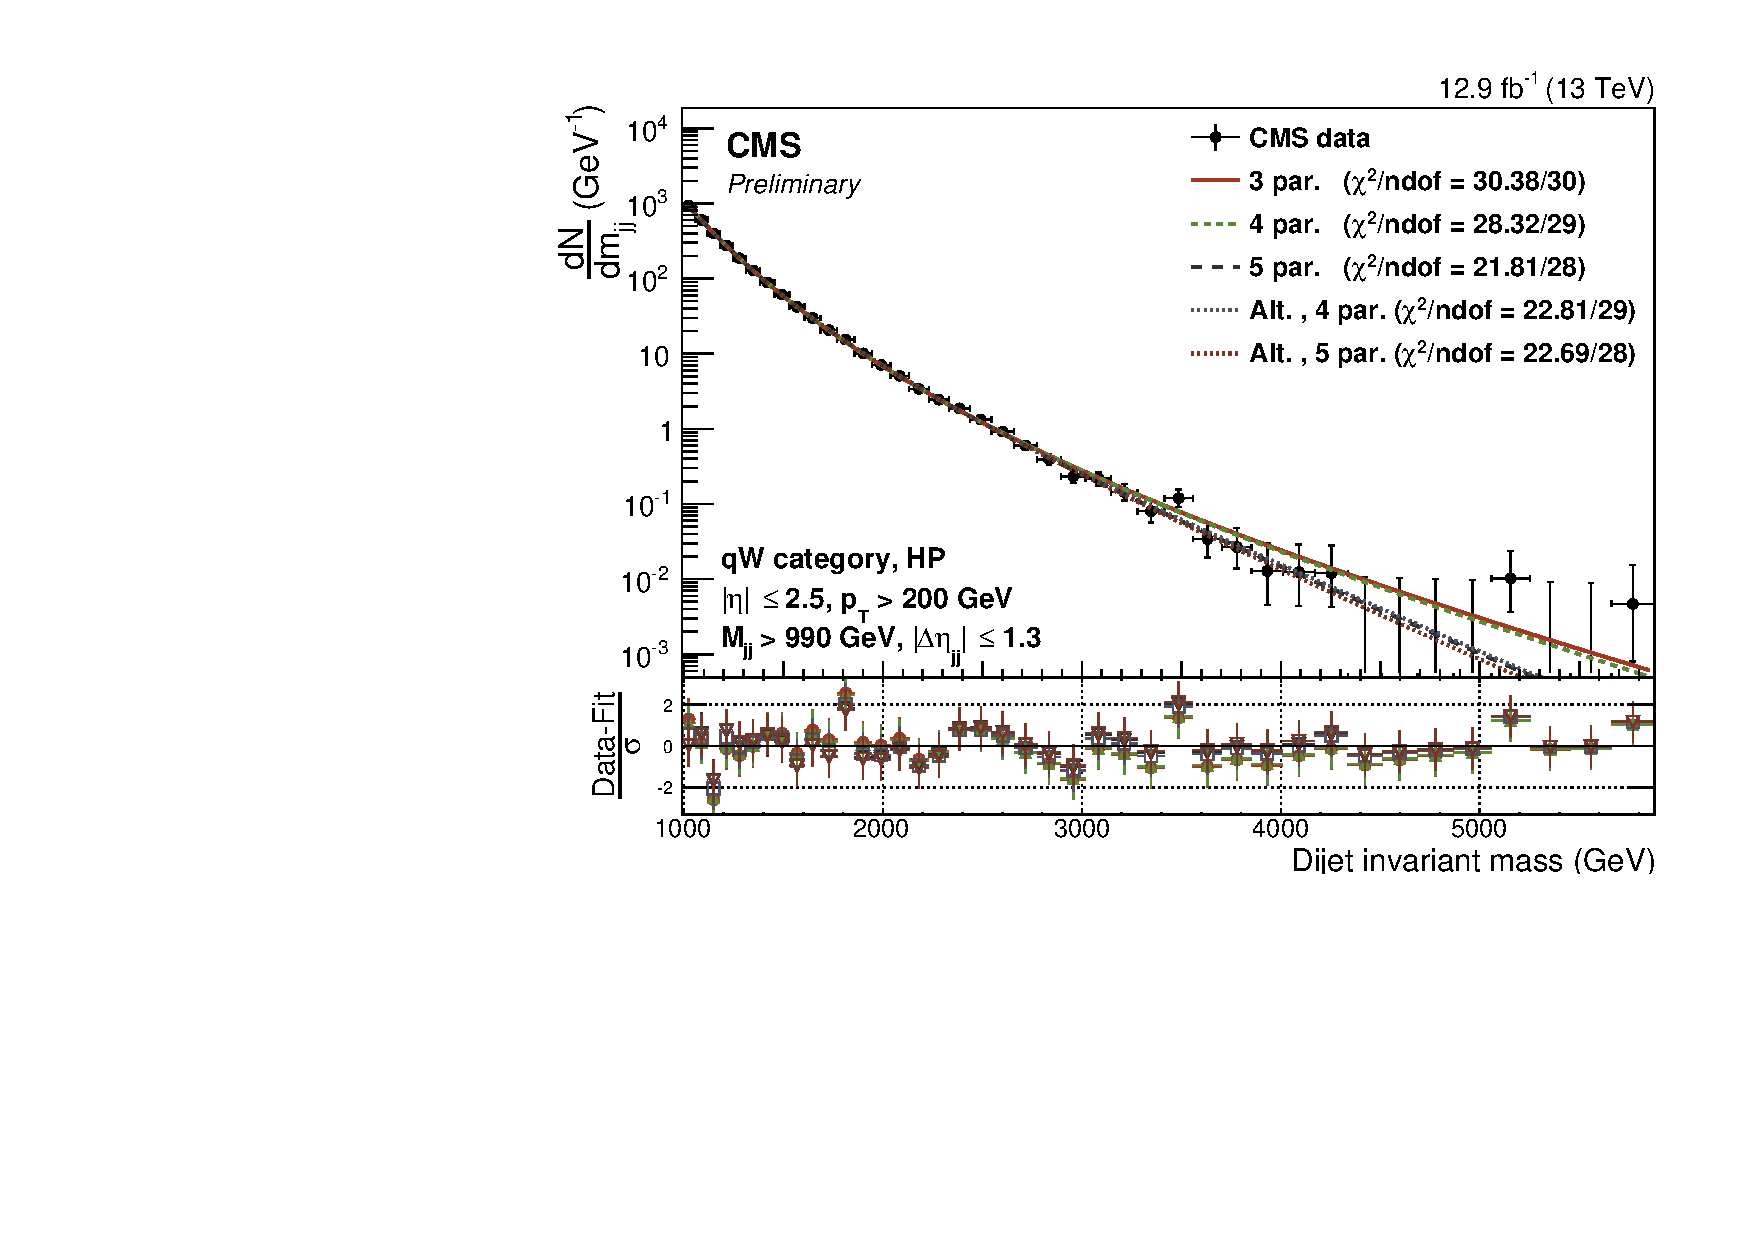
\includegraphics[width=0.45\textwidth]{figures/analysis/search2/AN-16-235/plots/qWHP.pdf}
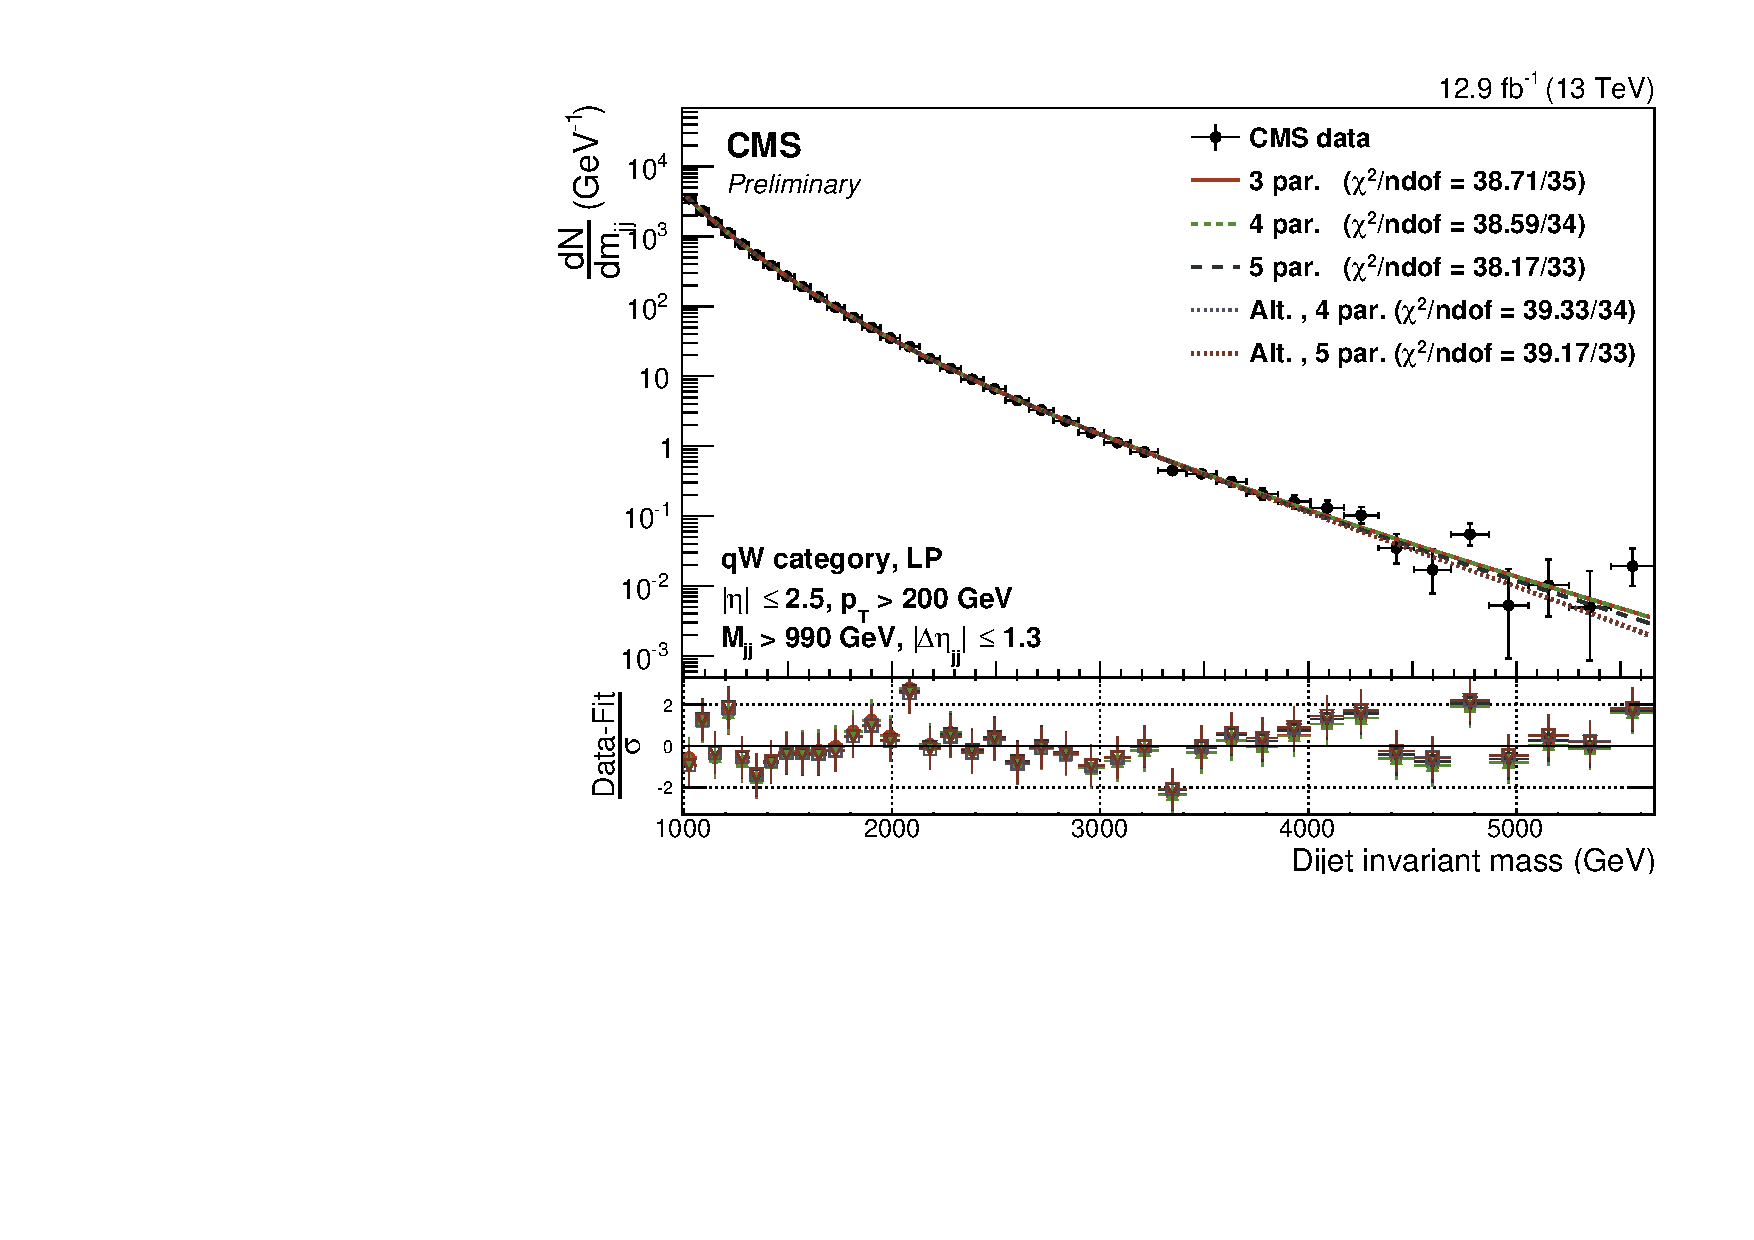
\includegraphics[width=0.45\textwidth]{figures/analysis/search2/AN-16-235/plots/qWLP.pdf}\\
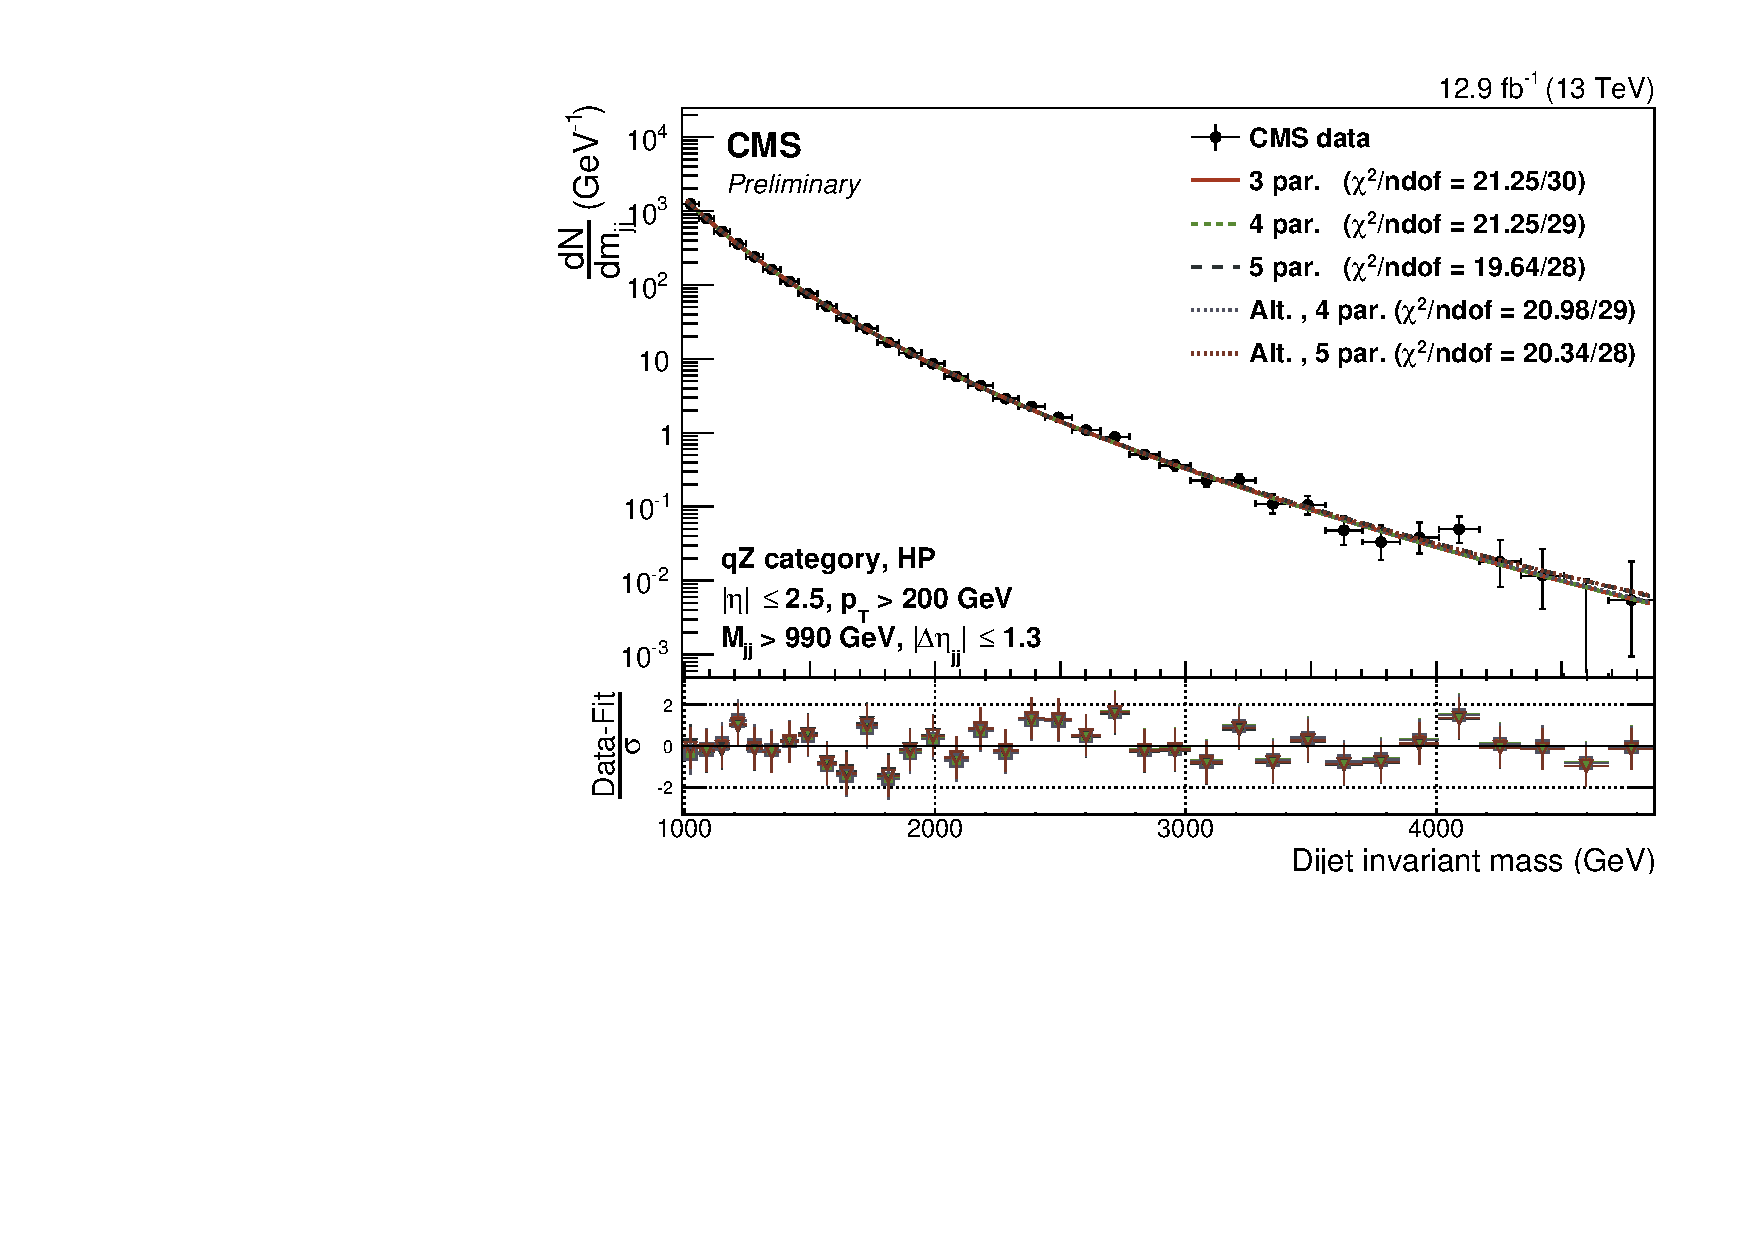
\includegraphics[width=0.45\textwidth]{figures/analysis/search2/AN-16-235/plots/qZHP.pdf}
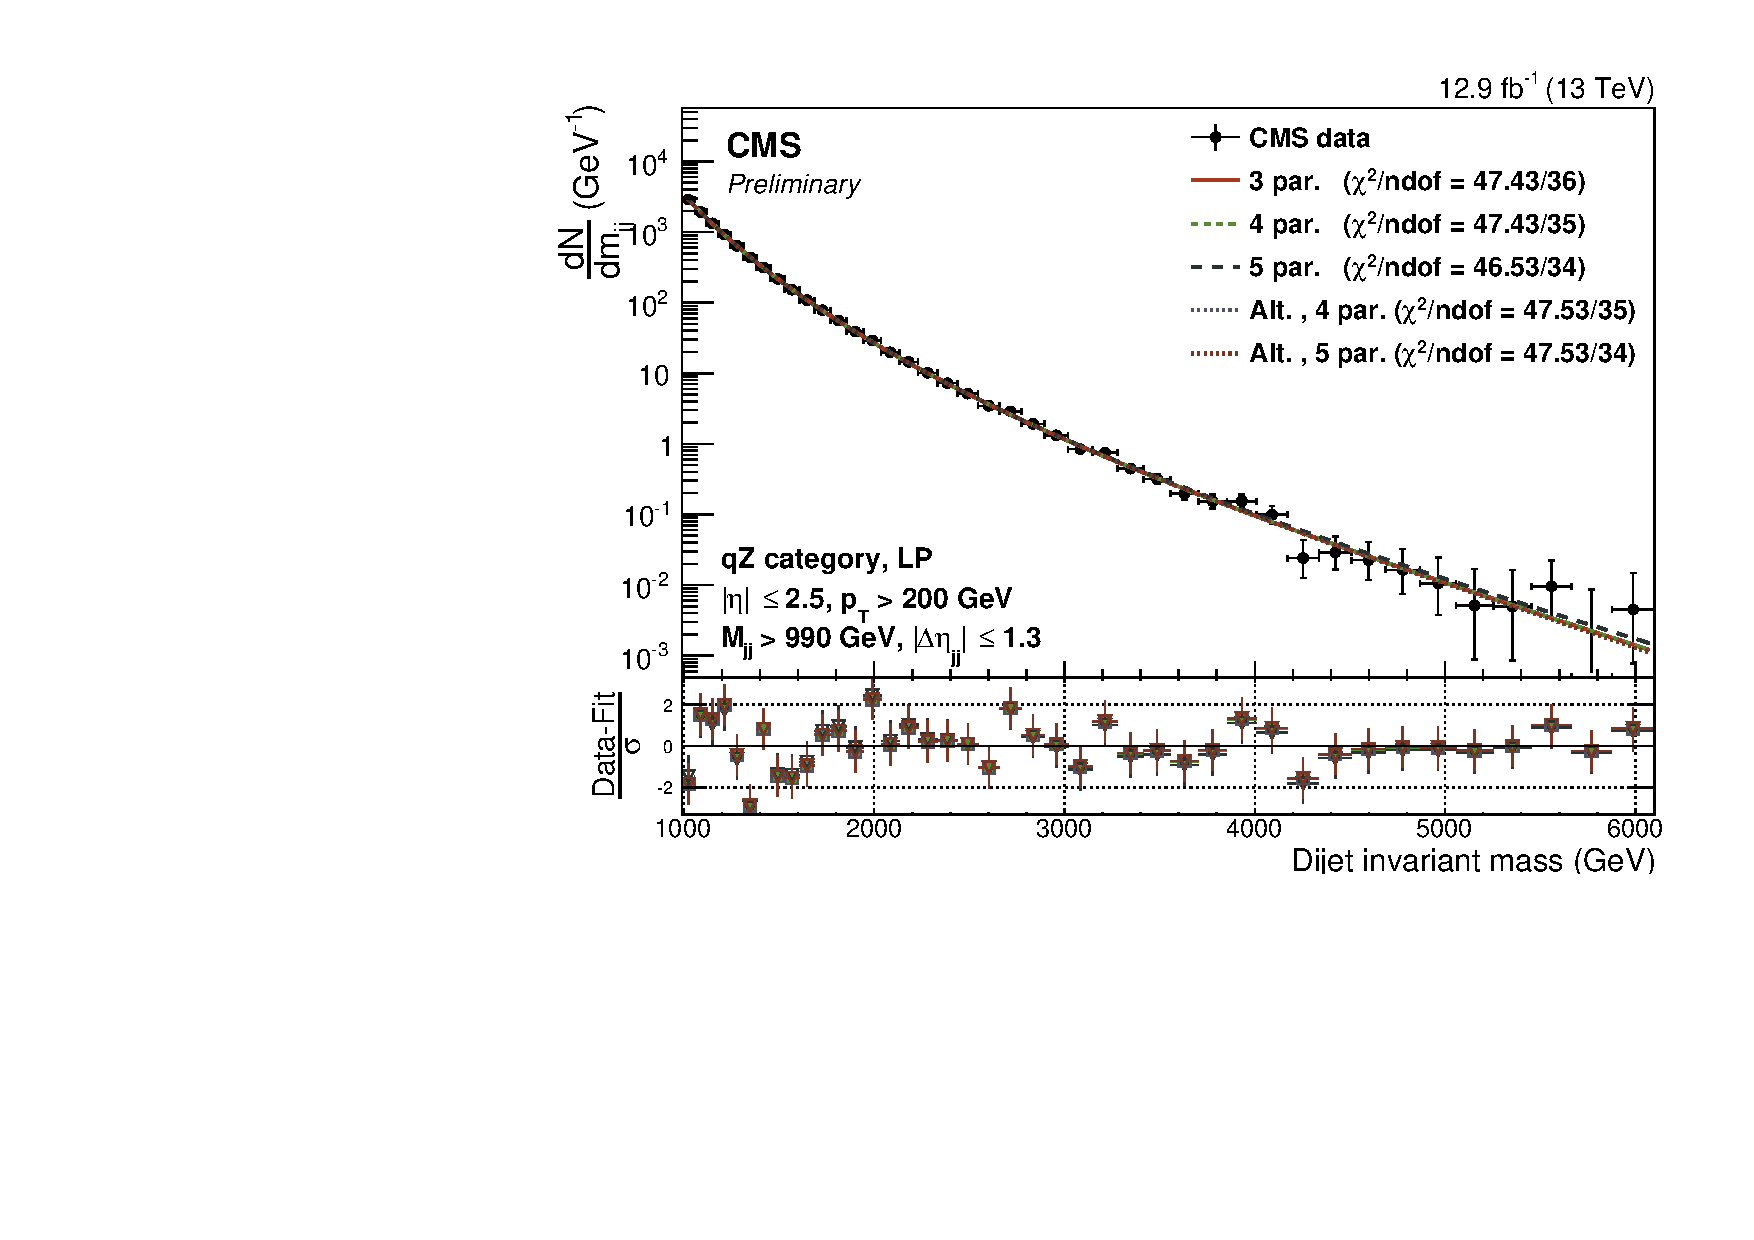
\includegraphics[width=0.45\textwidth]{figures/analysis/search2/AN-16-235/plots/qZLP.pdf}\\
\caption{Background-only fit of the dijet invariant mass distribution in the data signal region used to establish the number of parameters of the background shape for the single-tag analysis. Here for the high- (left) and low-purity (right) single V-tag categories qW (top) and qZ (bottom).}
\label{fig:searchII:bkgfit_sr_qv}
\end{figure}
A summary of what fit functions are used for each analysis category is listed in Table~\ref{tab:searchII:fitpars}.
\begin{table}[h!]
\centering
\begin{tabular}{|l| c | c|}
\hline
Mass category & \multicolumn{2}{|c|}{N pars.}\\
\hline
& HP & LP \\
\hline
WW & 3 & 2 \\
WZ & 2 & 3 \\
ZZ & 2 & 3 \\
qW & 5 & 3 \\
qZ & 3 & 3 \\
\hline
\end{tabular}
\caption{The number of fit parameters used in the background fit to the dijet invariant mass distribution for each analysis category as determined through an F-test.}
\label{tab:searchII:fitpars}
\end{table}
\clearpage
\section{Signal modeling}
The dijet invariant mass distribution for signal is modeled from MC in the same way as in Section~\ref{sec:searchI:sig}, where we assume the shape can be described by a Gaussian core and an exponential tail. The interpolated signal shapes for $\rm{q}^* \rightarrow \rm{q}\PW$ and $\rm{q}^* \rightarrow \rm{q}\PZ$ in their most sensitive analysis categories ($\rm{q}\PW$ and $\rm{q}\PZ$, respectively) are shown in Figure \ref{fig:searchII:interpolation}. The signal shapes for the double-tag categories can be compared to those in Figure~\ref{fig:searchI:sigfit}.
\begin{figure}[h!]
\centering
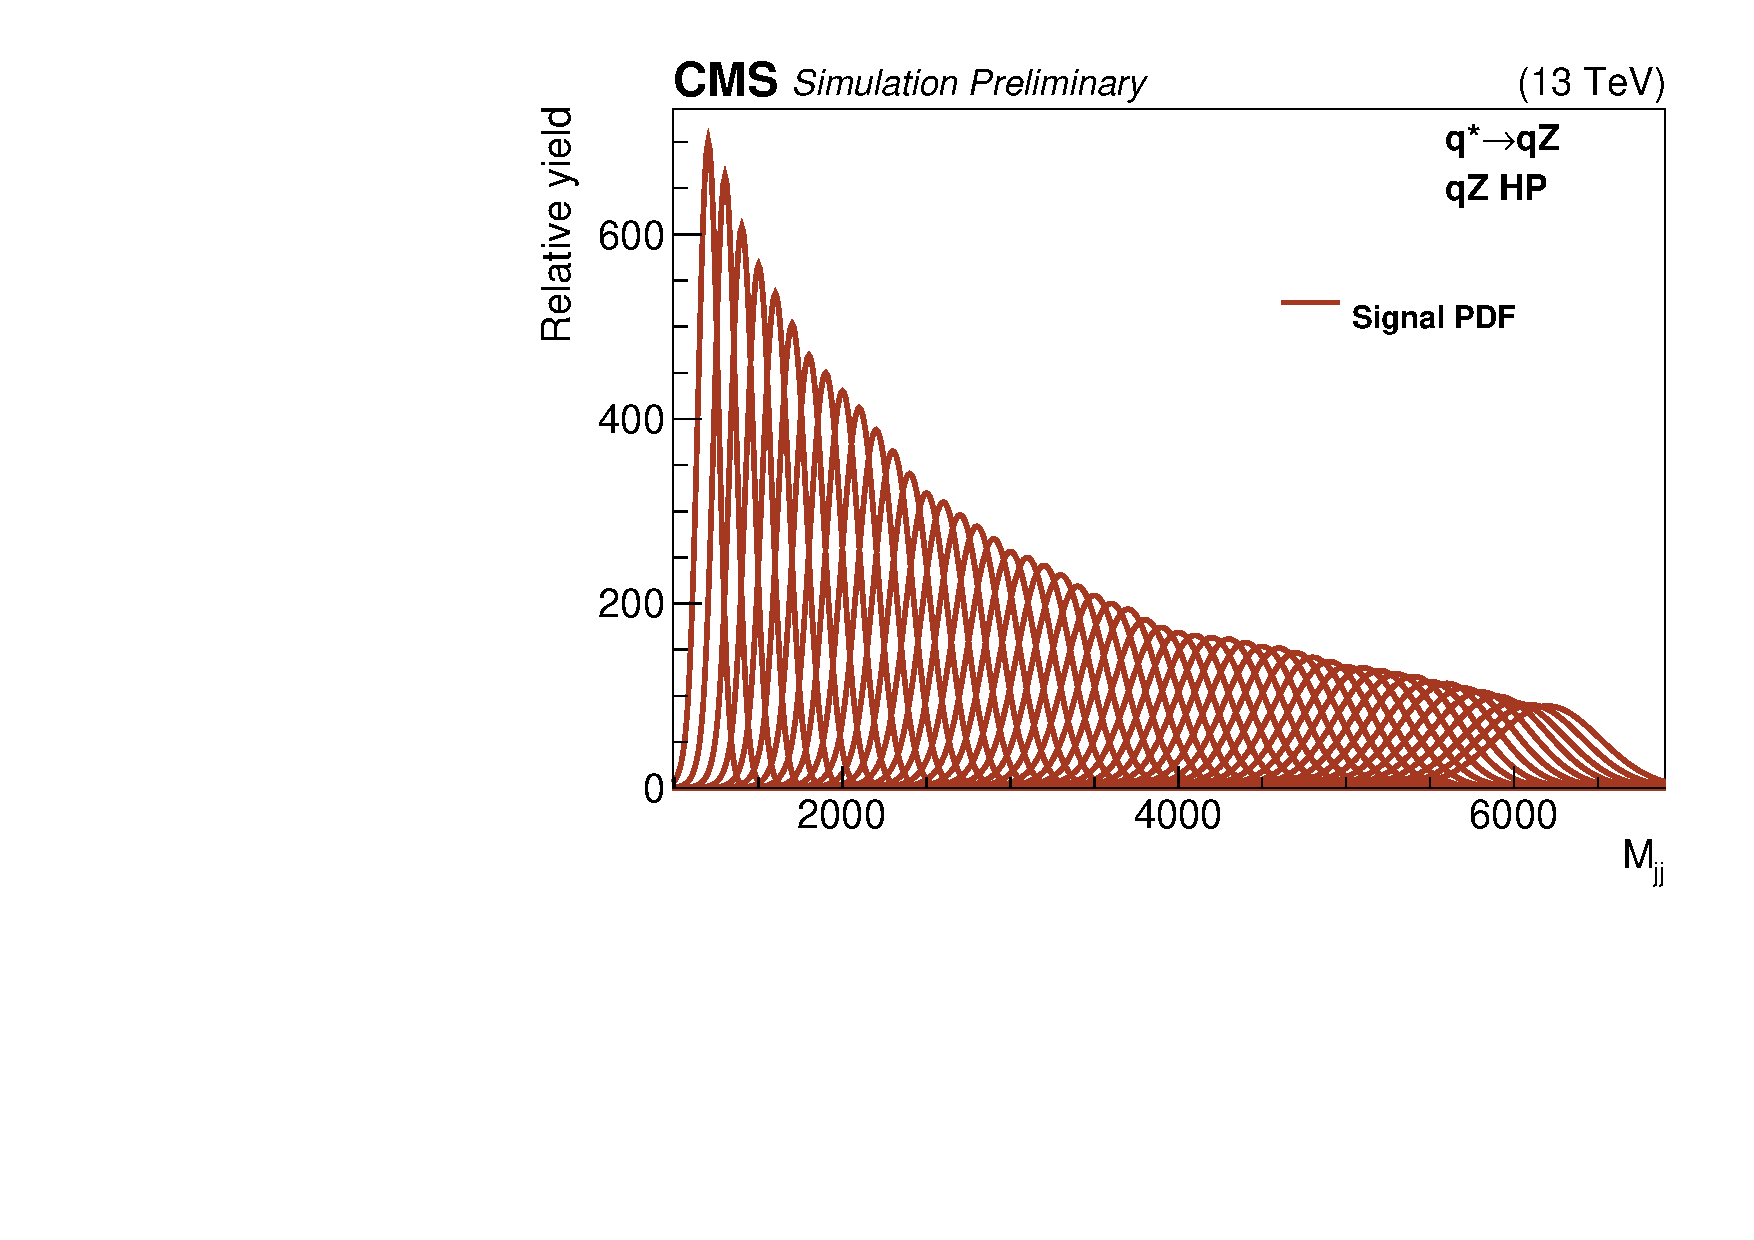
\includegraphics[width=0.49\textwidth]{figures/analysis/search2/AN-16-235/plots/interpolation_QstarQZ_DijetMassHighPuriqZ.pdf}
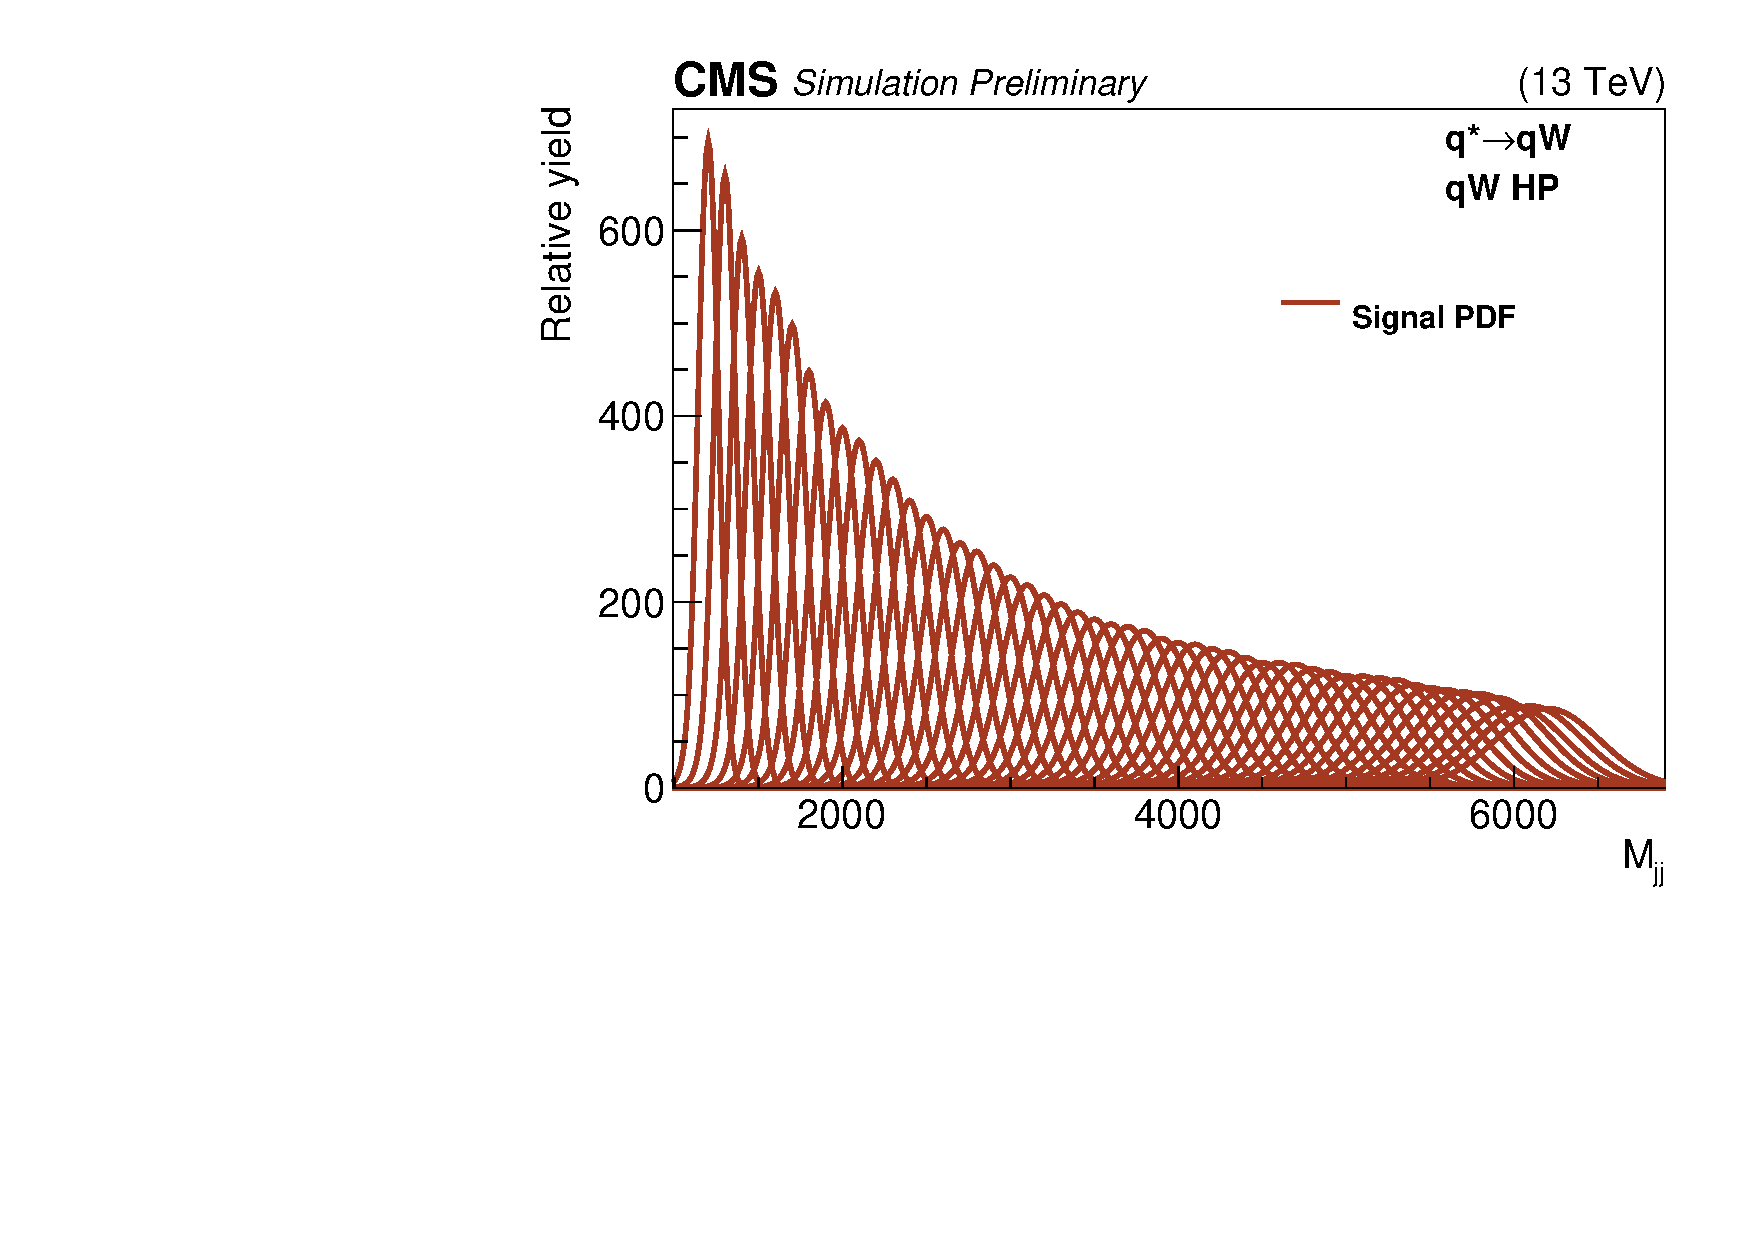
\includegraphics[width=0.49\textwidth]{figures/analysis/search2/AN-16-235/plots/interpolation_QstarQW_DijetMassHighPuriqW.pdf}\\
\caption{Interpolated signal shapes for a  $q^*\rightarrow qZ$ (left) and $q^*\rightarrow qW$ (right) signal.}
\label{fig:searchII:interpolation}
\end{figure}
\clearpage
\section{Systematic uncertainties}
The largest sources of systematic uncertainty for this analysis are, as for Search I, related to the signal modeling and are due to the uncertainty in the tagging efficiency of the V-tagger, the jet energy an mass scale, the jet energy and mass resolution and the integrated luminosity. The V-tagging uncertainty is estimated as described in Section~\ref{sec:searchII:wtagsf}, and yield uncertainties on the scale factors for the HP and LP tagging categories.
The \pt- and $\eta$-dependent jet energy scale and resolution uncertainties on the resonance shape are approximated by a constant 2\% and 10\%. The jet energy scale and resolution uncertainty are taken into account as shape uncertainties by shifting and widening the signal resonance model,
while all other signal uncertainties only affect the yield. The most relevant systematic uncertainties are listed in Table~\ref{tab:searchII:VV_systematicssummary_signal}.
\begin{table}[h!]
  \centering
  \begin{tabular}{lccc}
    \hline
    Source                        & Relevant quantity      & HP+HP unc. (\%)  & HP+LP unc. (\%)\\
    \hline
    Jet energy scale                 & Resonance shape        & 2                    & 2 \\
    Jet energy resolution            & Resonance shape        & 10                   & 10 \\
    \hline
    Jet energy scale                 & Signal yield           & \multicolumn{2}{c}{$<$0.1--4.4}\\ 
    Jet energy resolution            & Signal yield           & \multicolumn{2}{c}{$<$0.1--1.1}\\
    Jet mass scale                   & Signal yield           & \multicolumn{2}{c}{0.02--1.5}\\ 
    Jet mass resolution              & Signal yield           & \multicolumn{2}{c}{1.3--6.8}\\ 
    Pileup                           & Signal yield           & \multicolumn{2}{c}{2}\\
    Integrated luminosity            & Signal yield           & \multicolumn{2}{c}{6.2}\\
    PDFs (\PWpr)                     & Signal yield		       & \multicolumn{2}{c}{4--19}\\
    PDFs (\PZpr)                     & Signal yield		       & \multicolumn{2}{c}{4--13}\\
    PDFs (\BulkG)                    & Signal yield		       & \multicolumn{2}{c}{9--77}\\
    Scales (\PWpr)                   & Signal yield		       & \multicolumn{2}{c}{1--14}\\
    Scales (\PZpr)                   & Signal yield		       & \multicolumn{2}{c}{1--13}\\
    Scales (\BulkG)                  & Signal yield		       & \multicolumn{2}{c}{8--22}\\
    \hline
    % Jet energy scale                 & Migration              & \multicolumn{2}{c}{0--14}\\
%     Jet energy resolution            & Migration              & \multicolumn{2}{c}{0--4.1}\\
    Jet mass scale                   & Migration              & \multicolumn{2}{c}{$<$0.1--16.8}\\
    Jet mass resolution              & Migration              & \multicolumn{2}{c}{$<$0.1--17.8}\\
    W-tagging \nsubj{}               & Migration              & 15.6                  & 21.9\\
    W-tagging \pt-dependence         & Migration              & 7--14                 & 5--11\\
    \hline
  \end{tabular}
  \caption{Summary of the systematic uncertainties on the signal and their impact on the event yield in the signal region and on the reconstructed dijet invariant mass shape (mean and width).}
  \label{tab:searchII:VV_systematicssummary_signal}
\end{table}

\section{Results}   
As mentioned in the introduction to this chapter, the analysis of the 2016 dataset was done in two steps: one based on 12.9 \fbinv of data collected early in 2016, demonstrating the new PUPPI softdrop V-tagger and the new single-tag analysis categories, and one utilizing the full 35.9 \fbinv of data collected in 2016. The results from both will be presented in the following sections.

\subsection{Early analysis}   
\label{sec:searchII:b2g16021res}
The dijet invariant mass distributions in the analysis signal regions using 12.9 \fbinv of data collected in 2016, are shown in Figure~\ref{fig:searchII:doubleobsmvv} for the double-tag and in Figure~\ref{fig:searchII:doubleobsmqv} for the single-tag analysis. No significant excess is observed and we proceed to set upper limits on the signal cross section using the method described in Section~\ref{sec:searchI:results}.
\begin{figure}[h!]
\centering
\includegraphics[width=0.45\textwidth]{figures/analysis/search2/B2G-16-021/figures/mjj/MLBkgFit_DijetMassHighPuriWW.pdf}
\includegraphics[width=0.45\textwidth]{figures/analysis/search2/B2G-16-021/figures/mjj/MLBkgFit_DijetMassLowPuriWW.pdf}\\
\includegraphics[width=0.45\textwidth]{figures/analysis/search2/B2G-16-021/figures/mjj/MLBkgFit_DijetMassHighPuriWZ.pdf}
\includegraphics[width=0.45\textwidth]{figures/analysis/search2/B2G-16-021/figures/mjj/MLBkgFit_DijetMassLowPuriWZ.pdf}\\
\includegraphics[width=0.45\textwidth]{figures/analysis/search2/B2G-16-021/figures/mjj/MLBkgFit_DijetMassHighPuriZZ.pdf}
\includegraphics[width=0.45\textwidth]{figures/analysis/search2/B2G-16-021/figures/mjj/MLBkgFit_DijetMassLowPuriZZ.pdf}
\caption{Observed dijet invariant mass spectrum for the double-tag analysis in the high-purity (left) and low-purity (right) categories using 12.9 \fbinv of data collected in 2016.}
\label{fig:searchII:doubleobsmvv}
\end{figure}
\begin{figure}[h!]
\centering
\includegraphics[width=0.45\textwidth]{figures/analysis/search2/B2G-16-021/figures/mjj/MLBkgFit_DijetMassHighPuriqW.pdf}
\includegraphics[width=0.45\textwidth]{figures/analysis/search2/B2G-16-021/figures/mjj/MLBkgFit_DijetMassHighPuriqZ.pdf}\\
\includegraphics[width=0.45\textwidth]{figures/analysis/search2/B2G-16-021/figures/mjj/MLBkgFit_DijetMassLowPuriqW.pdf}
\includegraphics[width=0.45\textwidth]{figures/analysis/search2/B2G-16-021/figures/mjj/MLBkgFit_DijetMassLowPuriqZ.pdf}
\caption{Observed dijet invariant mass spectrum for the single-tag analysis in the high-purity (top) and low-purity (bottom) categories using 12.9 \fbinv of data collected in 2016.}
\label{fig:searchII:doubleobsmqv}
\end{figure}
\noindent Exclusion limits are set in the context of the bulk graviton model, the HVT model~B, and excited-quark resonance models,
assuming the resonances have a natural width negligible with respect to the experimental resolution (as in Search I). Figure~\ref{fig:searchII:limitCombined} shows the expected and observed upper exclusion limits at 95\% confidence level (CL) on the signal cross section times the branching fraction as a function of the resonance mass for the different signal hypotheses in the double-tag analysis. The limits are compared with the theoretically predicted cross section times branching fraction to $\PW\PW$ and $\PZ\PZ$ for a bulk graviton with $\ktilde = 0.5$, and with the cross section
times branching fraction to $\PW\PZ$ and $\PW\PW$ for spin-1 particles predicted by the HVT model~B. For the HVT model B, we exclude \PWpr (\PZpr) resonances with masses below 2.7 (2.6)~\TeV. The signal cross section uncertainties are displayed as a red checked band and result in an additional uncertainty on the resonance mass limits of 0.05 (0.04)~\TeV.
The cross section limits for $\PZpr \rightarrow \PW\PW$ and $\rm G_{bulk}\rightarrow\PW\PW$ are not identical due to the different acceptance for those two signal scenarios.
\begin{figure}[h!]
\centering
     \includegraphics[width=0.45\textwidth]{figures/analysis/search2/B2G-16-021/figures/limits/brazilianFlag_ZprimeWW_new_combined_13TeV.pdf}
     \includegraphics[width=0.45\textwidth]{figures/analysis/search2/B2G-16-021/figures/limits/brazilianFlag_WZ_new_combined_13TeV.pdf}\\
     \includegraphics[width=0.45\textwidth]{figures/analysis/search2/B2G-16-021/figures/limits/brazilianFlag_BulkWW_new_combined_13TeV.pdf}
     \includegraphics[width=0.45\textwidth]{figures/analysis/search2/B2G-16-021/figures/limits/brazilianFlag_BulkZZ_new_combined_13TeV.pdf}
\caption{Observed (black solid) and expected (black dashed) 95\% CL upper limits on the production of a narrow-width resonance decaying to a pair of vector bosons for different signal hypotheses. Limits are set in the context of a spin-1 neutral \PZpr (left) and charged \PWpr (right) resonance, and compared with the prediction of the HVT model~B. On the bottom, limits are set in the context of a bulk graviton decaying into $\PW\PW$ (left) and $\PZ\PZ$ (right) with $\ktilde =0.5$ and compared with the model prediction. Signal cross section uncertainties are displayed as a red checked band.}
\label{fig:searchII:limitCombined}
\end{figure}
\noindent Figure~\ref{fig:searchII:limitCombined_qV} shows the corresponding exclusion limits for excited quarks decaying to qW and qZ, excluding a $q^*$ decaying into qW and qZ with masses below 5.0 and 3.9~\TeV, respectively. The signal cross section uncertainties are displayed as a red checked band and result in an additional uncertainty on the resonance mass limits of 0.1~\TeV.
\begin{figure}[h!]
\centering
     \includegraphics[width=0.45\textwidth]{figures/analysis/search2/B2G-16-021/figures/limits/brazilianFlag_qW_new_combined_13TeV.pdf}
     \includegraphics[width=0.45\textwidth]{figures/analysis/search2/B2G-16-021/figures/limits/brazilianFlag_qZ_new_combined_13TeV.pdf}\\
\caption{Observed (black solid) and expected (black dashed) 95\% CL upper limits on the production of an excited quark resonance
decaying into qW (left) or qZ (right). Signal cross section uncertainties are displayed as a red checked band.}
\label{fig:searchII:limitCombined_qV}
\end{figure}
\subsection{Full 2016 dataset}   
\label{sec:searchII:brg17001res}
Figure~\ref{fig:searchII:doubleobsmvv_full} shows the dijet invariant mass distributions in the analysis signal regions using the full dataset of 35.9 \fbinv collected in 2016 for the double-tag and in Figure~\ref{fig:searchII:doubleobsmqv_full} for the single-tag analysis. No significant excess is observed and we proceed with setting upper limits on the signal cross section times branching ratio as in Section~\ref{sec:searchI:results}.\newline
\begin{figure}[h!]
\centering
\includegraphics[width=0.45\textwidth]{figures/analysis/search2/B2G-17-001/Figure_004-a.pdf}
\includegraphics[width=0.45\textwidth]{figures/analysis/search2/B2G-17-001/Figure_004-b.pdf}\\
\includegraphics[width=0.45\textwidth]{figures/analysis/search2/B2G-17-001/Figure_004-c.pdf}
\includegraphics[width=0.45\textwidth]{figures/analysis/search2/B2G-17-001/Figure_004-d.pdf}\\
\includegraphics[width=0.45\textwidth]{figures/analysis/search2/B2G-17-001/Figure_004-e.pdf}
\includegraphics[width=0.45\textwidth]{figures/analysis/search2/B2G-17-001/Figure_004-f.pdf}
\caption{Observed dijet invariant mass spectrum for the double-tag analysis in the high-purity (left) and low-purity (right) categories using 35.9 \fbinv of data collected in 2016.}
\label{fig:searchII:doubleobsmvv_full}
\end{figure}
\begin{figure}[h!]
\centering
\includegraphics[width=0.45\textwidth]{figures/analysis/search2/B2G-17-001/Figure_005-a.pdf}
\includegraphics[width=0.45\textwidth]{figures/analysis/search2/B2G-17-001/Figure_005-c.pdf}\\
\includegraphics[width=0.45\textwidth]{figures/analysis/search2/B2G-17-001/Figure_005-b.pdf}
\includegraphics[width=0.45\textwidth]{figures/analysis/search2/B2G-17-001/Figure_005-d.pdf}
\caption{Observed dijet invariant mass spectrum for the single-tag analysis in the high purity (top) and low purity (bottom) categories using 35.9 \fbinv of data collected in 2016.}
\label{fig:searchII:doubleobsmqv_full}
\end{figure}
\noindent For a \BulkG we exclude production cross sections in a range from 36.0~fb, at a resonance mass of 1.3\TeV, to 0.6~fb at a resonance mass of 3.6\TeV. The \PWpr (\PZpr) resonances are excluded with masses below 3.2 (2.7)\TeV for the HVT model B, in addition to \PWpr resonances with a mass between 3.3 and 3.6 \TeV. For excited quark resonances, we can exclude the production of $\rm{q}^*$ decaying to qW or qZ for masses below 5.0 and 4.7 TeV, respectively. Figure~\ref{fig:searchII:limitCombined_VV} and~\ref{fig:searchII:limitCombined_qV} show the resulting expected and observed upper limits at 95\% confidence level on the signal cross section times branching ratio as a function of the resonance mass for VV and qV resonances, respectively.
\begin{figure}[h!]
\centering
    \includegraphics[width=0.49\textwidth]{figures/analysis/search2/B2G-17-001/figures/brazilianFlag_BulkWW_VVnew_new_combined_13TeV.pdf}
    \includegraphics[width=0.49\textwidth]{figures/analysis/search2/B2G-17-001/figures/brazilianFlag_WZ_VVnew_new_combined_13TeV.pdf}\\
    \includegraphics[width=0.49\textwidth]{figures/analysis/search2/B2G-17-001/figures/brazilianFlag_BulkZZ_VVnew_new_combined_13TeV.pdf}
\caption{Observed (solid line) and expected (dashed line) 95\% CL upper limits on the production cross section of a narrow resonance decaying into two vector bosons for different signal hypotheses: a \PZpr or \BulkG resonance decaying into \WW (top left), a \PZpr decaying into \PW\PZ (top right) and a bulk graviton decaying into \ZZ (bottom).}
\label{fig:searchII:limitCombined_VV}
\end{figure}
\begin{figure}[ht!]
\centering
    \includegraphics[width=0.49\textwidth]{figures/analysis/search2/B2G-17-001/figures/brazilianFlag_qW_qVnew_new_combined_13TeV.pdf}
    \includegraphics[width=0.49\textwidth]{figures/analysis/search2/B2G-17-001/figures/brazilianFlag_qZ_qVnew_new_combined_13TeV.pdf}\\
\caption{Observed (solid line) and expected (dashed line) 95\% CL upper limits on the production of an excited quark resonance
decaying into qW (left) or qZ (right).}
\label{fig:searchII:limitCombined_qV}
\end{figure}
\par The sensitivity improvement in terms of mass reach with respect to Search I for a \PWpr resonance of the HVT model B,  improved from excluding resonances below 2 TeV to excluding resonances below 3.2 TeV.


